\section{Limits}
\label{sec:signal}

In this Section, we interpret the results of this search in terms of
the T2tt and T2bw simplified models, see Figure~\ref{fig:SigDiagram}.
The branching fractions for the stop decay are assumed to be $100\%$
for each model. The signal samples are normalized to cross sections
calculated at NLO in $\alpha_S$, including the resummation of soft gluon emission at 
next-to-leading-logarithmic accuracy (NLO+NLL). 

\begin{figure}[hbt]
  \begin{center}
        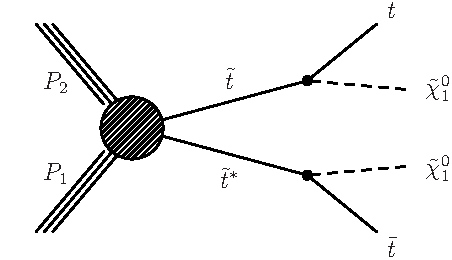
\includegraphics[width=0.5\linewidth]{plots/stopPlot/T2tt.pdf}%
        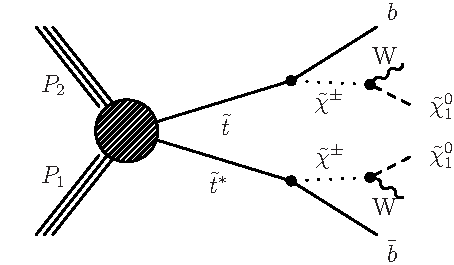
\includegraphics[width=0.5\linewidth]{plots/stopPlot/T2bw.pdf}%
	\caption{Diagram for the T2tt (left) and T2bw (right)
          simplified models.}
	\label{fig:SigDiagram}
      \end{center}
\end{figure}

The exclusion is performed using the results from the counting experiments in the signal regions
defined by \met\ and \mt\ and listed in Table~\ref{tab:srdef}. 
The cross section upper limit calculation is performed with the LandS software using the LHC-type CLs criterion. 

The signal efficiency uncertainties include the luminosity (4.4\%), lepton ID and isolation
efficiency (2\%), and trigger efficiency (3\%). The uncertainty from JES
is assessed for each scan point following the POG-recommended
procedure, by varying the jet energies by the \pt- and $\eta$-
dependent uncertainties, and propagating this to the jet multiplicity,
\met\ and \mt. The official b-tagging scale-factors for CSVM are used to compute scale
factors for the signal. The results are nearly constant across the
model parameter space, and an overall scale factor of $(98 \pm 2)\%$
is used. 
 
%However, it is instructive to get a first feeling for where the sensitivity of this search is.
%We do this in terms of ``expected limits'', assuming a null result.
%The case of an excess is quite different and more complicated.

The signal efficiency in the stop vs LSP mass plane for T2tt is shown 
for each signal region in Figures~\ref{fig:allsrlimits},
~\ref{fig:allsrlimits2} and~\ref{fig:allsrlimits3} (left). The
corresponding distributions for T2bw are shown in 
Figures~\ref{fig:allsrlimitsT2bw0p75},~\ref{fig:allsrlimits2T2bw0p75}
and~\ref{fig:allsrlimits3T2bw0p75} for x=0.75 and in Figure~\ref{fig:allsrlimitsT2bw0p5},~\ref{fig:allsrlimits2T2bw0p5} and~\ref{fig:allsrlimits3T2bw0p5}
for x=0.5 (left). The current analysis is not sensitive to the x=0.25
scenario (Figure~\ref{fig:comblimitT2bw}, bottom).

These distributions show how
challenging it is to have sensitivity near the kinematical boundaries.
The cross section upper limits, along with the
observed and expected exclusion contours, are also shown in
Figures~\ref{fig:allsrlimits},~\ref{fig:allsrlimits2}
and~\ref{fig:allsrlimits3} for T2tt, in Figures~\ref{fig:allsrlimitsT2bw0p75},~\ref{fig:allsrlimits2T2bw0p75} and~\ref{fig:allsrlimits3T2bw0p75}
for T2bw with x=0.75, and in Figure~\ref{fig:allsrlimitsT2bw0p5},~\ref{fig:allsrlimits2T2bw0p5} and~\ref{fig:allsrlimits3T2bw0p5}
for T2bw with x=0.5 (right).
The complementarity of the different signal regions is readily apparent.  
The sensitivity to low (high) stop masses comes from the 
low (high) \met\ signal regions.

\begin{figure}[hbt]
  \begin{center}
        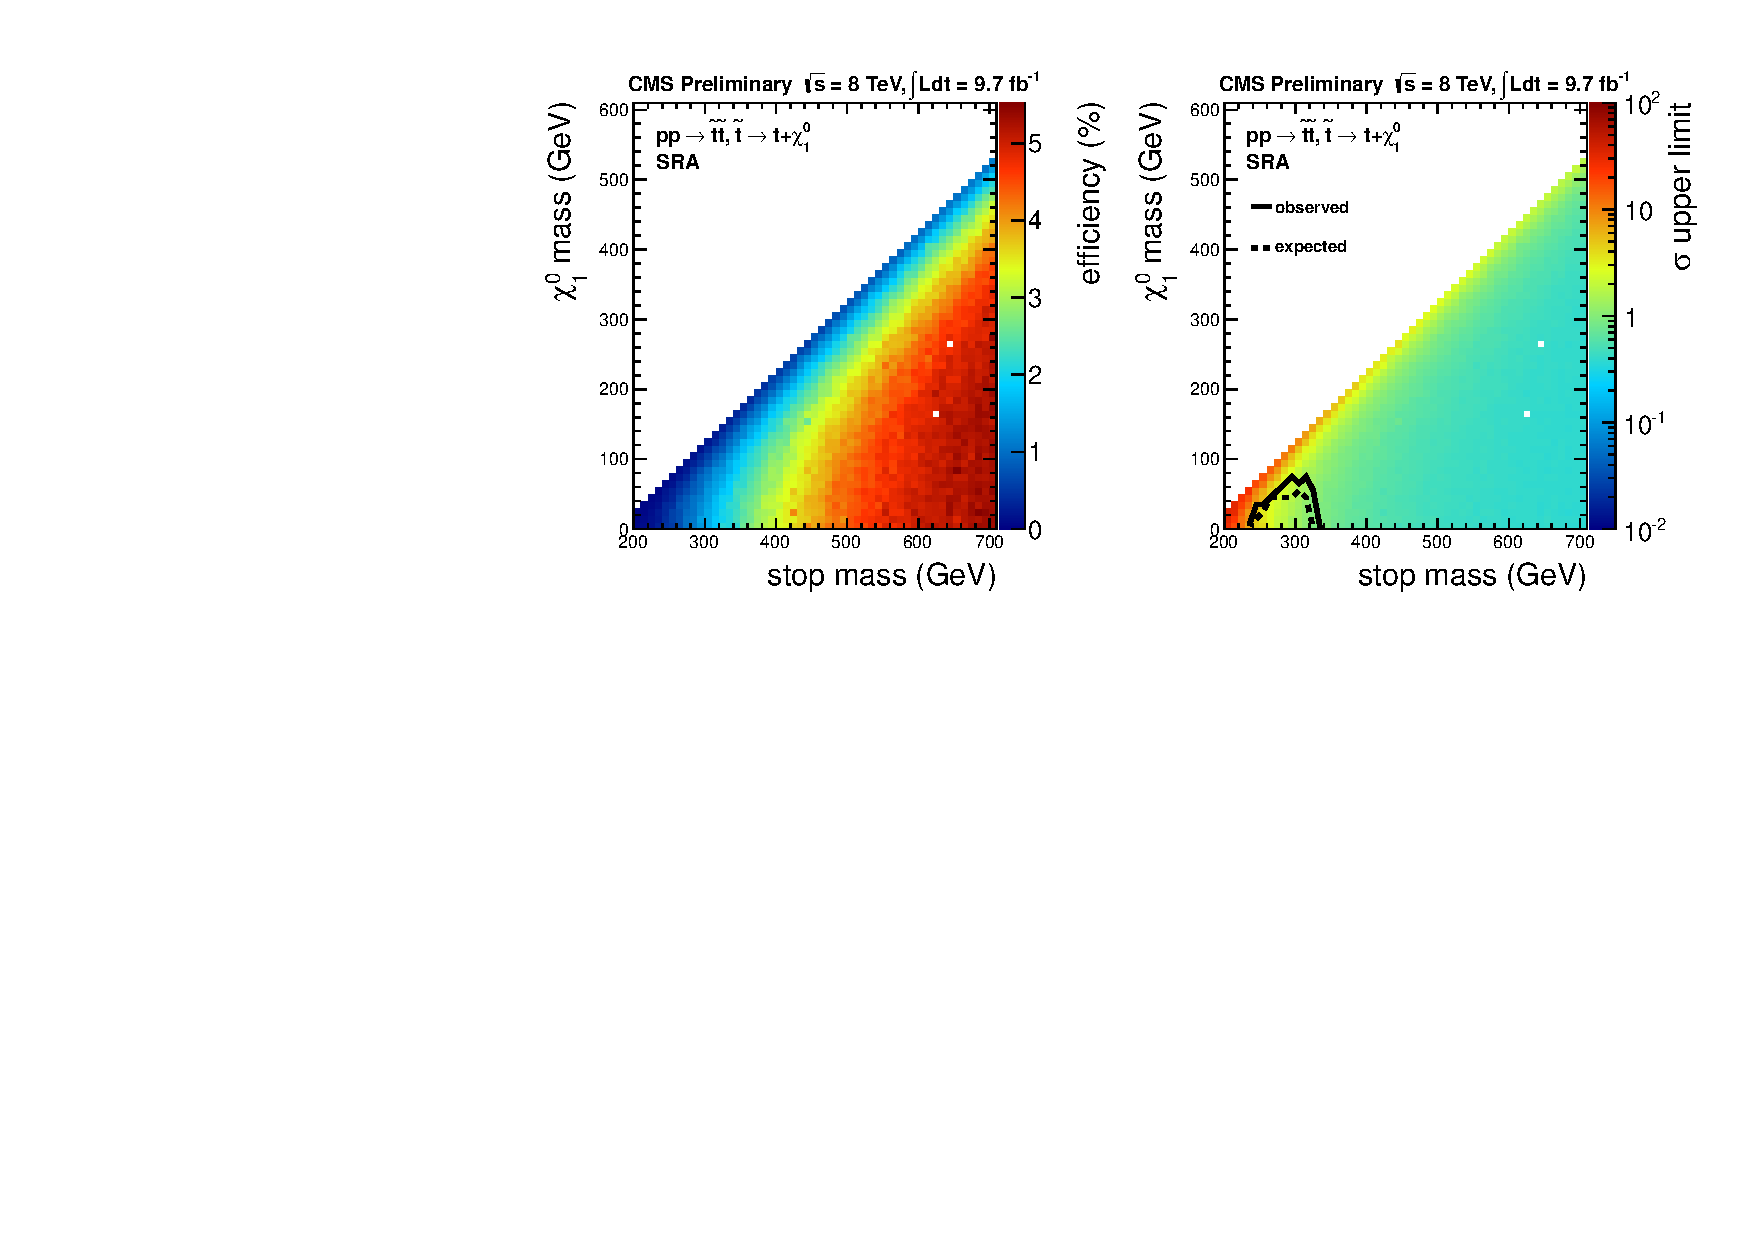
\includegraphics[width=1.\linewidth]{plots/T2tt_SRA.pdf}
        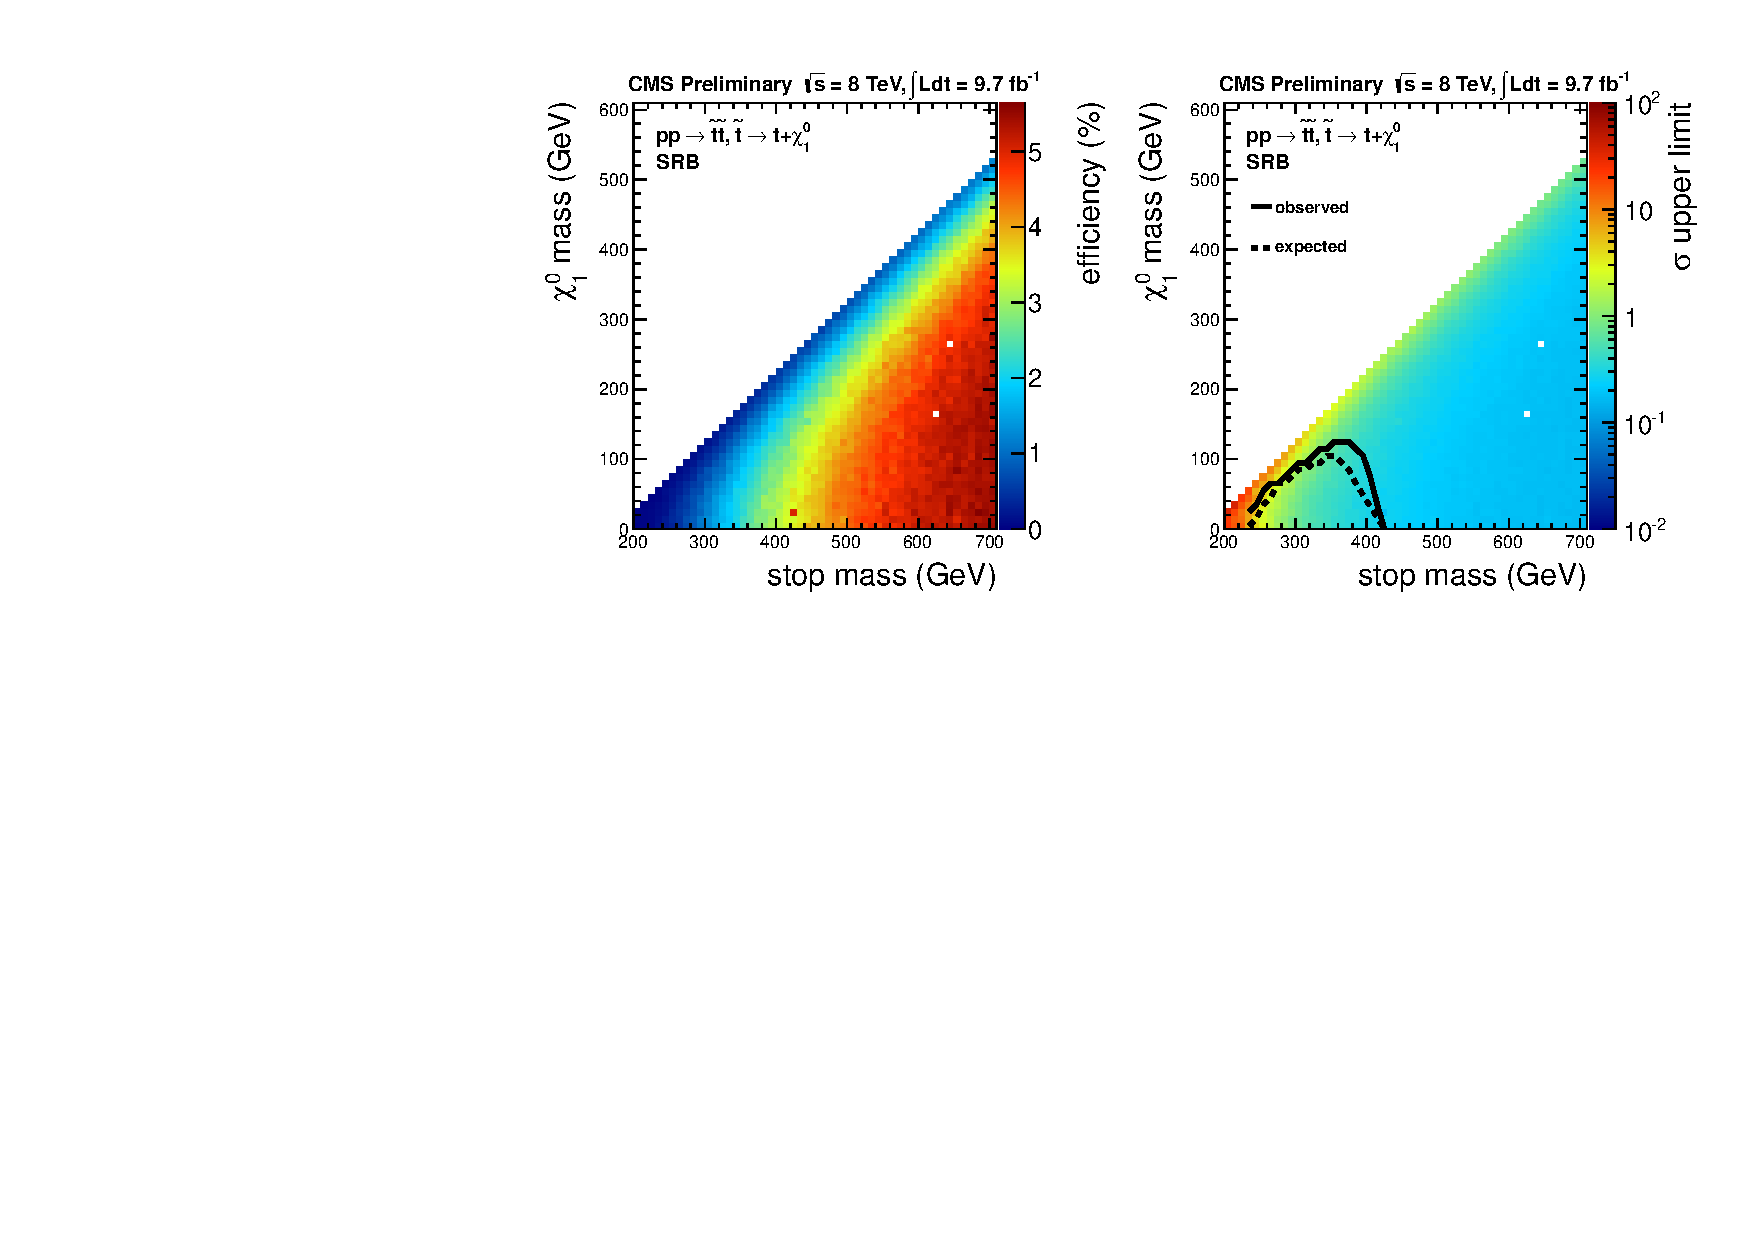
\includegraphics[width=1.\linewidth]{plots/T2tt_SRB.pdf}
        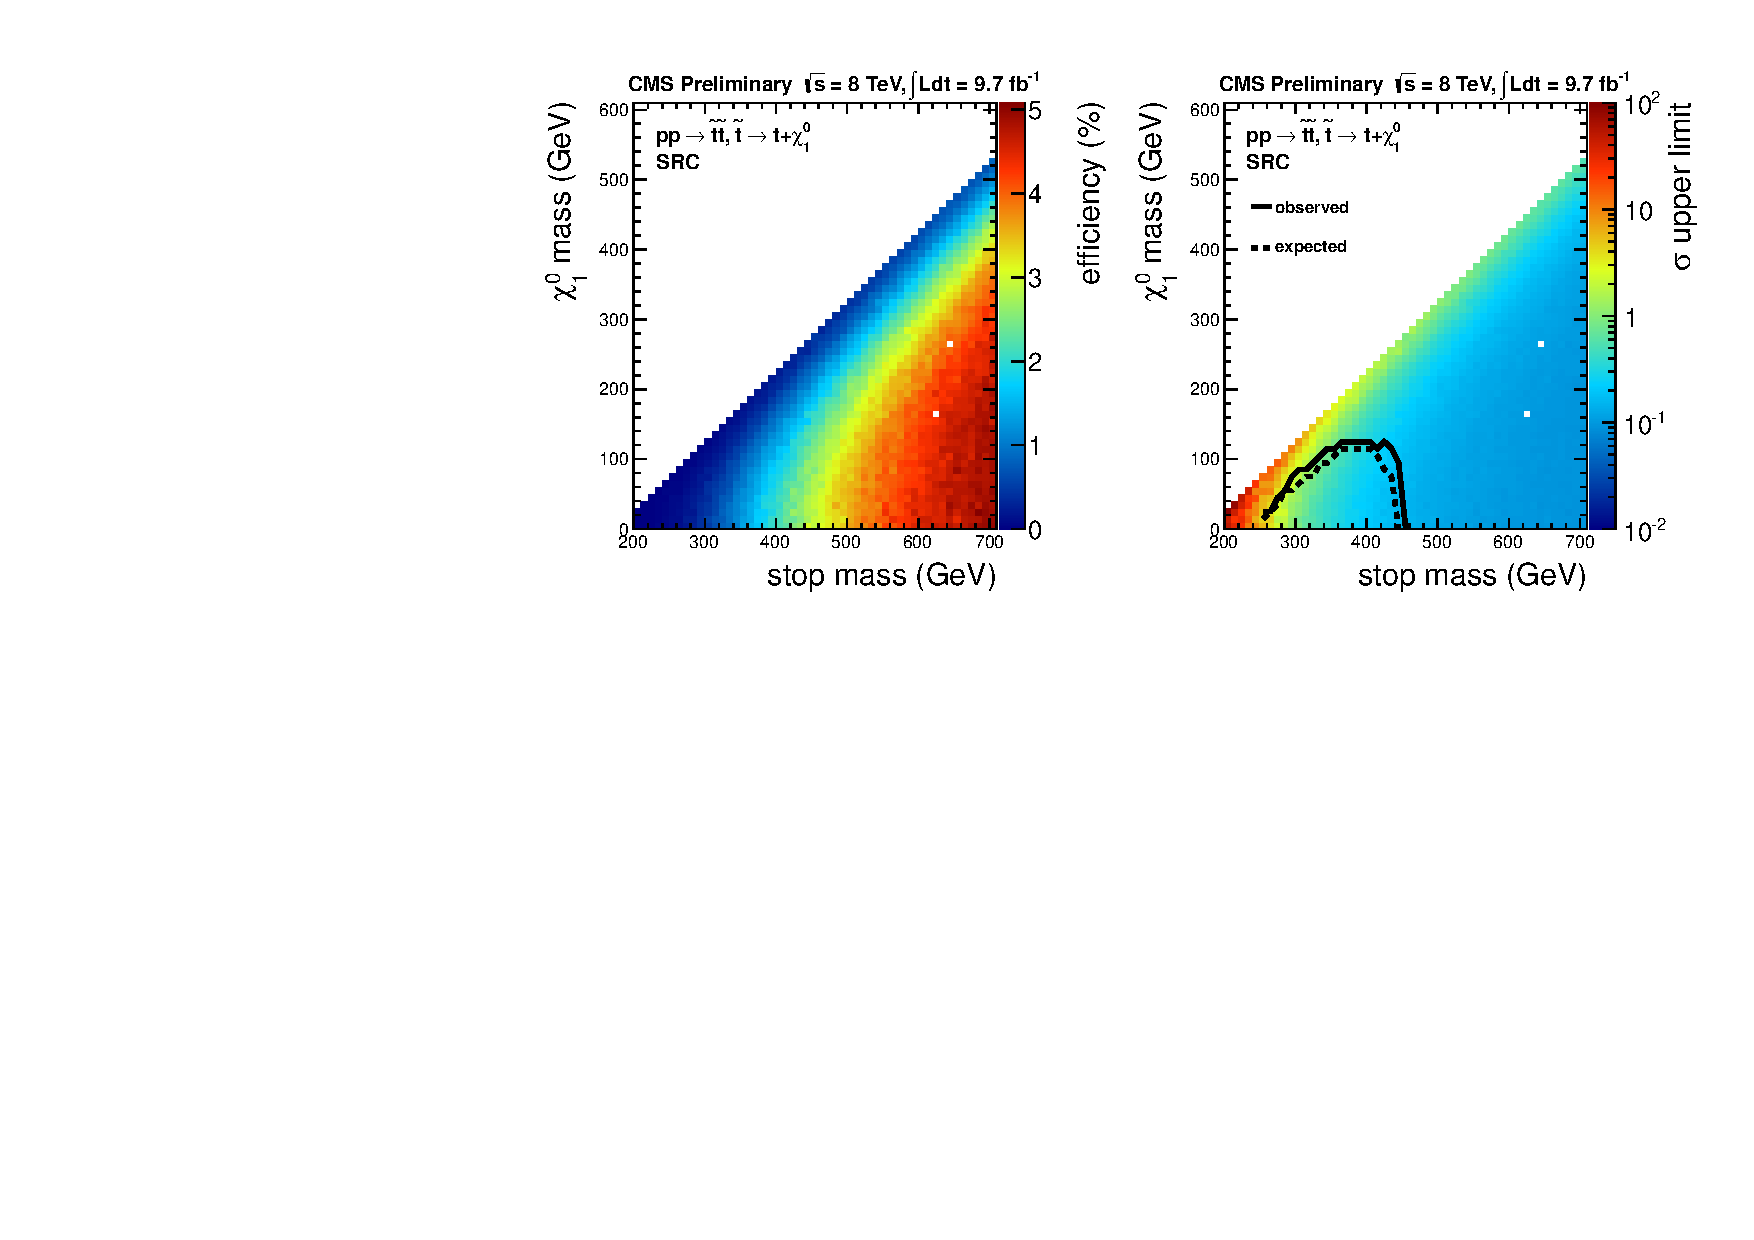
\includegraphics[width=1.\linewidth]{plots/T2tt_SRC.pdf}
    \caption{Signal efficiency (left) and cross section upper limit
      (right) for the T2tt model, showing both the expected and
      observed exclusion contours. The results for signal regions SRA (top),
      SRB (middle) and SRC (bottom) are shown separately.}
\label{fig:allsrlimits}
      \end{center}
\end{figure}

\begin{figure}[hbt]
  \begin{center}
        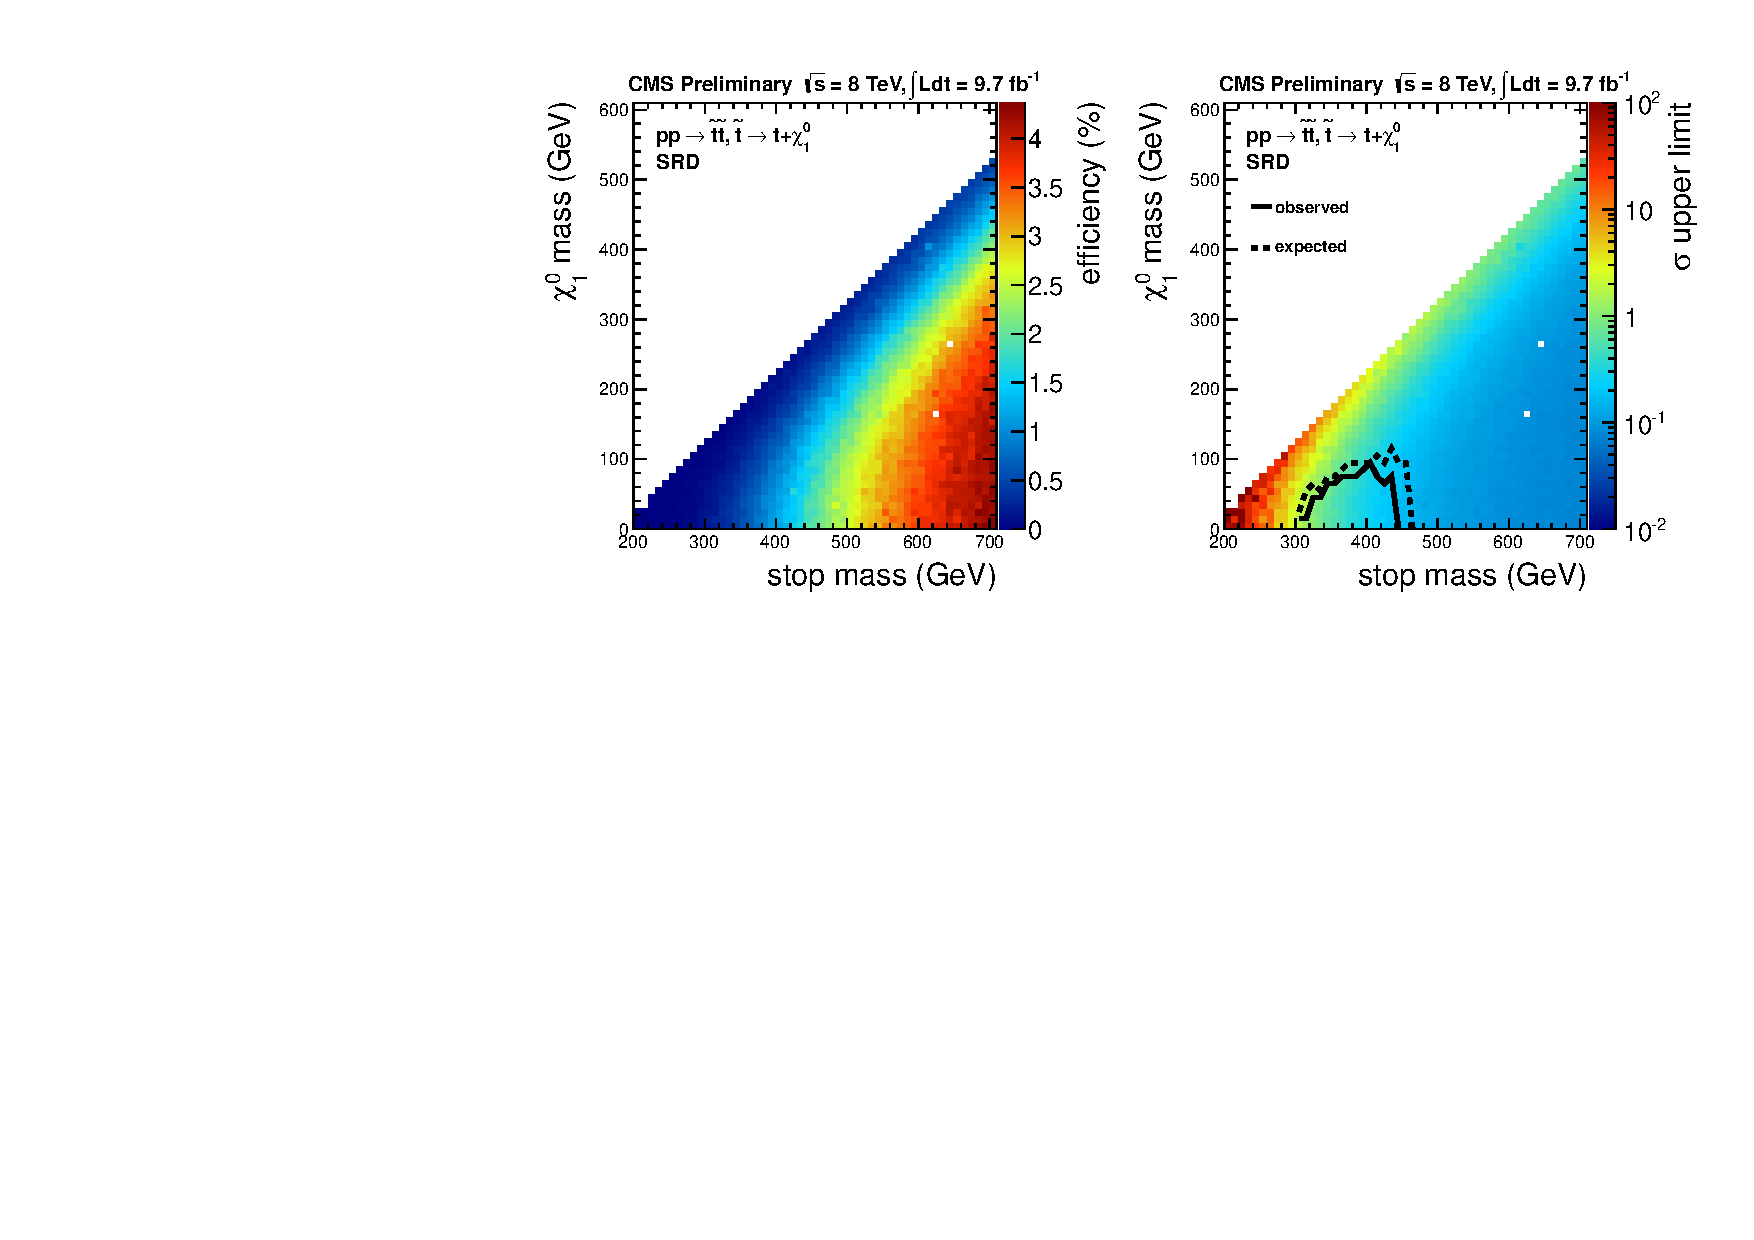
\includegraphics[width=1.\linewidth]{plots/T2tt_SRD.pdf}
        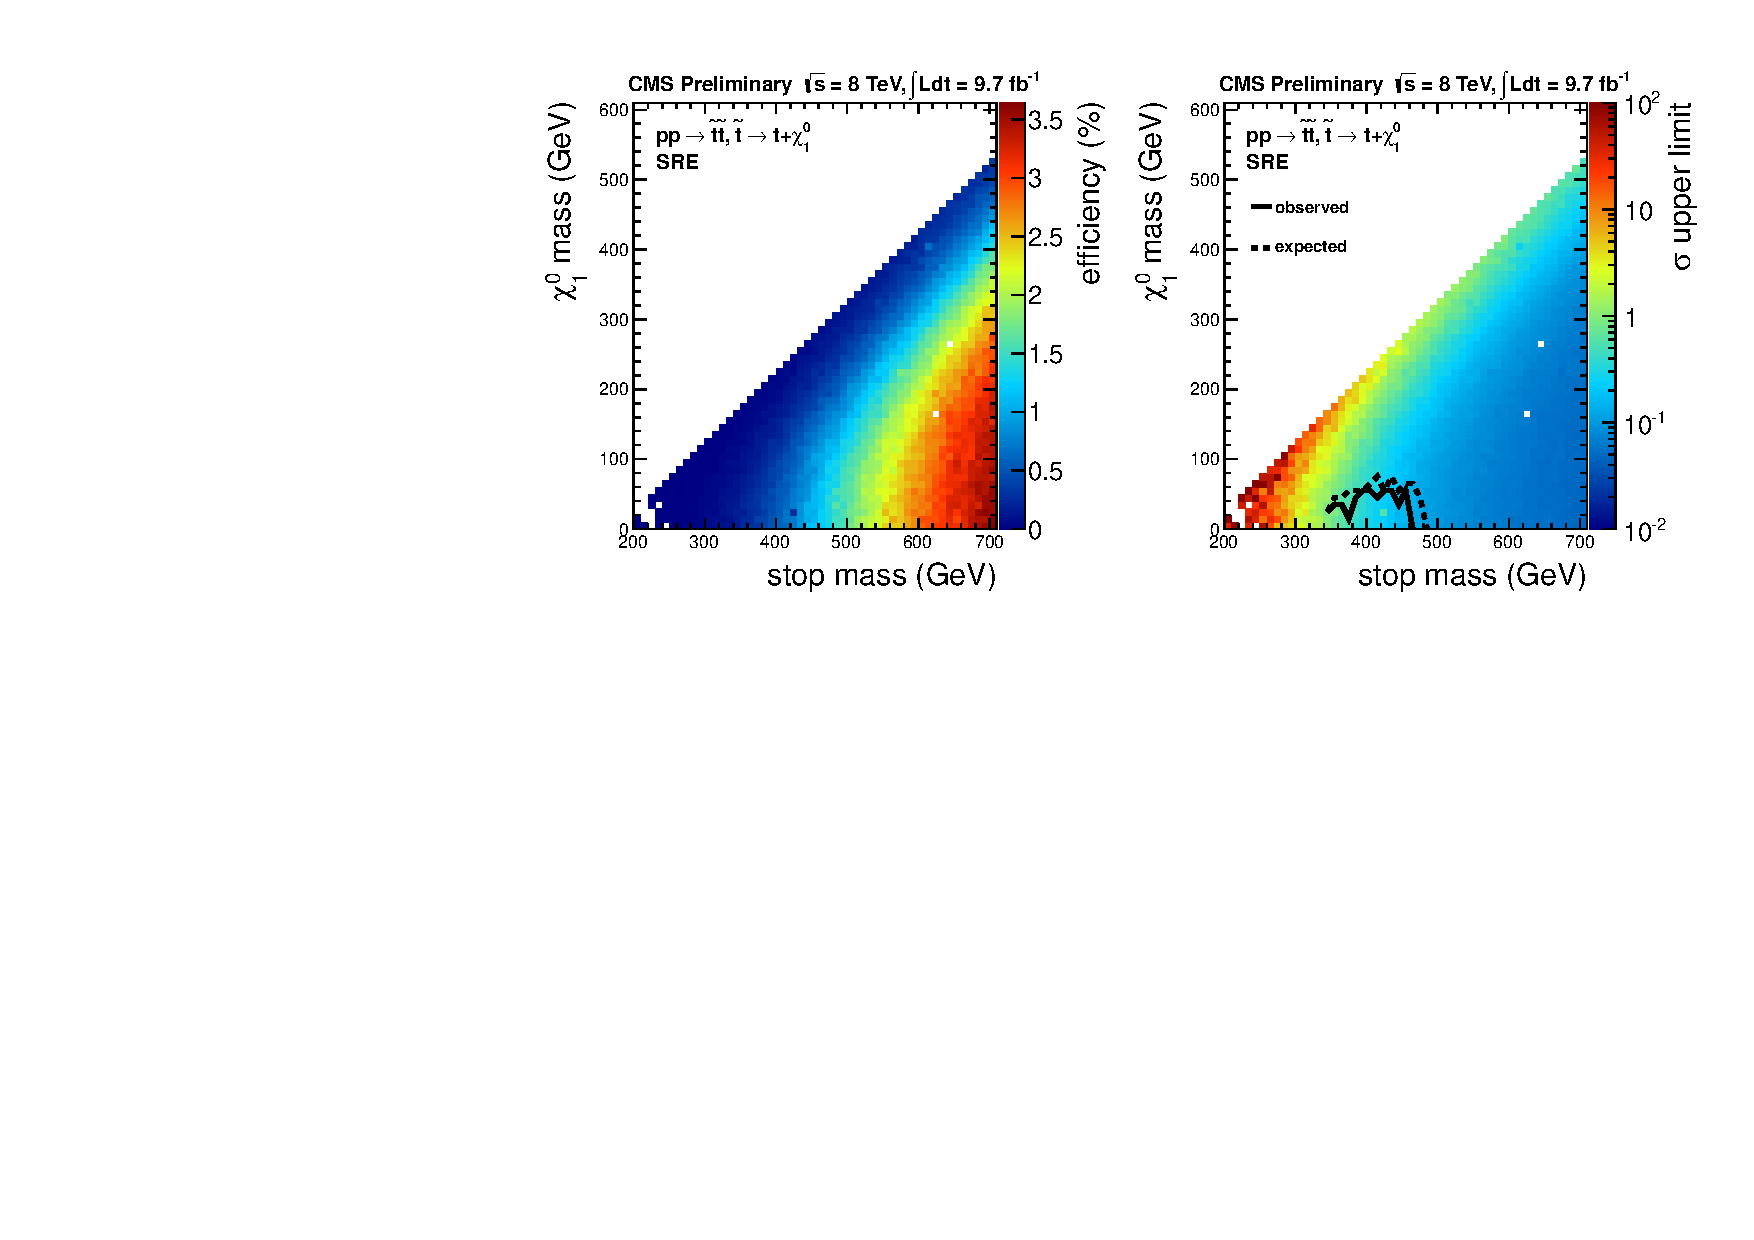
\includegraphics[width=1.\linewidth]{plots/T2tt_SRE.pdf}
    \caption{Signal efficiency (left) and cross section upper limit
      (right) for the T2tt model, showing both the expected and
      observed exclusion contours. The results for signal regions SRD (top),
      and SRE (bottom) are shown separately.}
\label{fig:allsrlimits2}
      \end{center}
\end{figure}

\begin{figure}[hbt]
  \begin{center}
        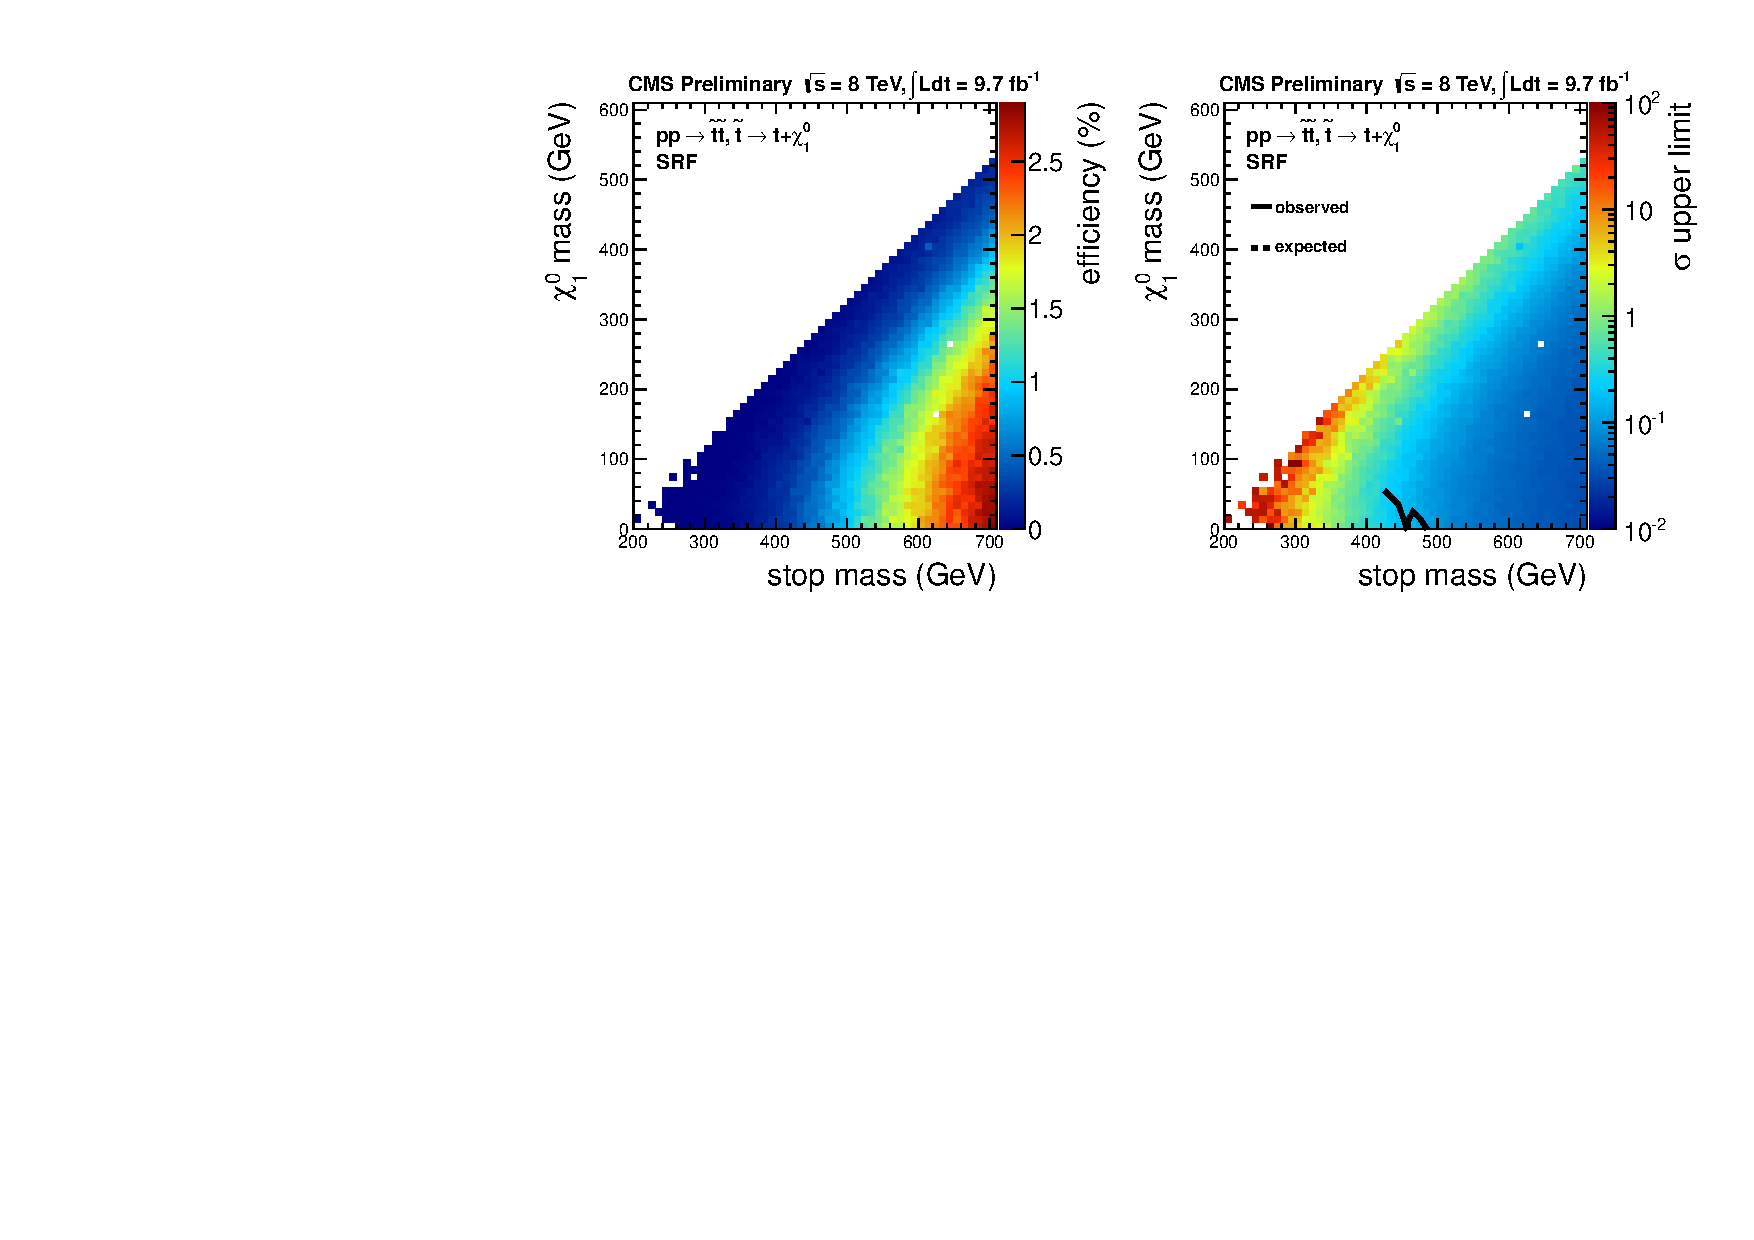
\includegraphics[width=1.\linewidth]{plots/T2tt_SRF.pdf}
        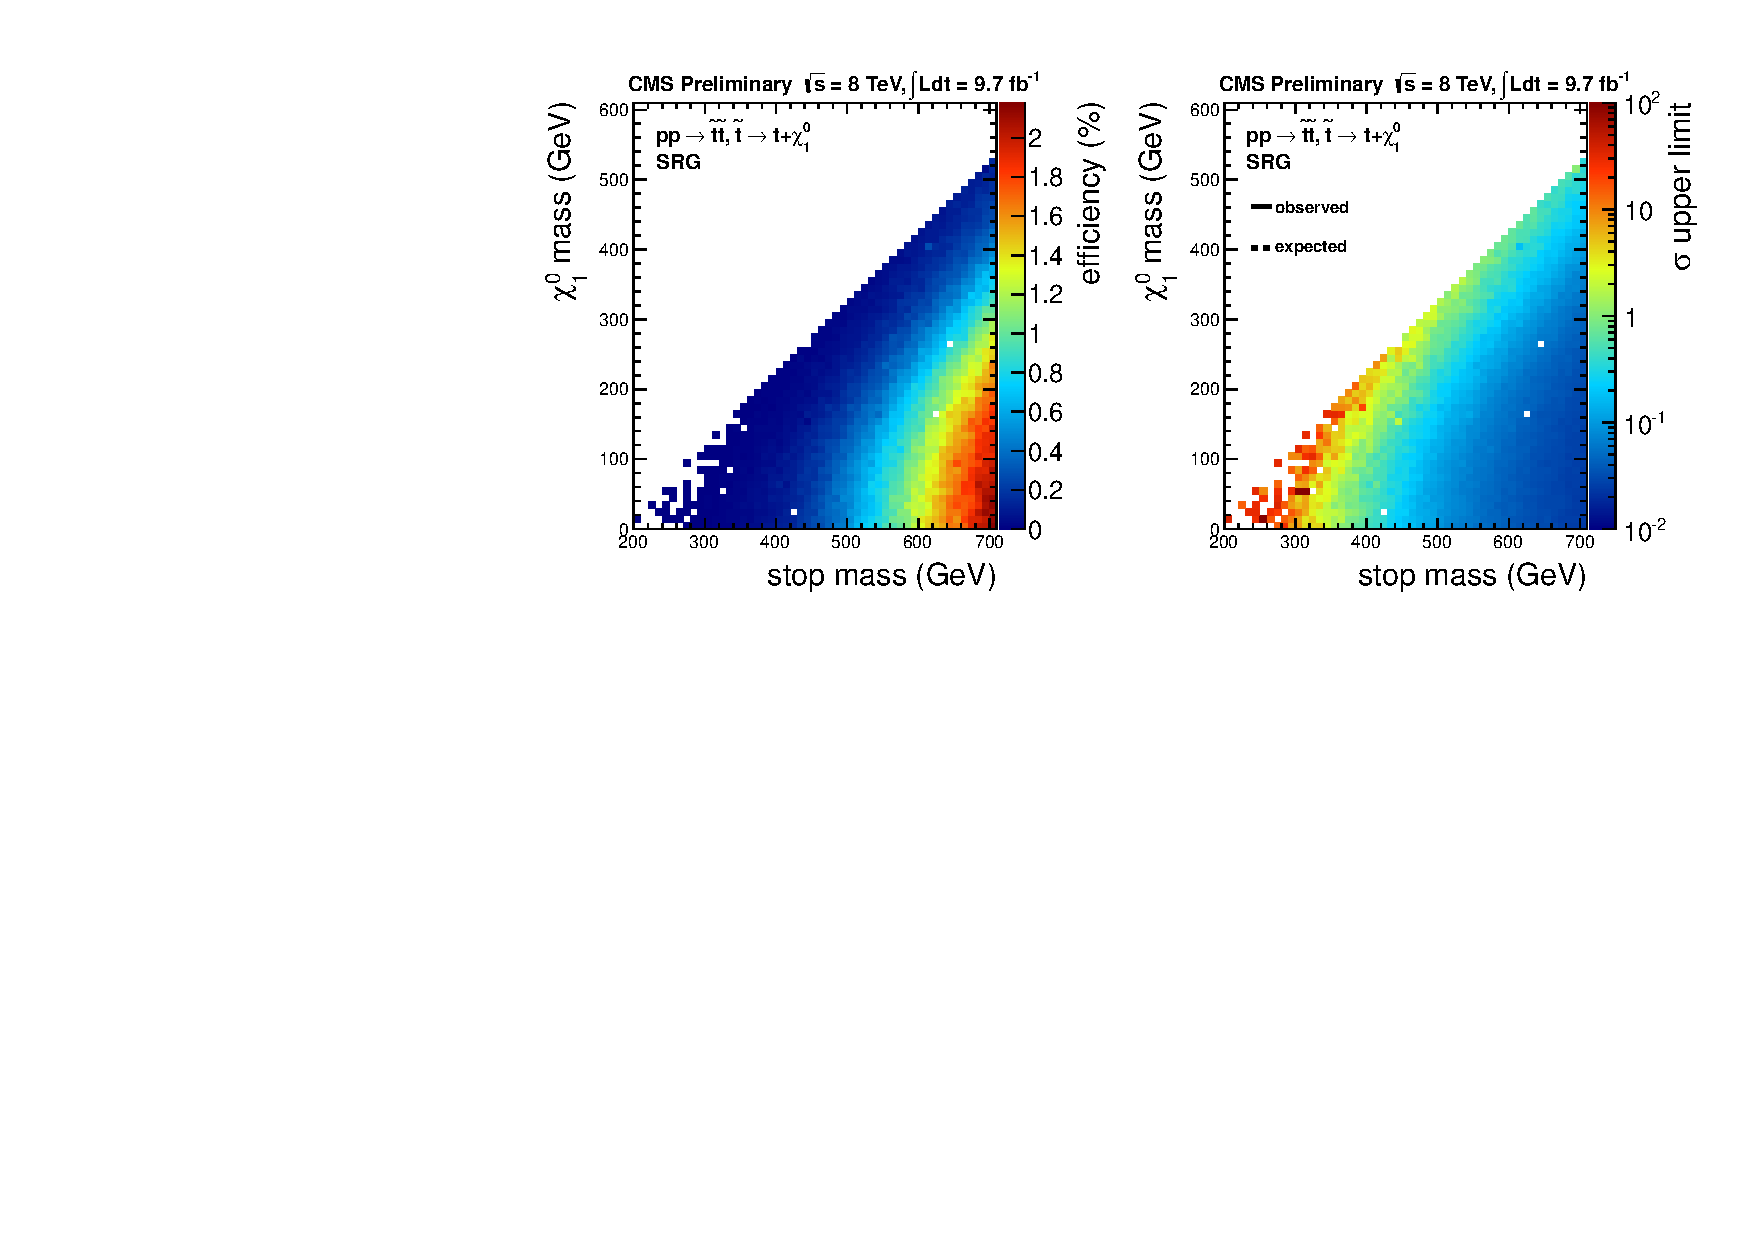
\includegraphics[width=1.\linewidth]{plots/T2tt_SRG.pdf}
    \caption{Signal efficiency (left) and cross section upper limit
      (right) for the T2tt model, showing both the expected and
      observed exclusion contours. The results for signal regions SRF (top),
      and SRG (bottom) are shown separately.}
\label{fig:allsrlimits3}
      \end{center}
\end{figure}

\begin{figure}[hbt]
  \begin{center}
        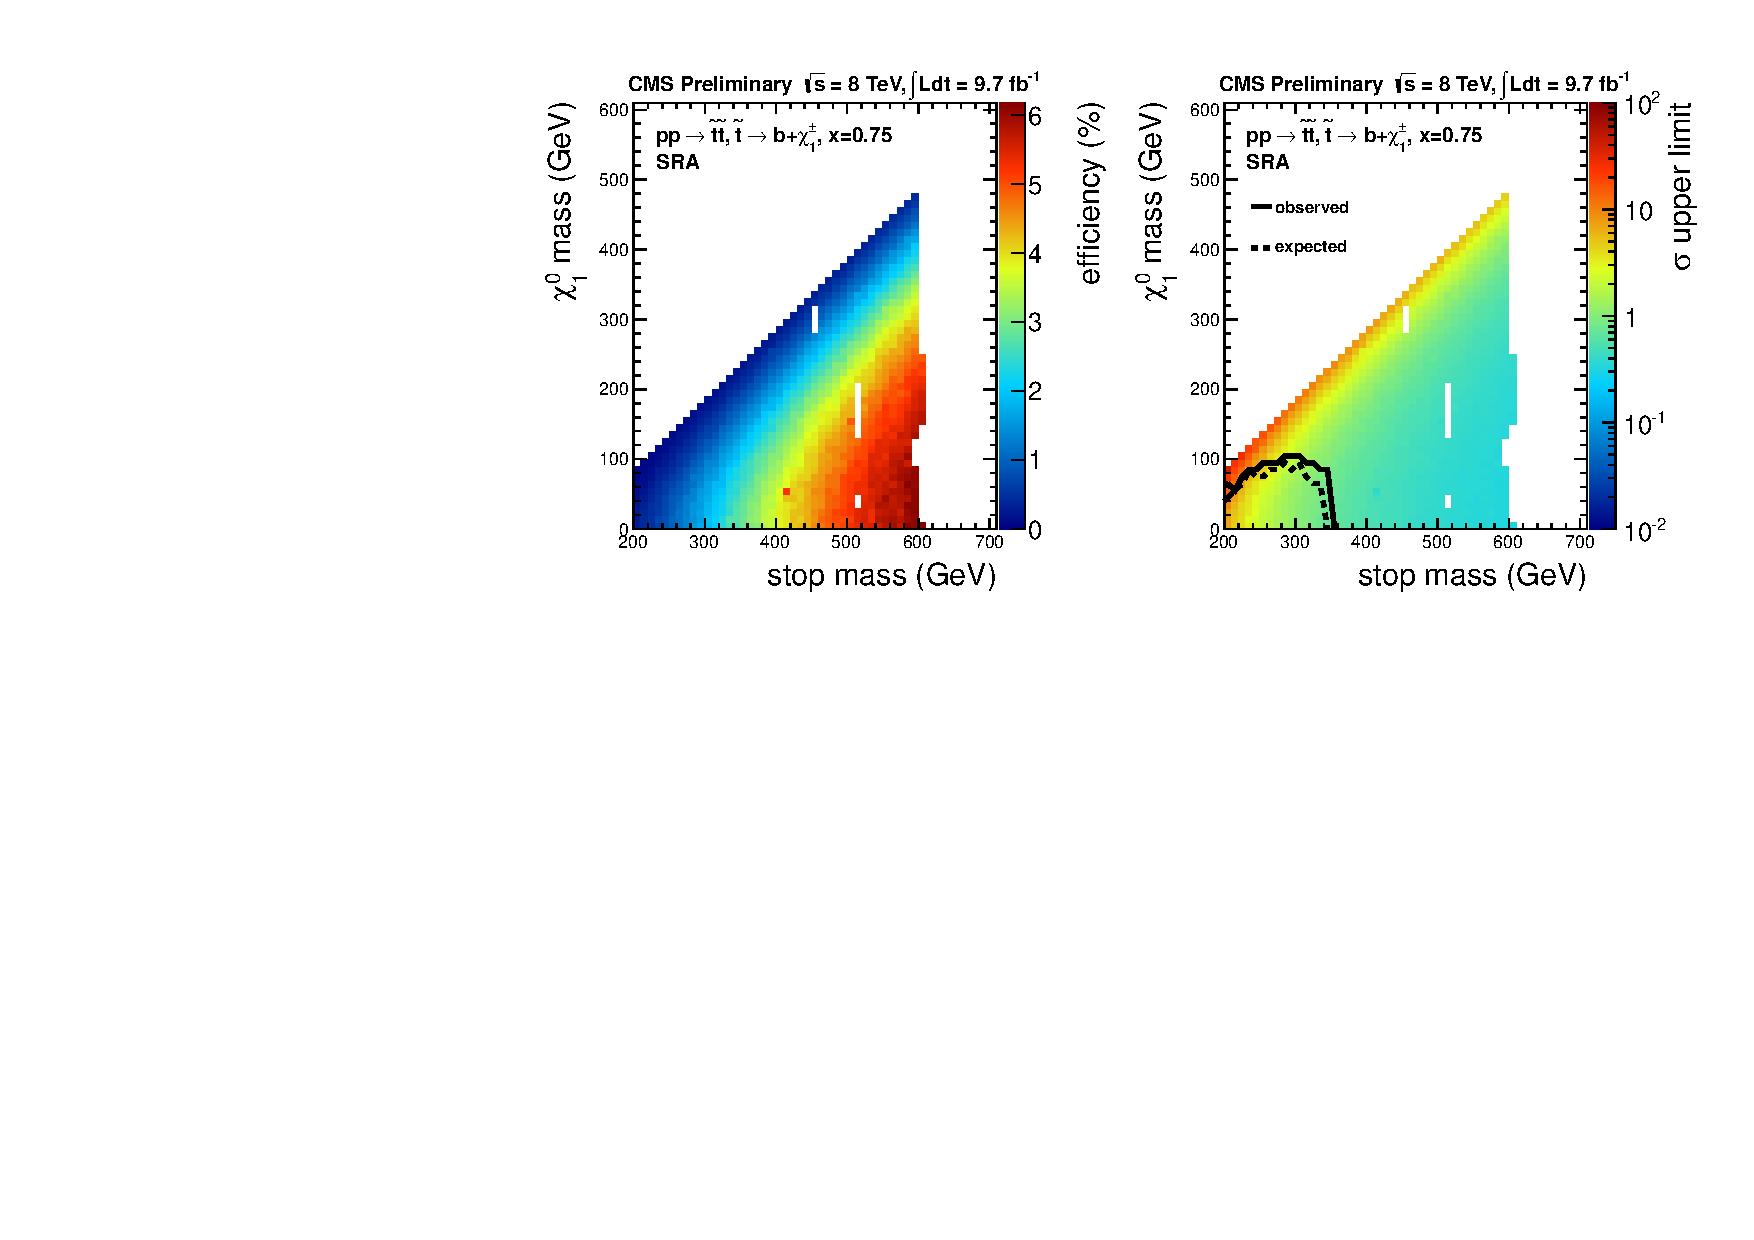
\includegraphics[width=1.\linewidth]{plots/T2bw_x75_SRA.pdf}
        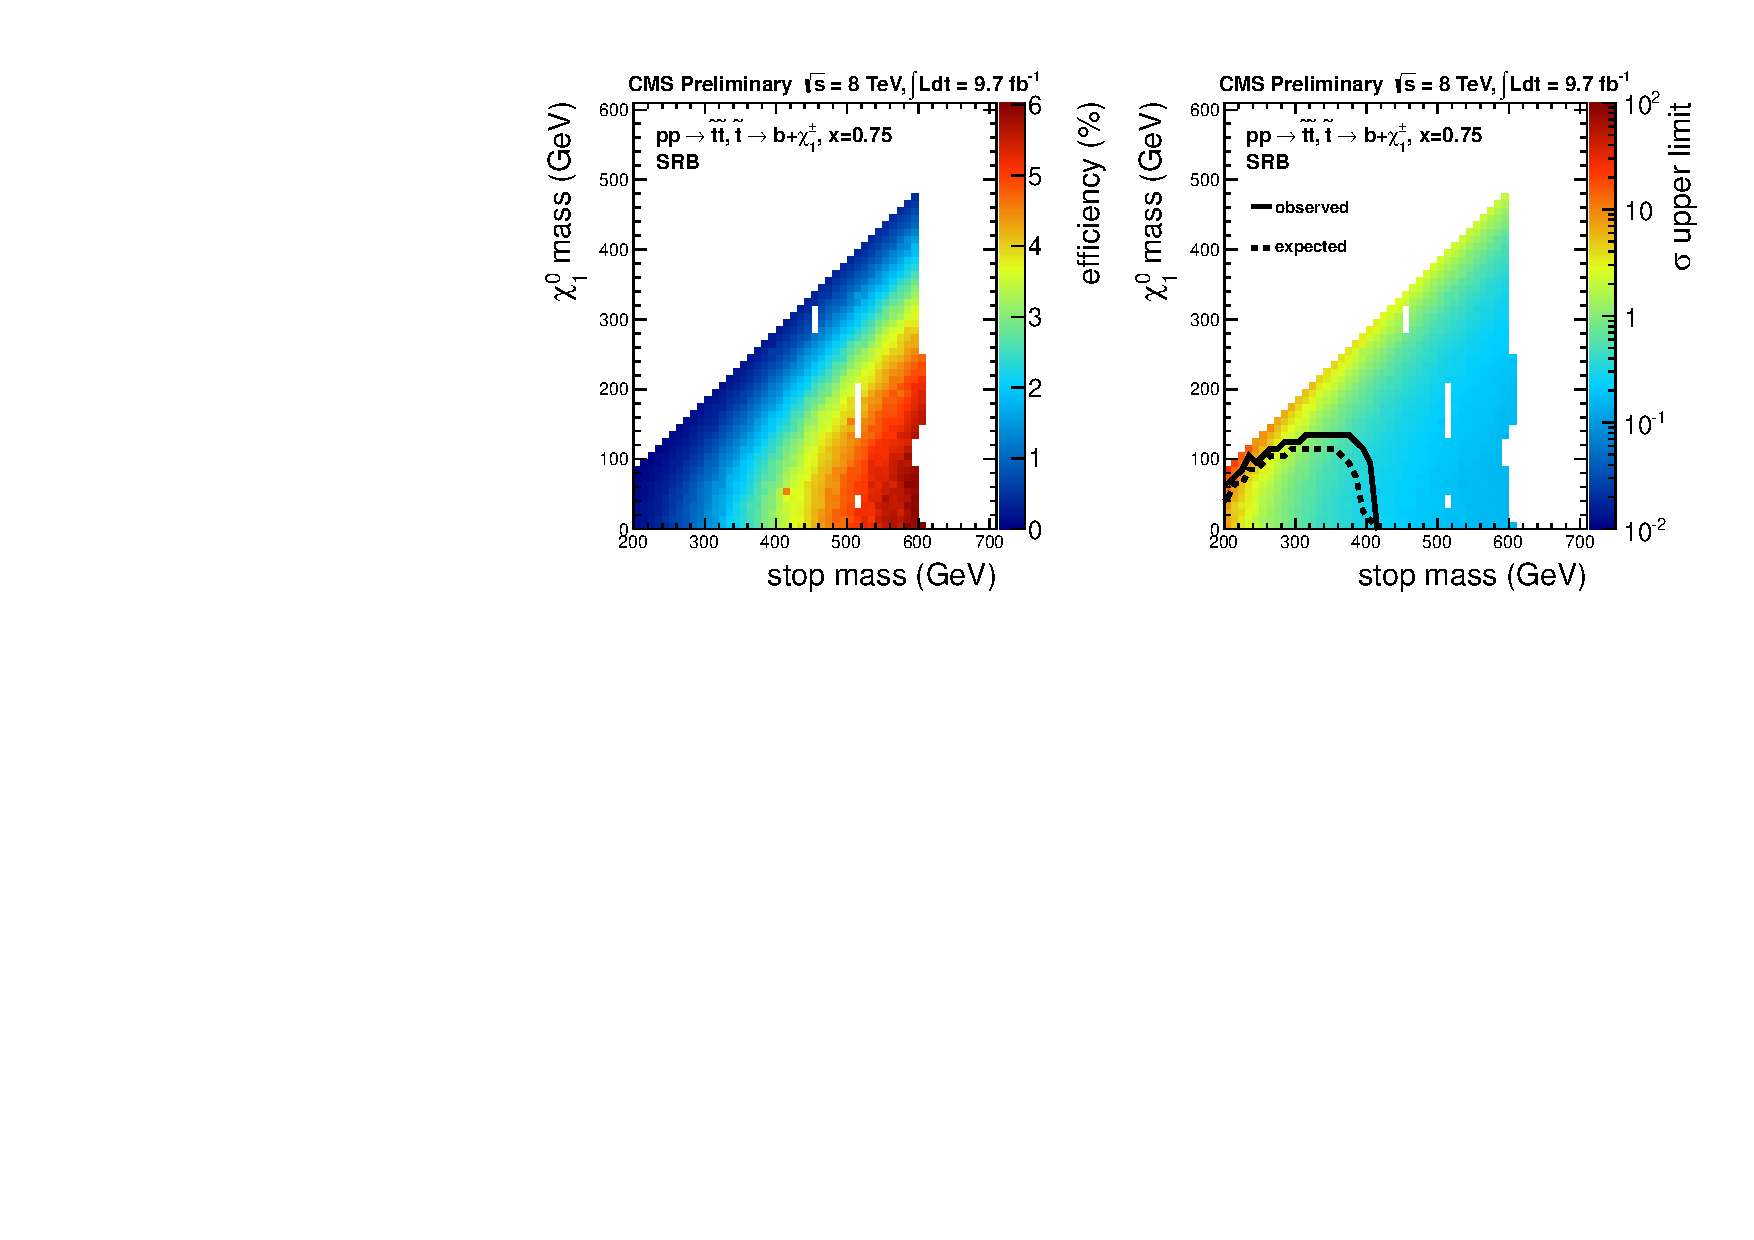
\includegraphics[width=1.\linewidth]{plots/T2bw_x75_SRB.pdf}
        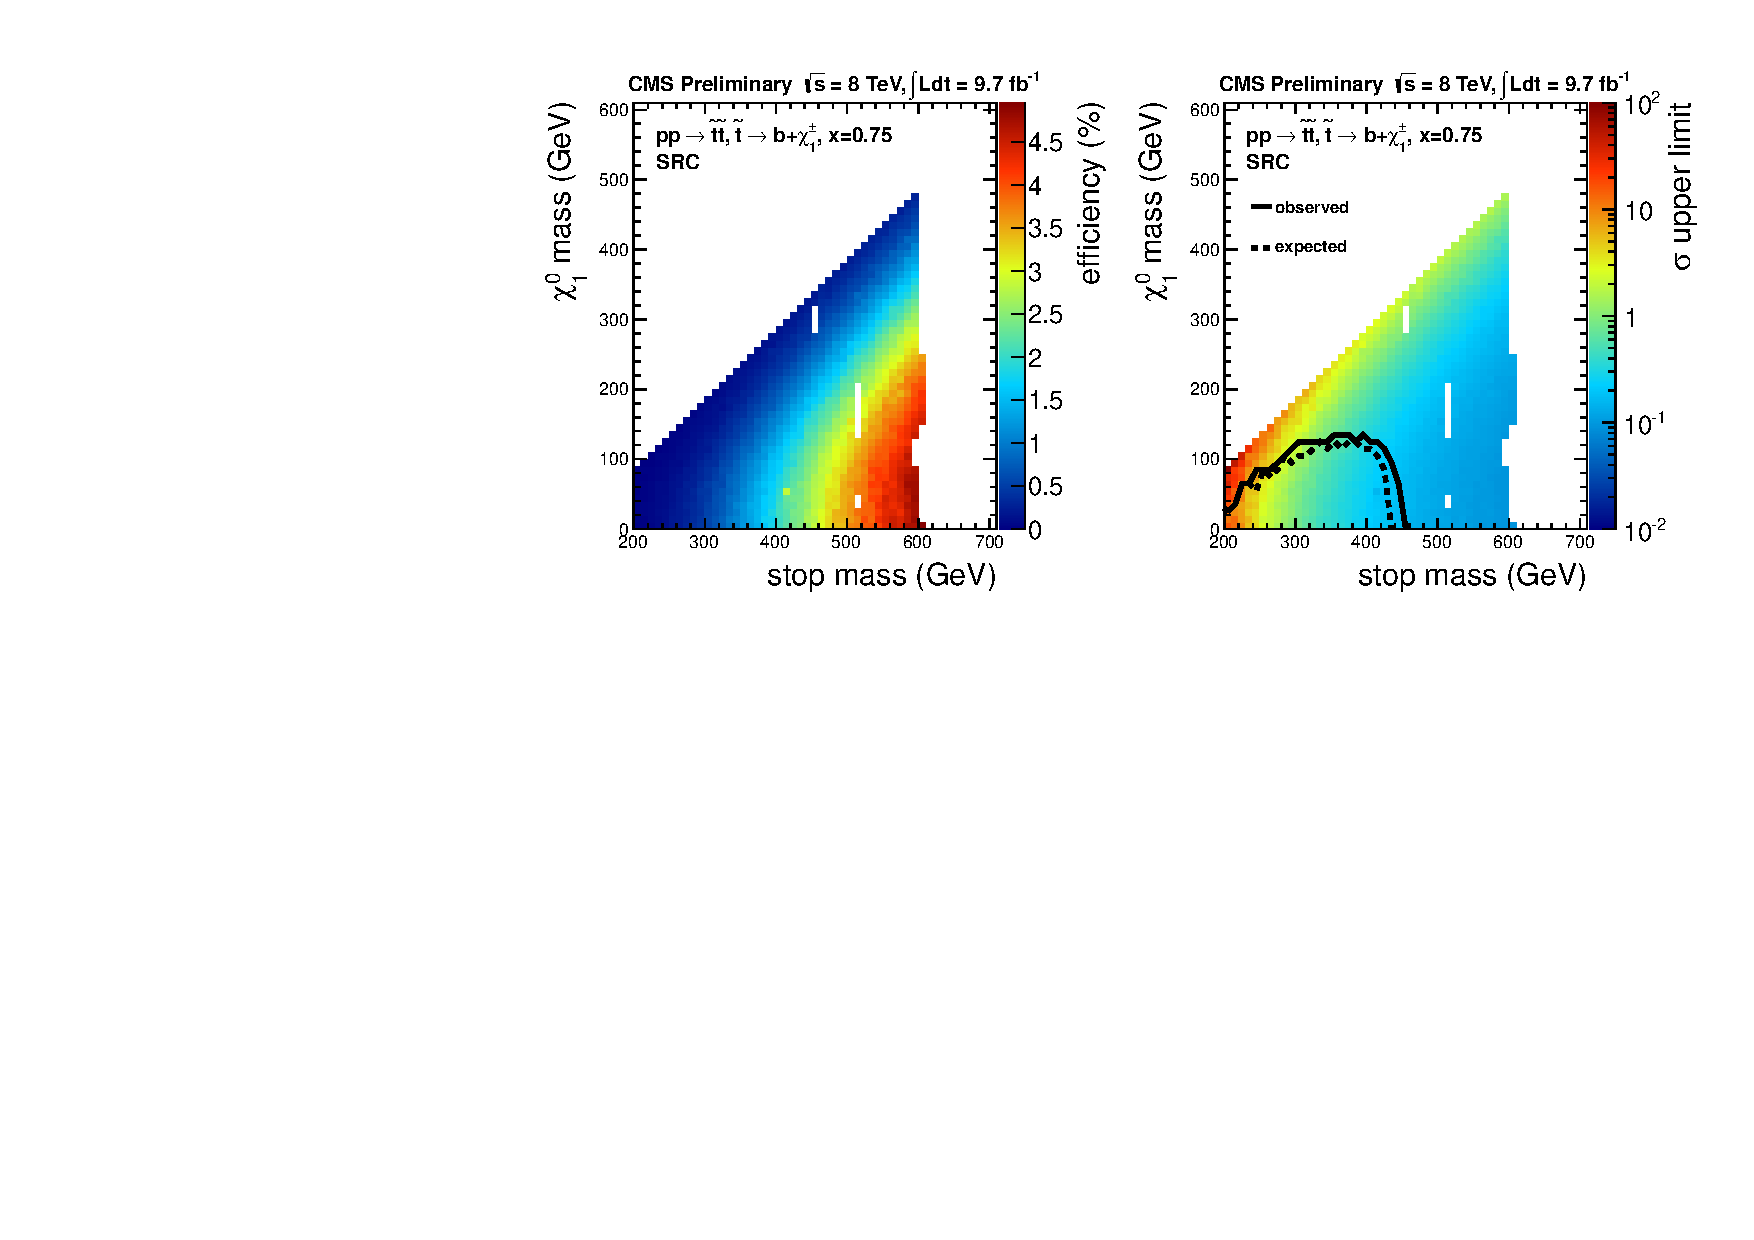
\includegraphics[width=1.\linewidth]{plots/T2bw_x75_SRC.pdf}
    \caption{Signal efficiency (left) and cross section upper limit
      (right) for the T2bw model with x=0.75, showing both the expected and
      observed exclusion contours. The results for signal regions SRA (top),
      SRB (middle) and SRC (bottom) are shown separately.}
\label{fig:allsrlimitsT2bw0p75}
      \end{center}
\end{figure}

\begin{figure}[hbt]
  \begin{center}
        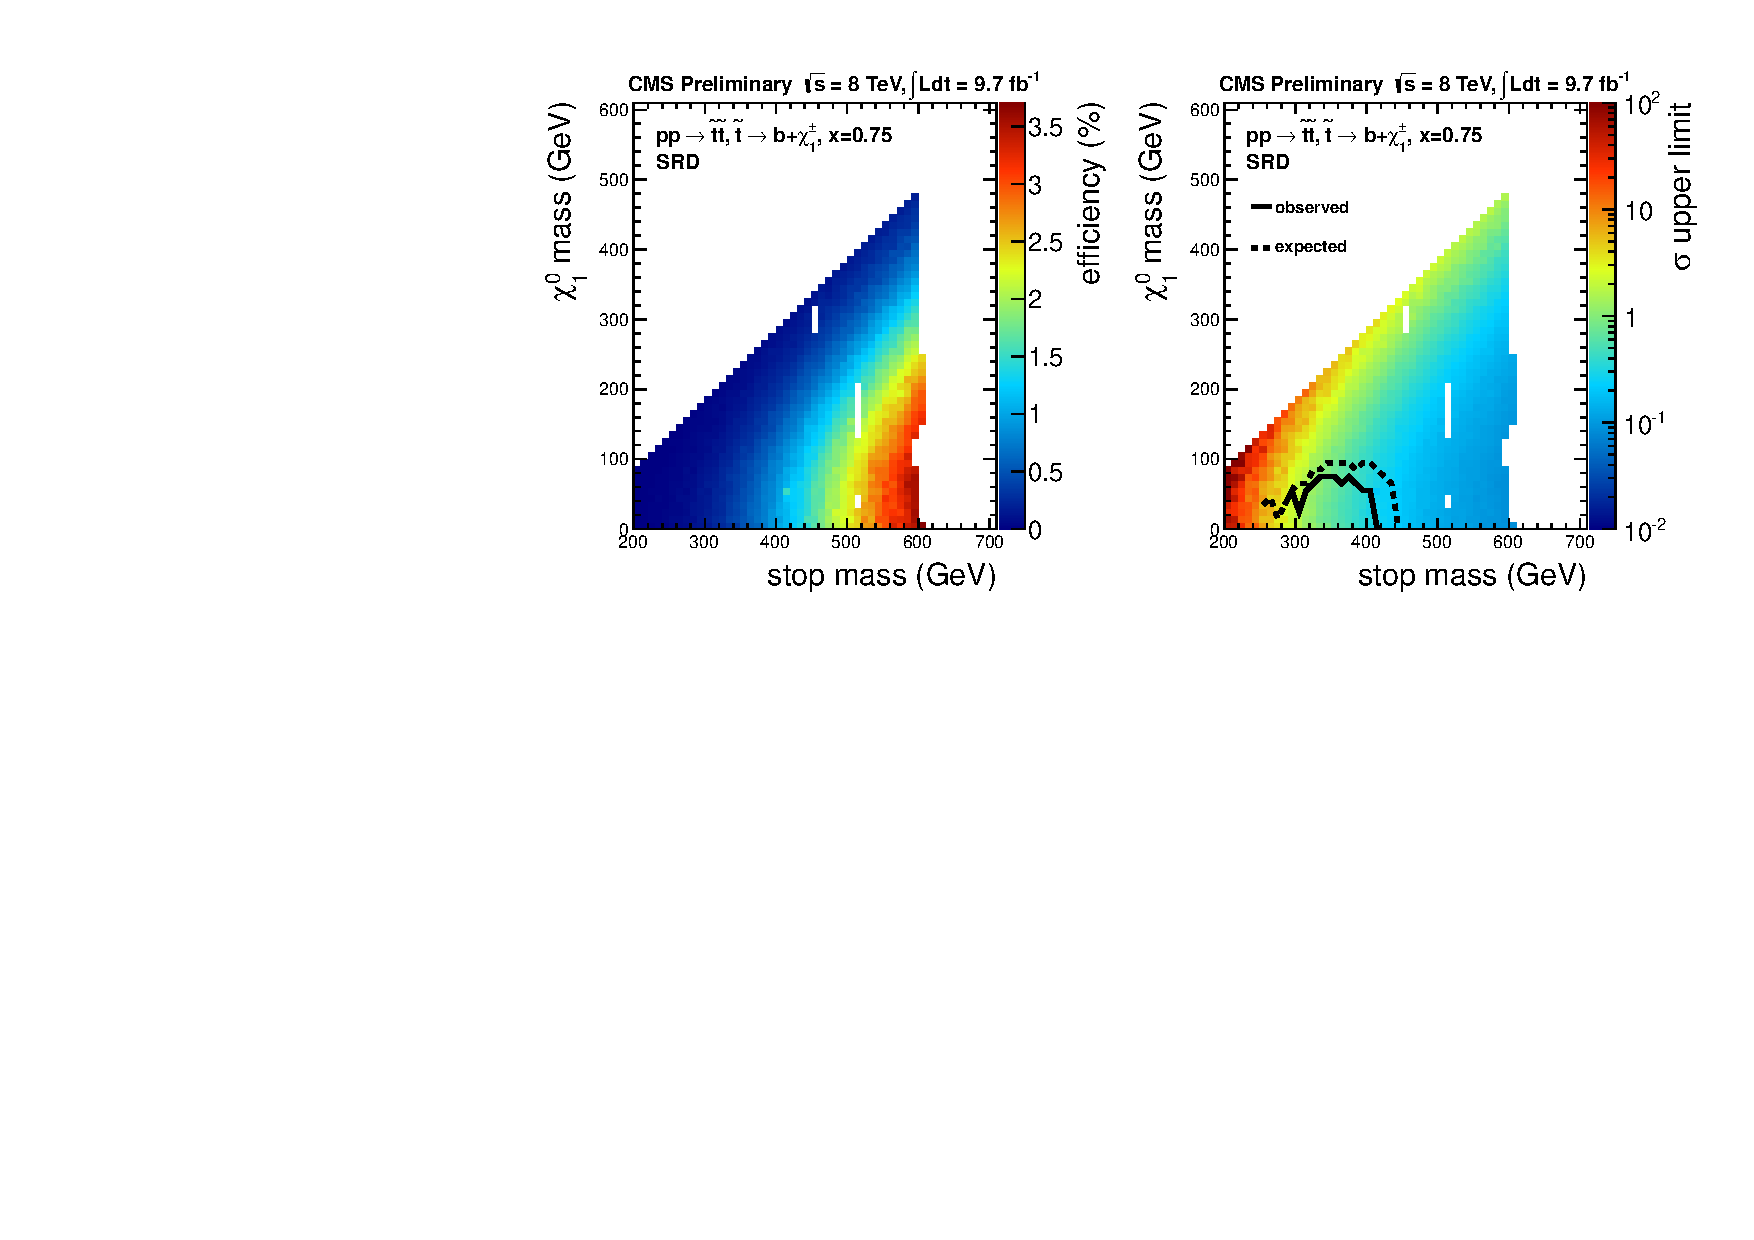
\includegraphics[width=1.\linewidth]{plots/T2bw_x75_SRD.pdf}
        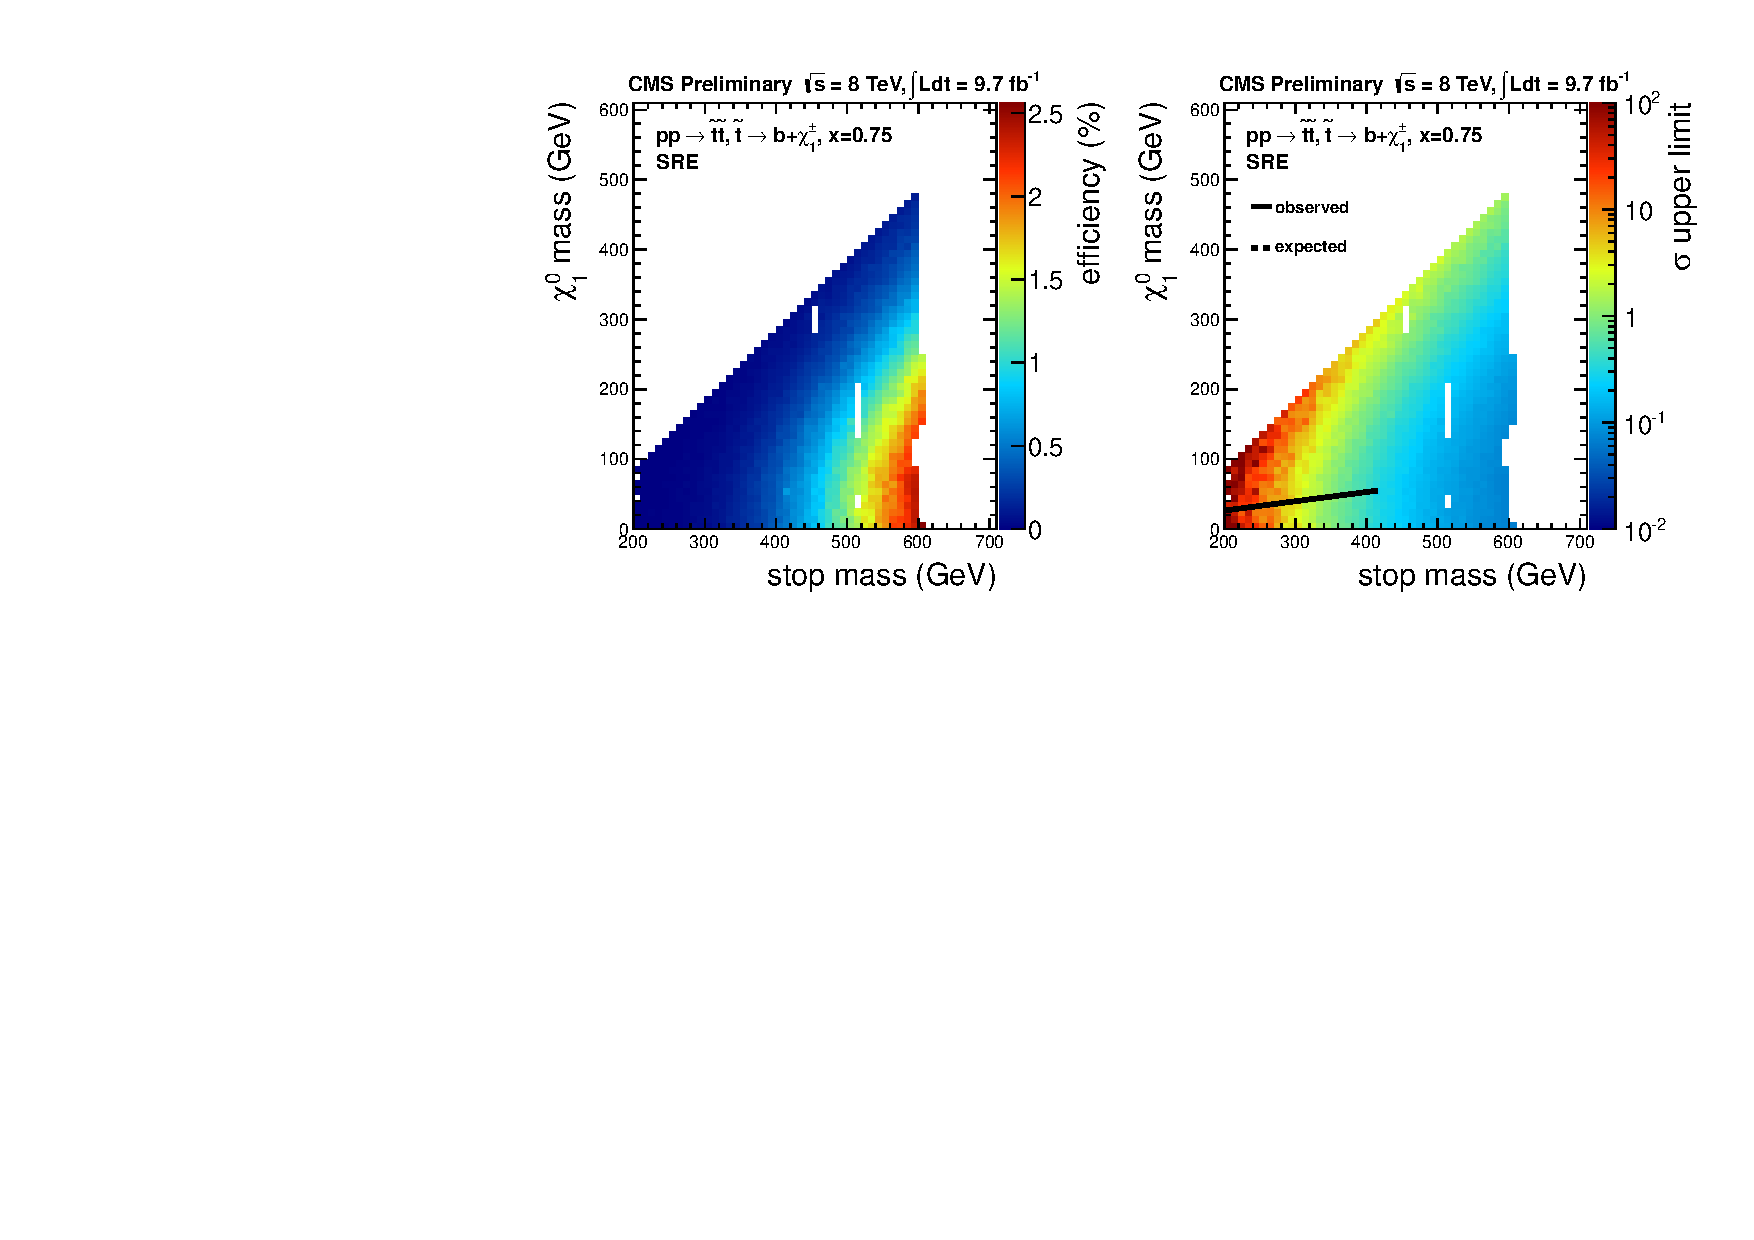
\includegraphics[width=1.\linewidth]{plots/T2bw_x75_SRE.pdf}
    \caption{Signal efficiency (left) and cross section upper limit
      (right) for the T2bw model with x=0.75, showing both the expected and
      observed exclusion contours. The results for signal regions SRD (top),
      and SRE (bottom) are shown separately.}
\label{fig:allsrlimits2T2bw0p75}
      \end{center}
\end{figure}

\begin{figure}[hbt]
  \begin{center}
        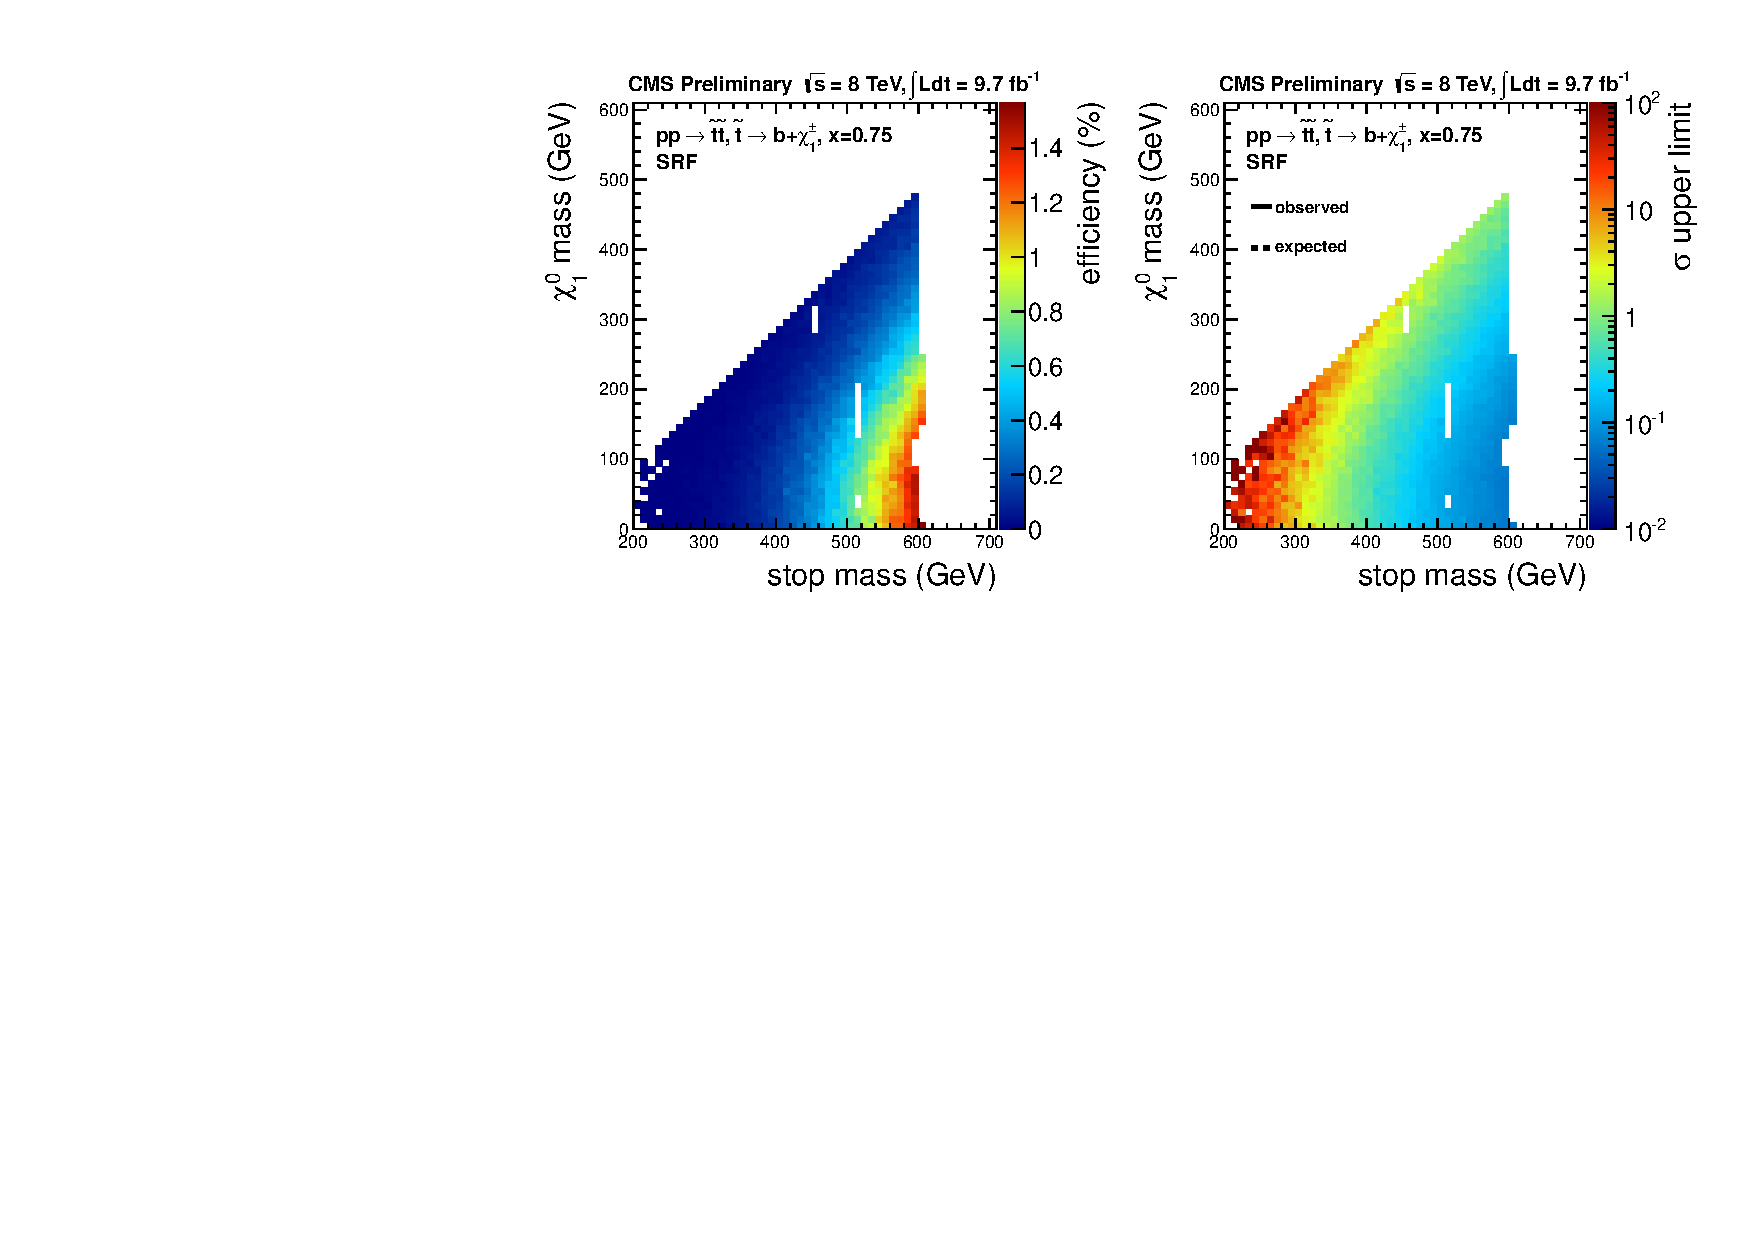
\includegraphics[width=1.\linewidth]{plots/T2bw_x75_SRF.pdf}
        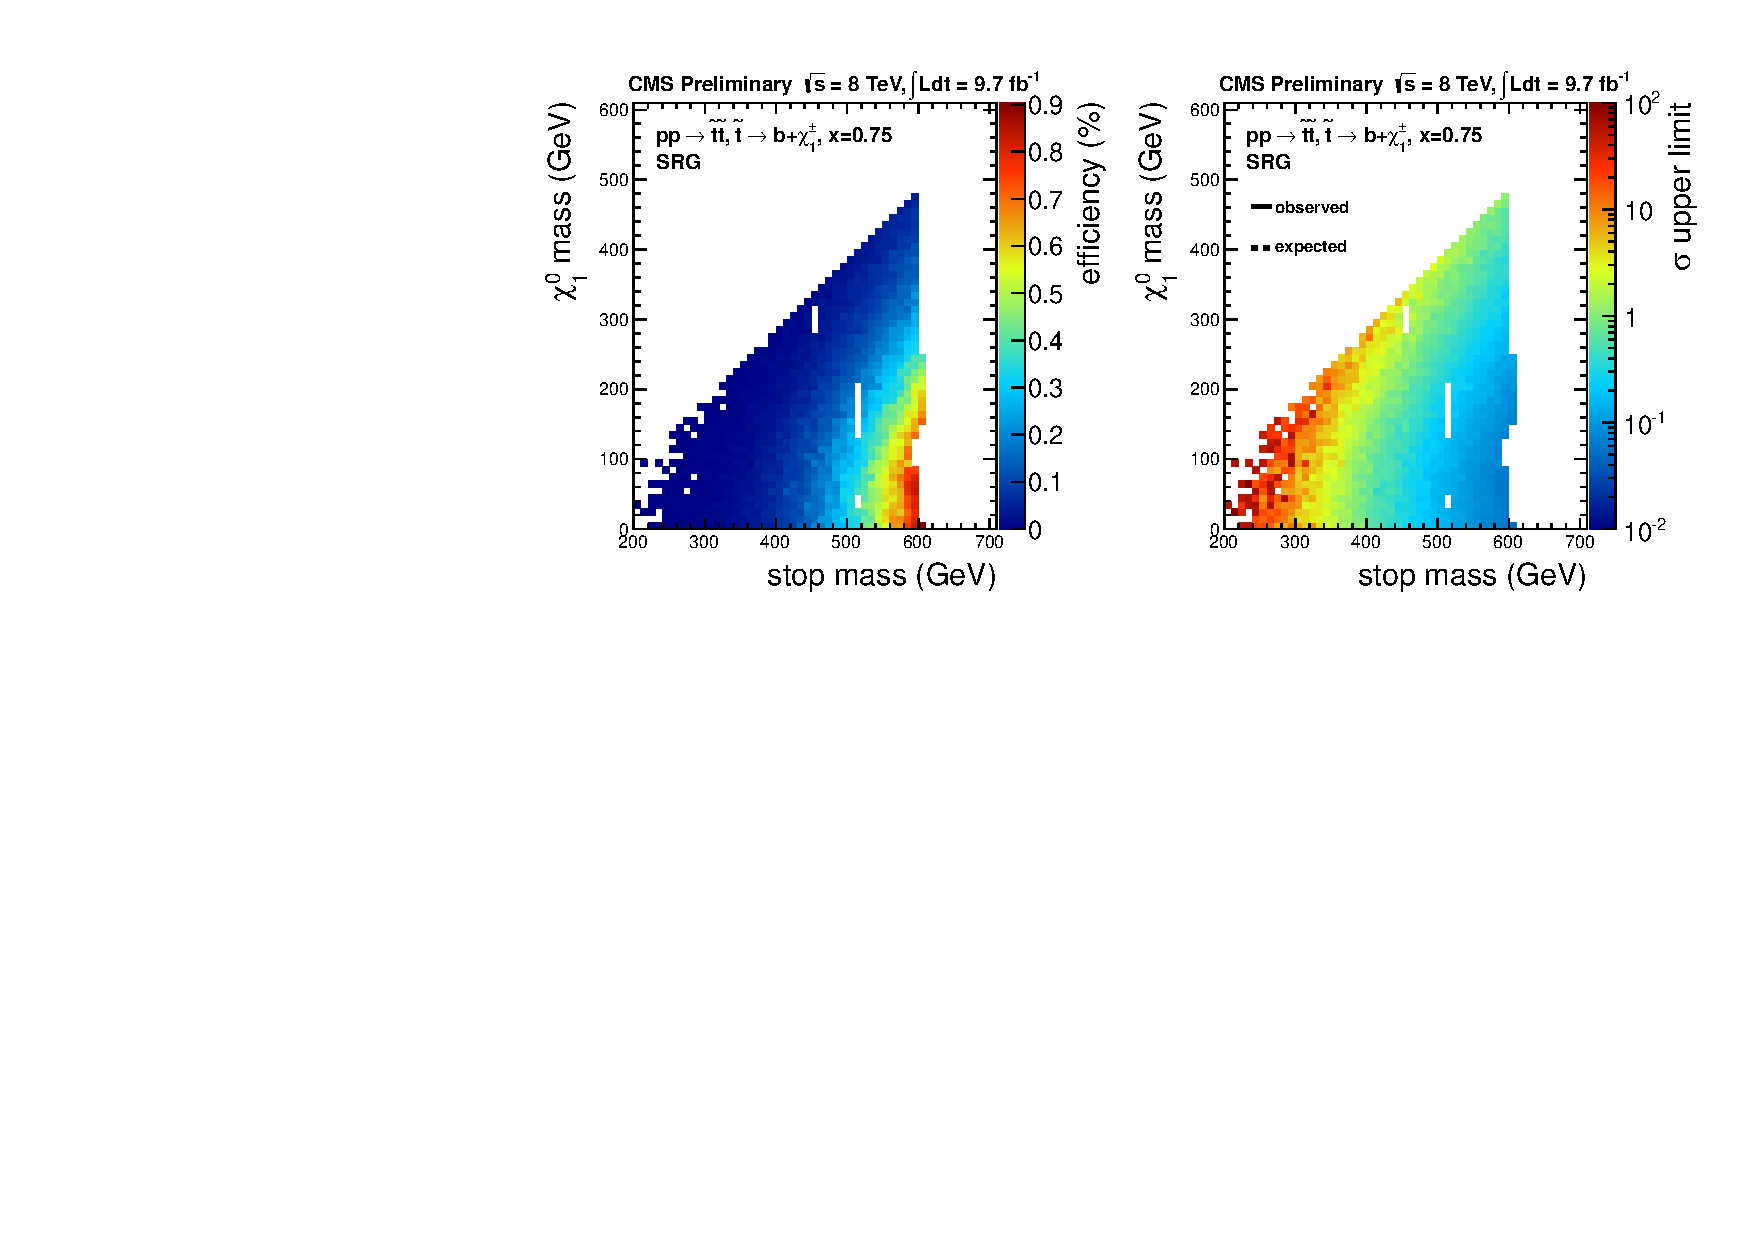
\includegraphics[width=1.\linewidth]{plots/T2bw_x75_SRG.pdf}
    \caption{Signal efficiency (left) and cross section upper limit
      (right) for the T2bw model with x=0.75, showing both the expected and
      observed exclusion contours. The results for signal regions SRF (top),
      and SRG (bottom) are shown separately.}
\label{fig:allsrlimits3T2bw0p75}
      \end{center}
\end{figure}

\begin{figure}[hbt]
  \begin{center}
        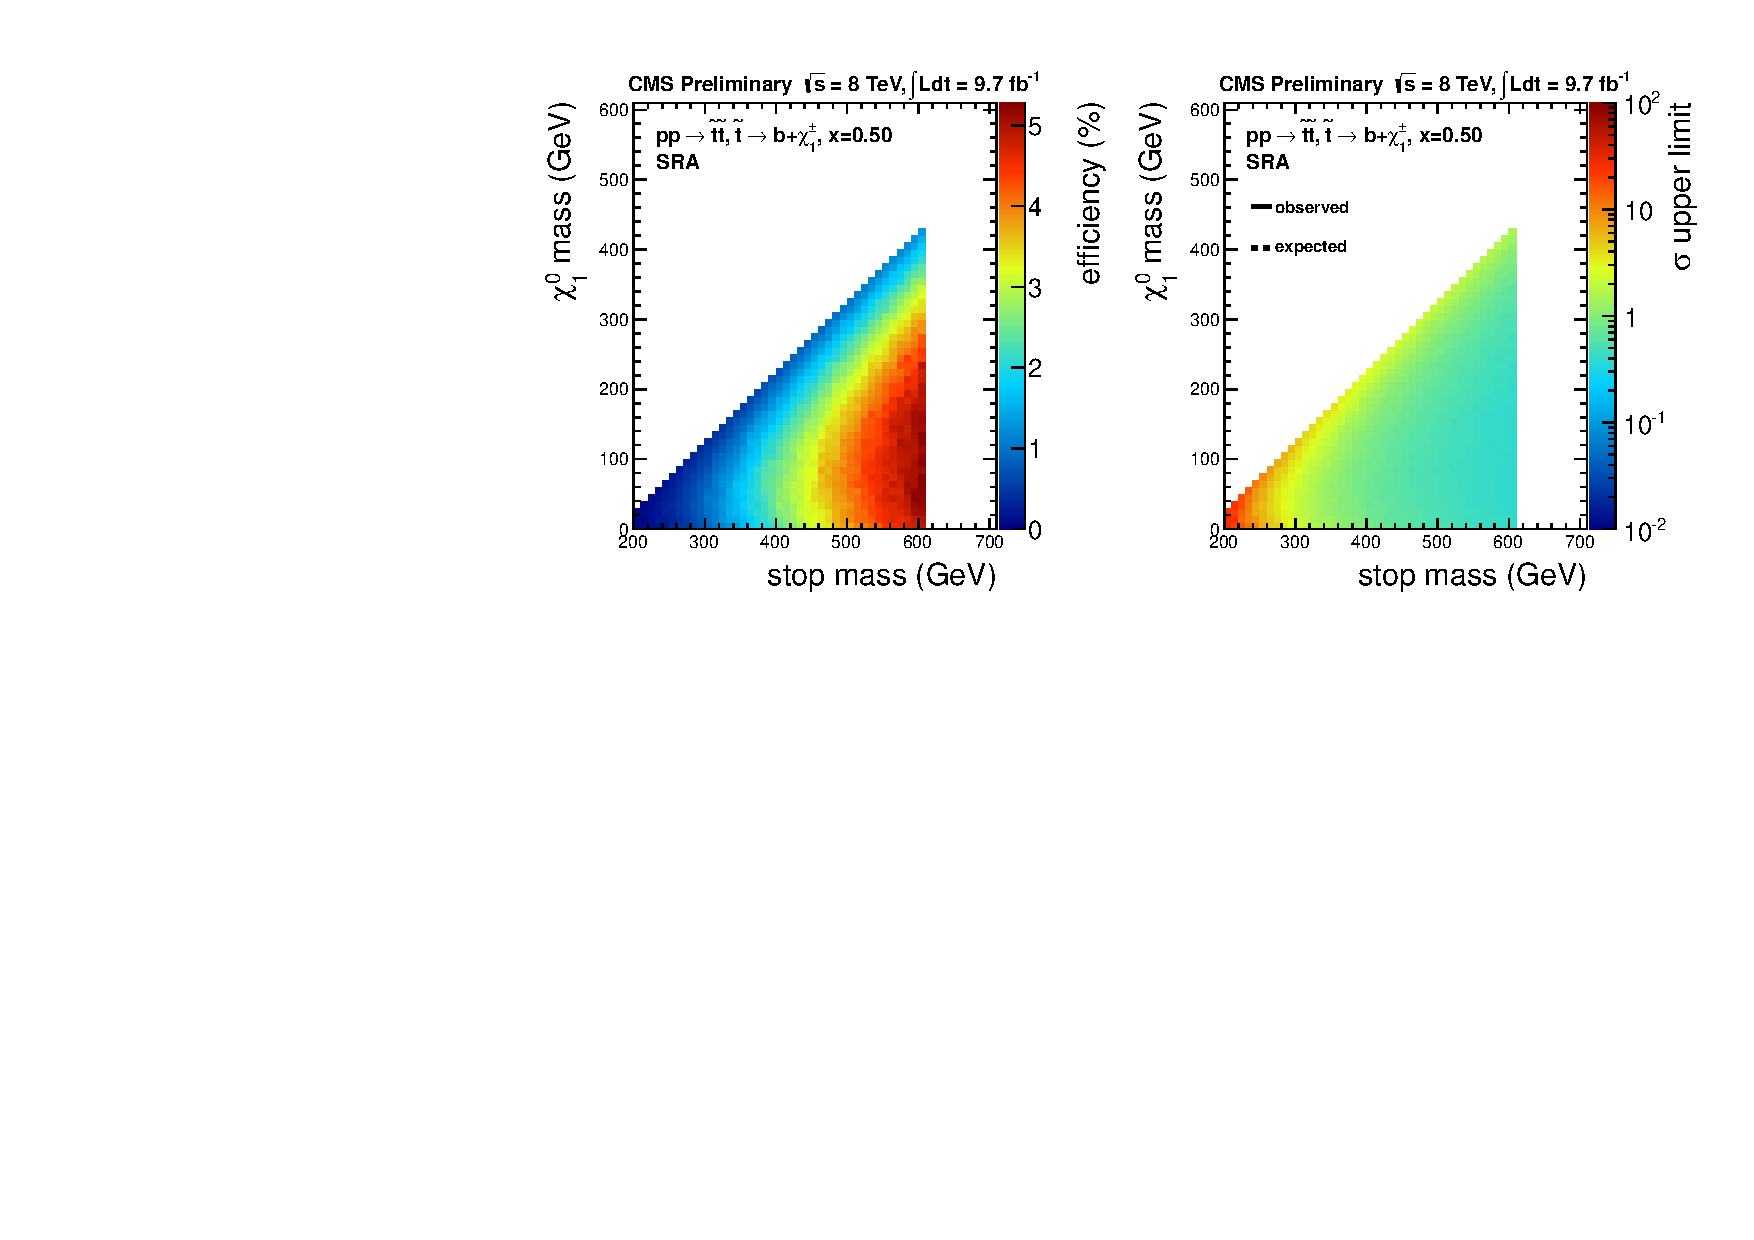
\includegraphics[width=1.\linewidth]{plots/T2bw_x50_SRA.pdf}
        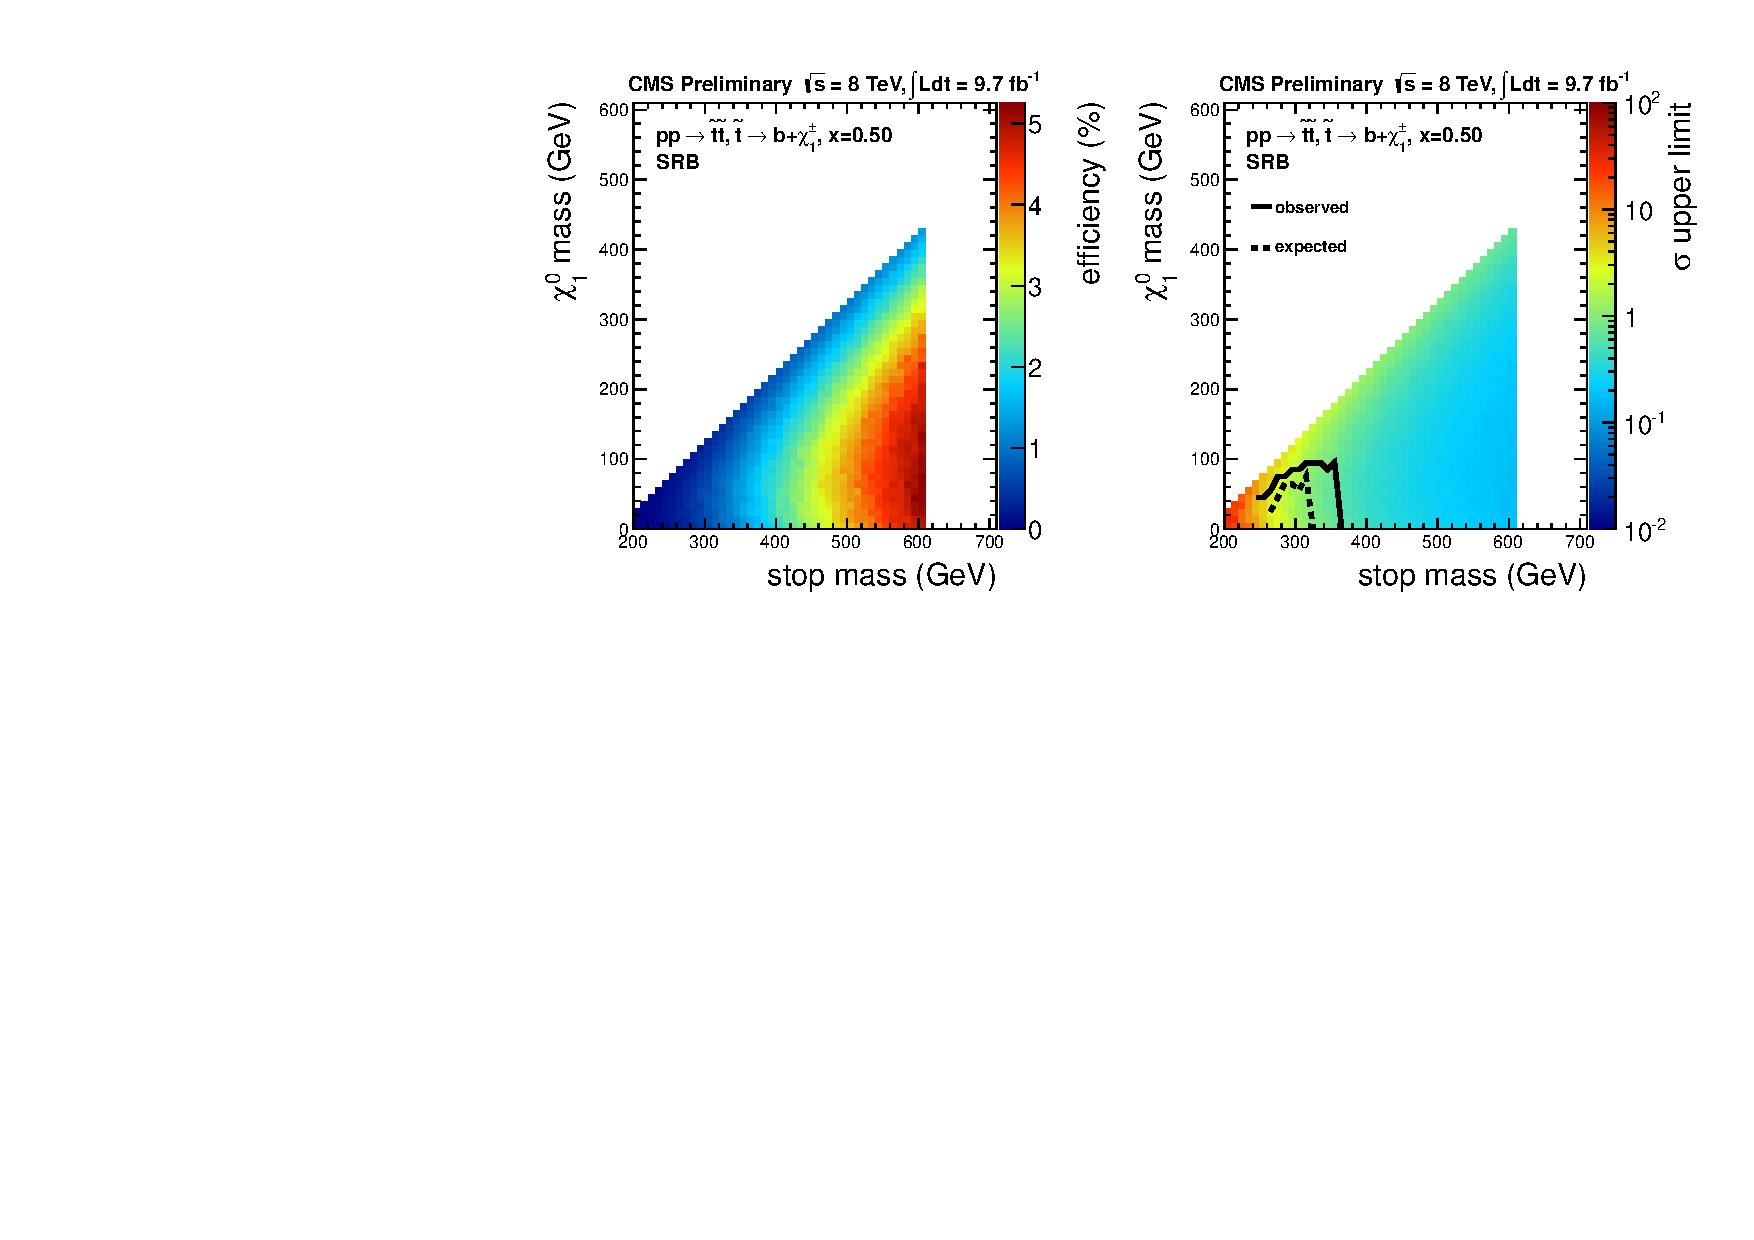
\includegraphics[width=1.\linewidth]{plots/T2bw_x50_SRB.pdf}
        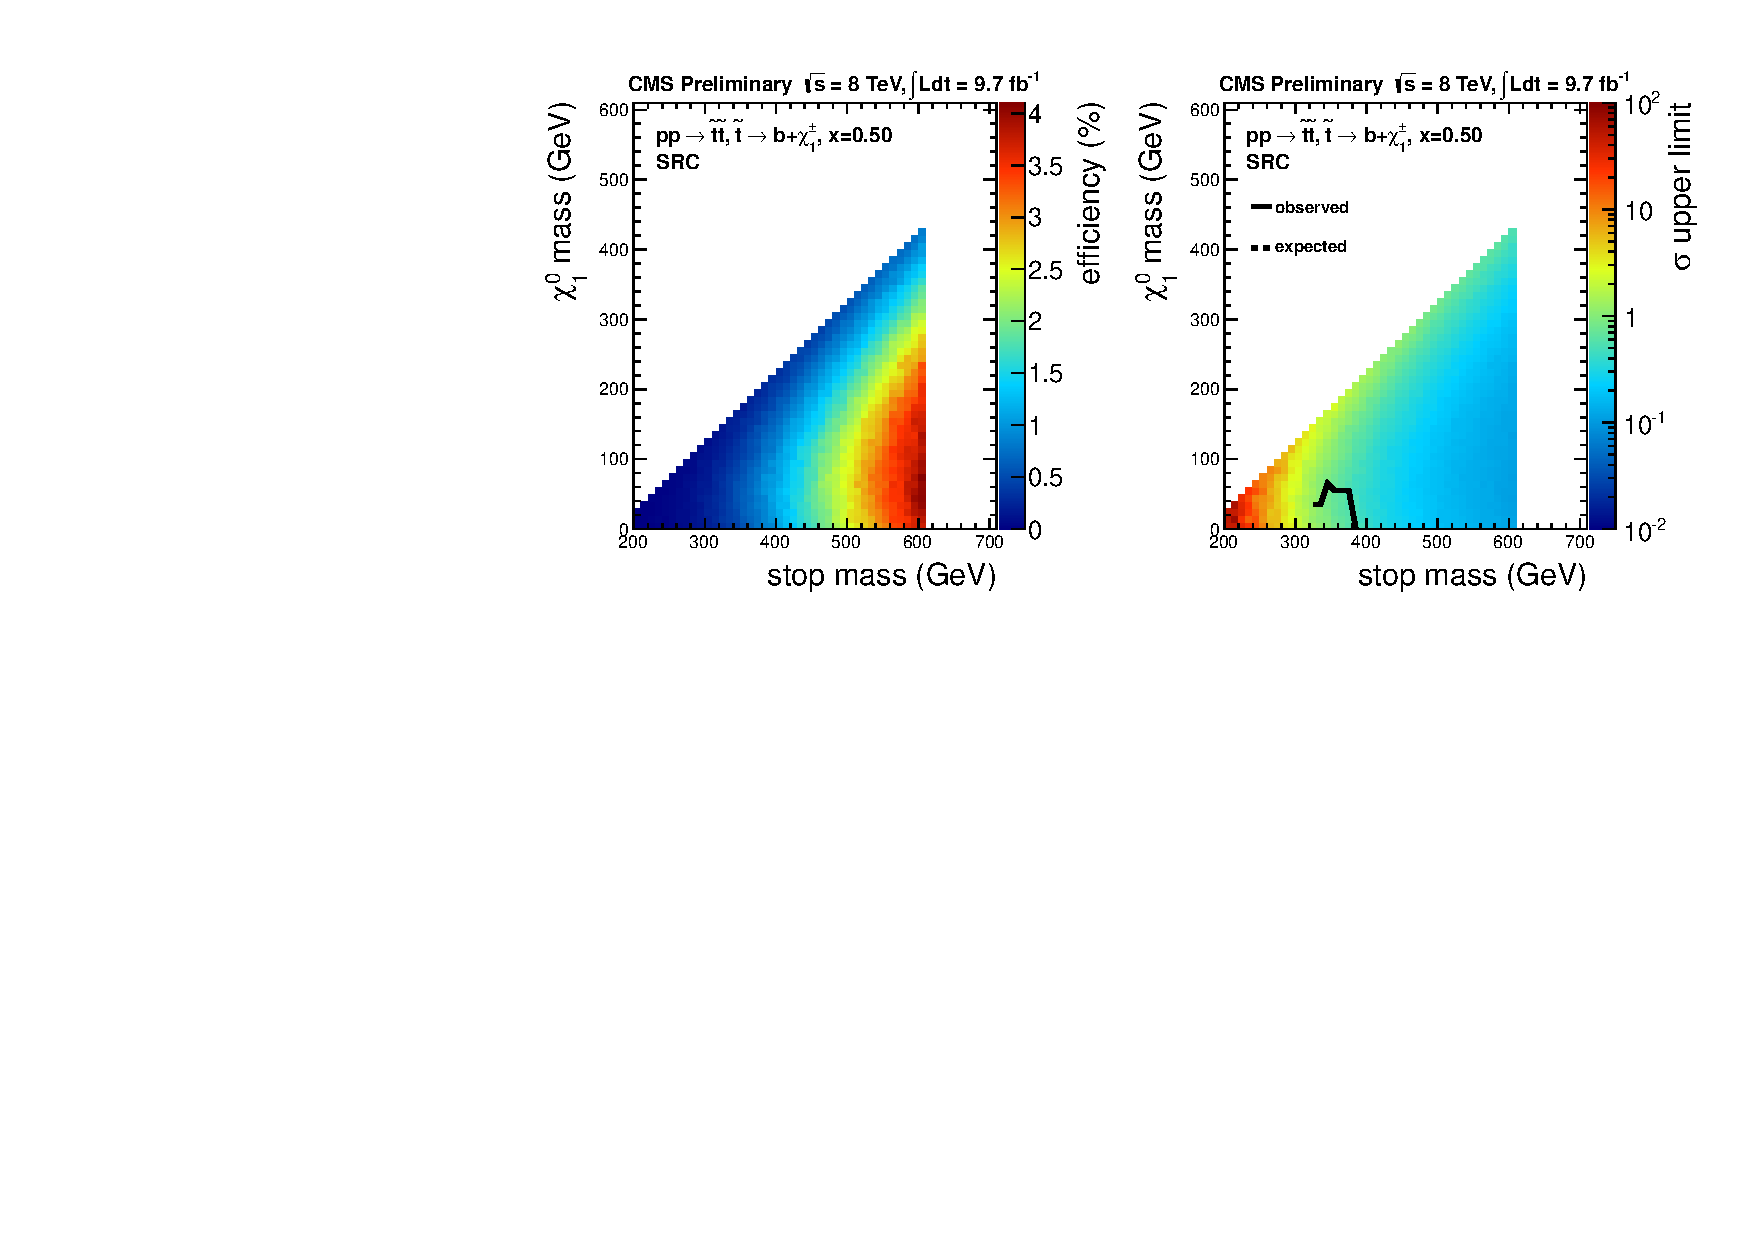
\includegraphics[width=1.\linewidth]{plots/T2bw_x50_SRC.pdf}
    \caption{Signal efficiency (left) and cross section upper limit
      (right) for the T2bw model with x=0.5, showing both the expected and
      observed exclusion contours. The results for signal regions SRA (top),
      SRB (middle) and SRC (bottom) are shown separately.}
\label{fig:allsrlimitsT2bw0p5}
      \end{center}
\end{figure}

\begin{figure}[hbt]
  \begin{center}
        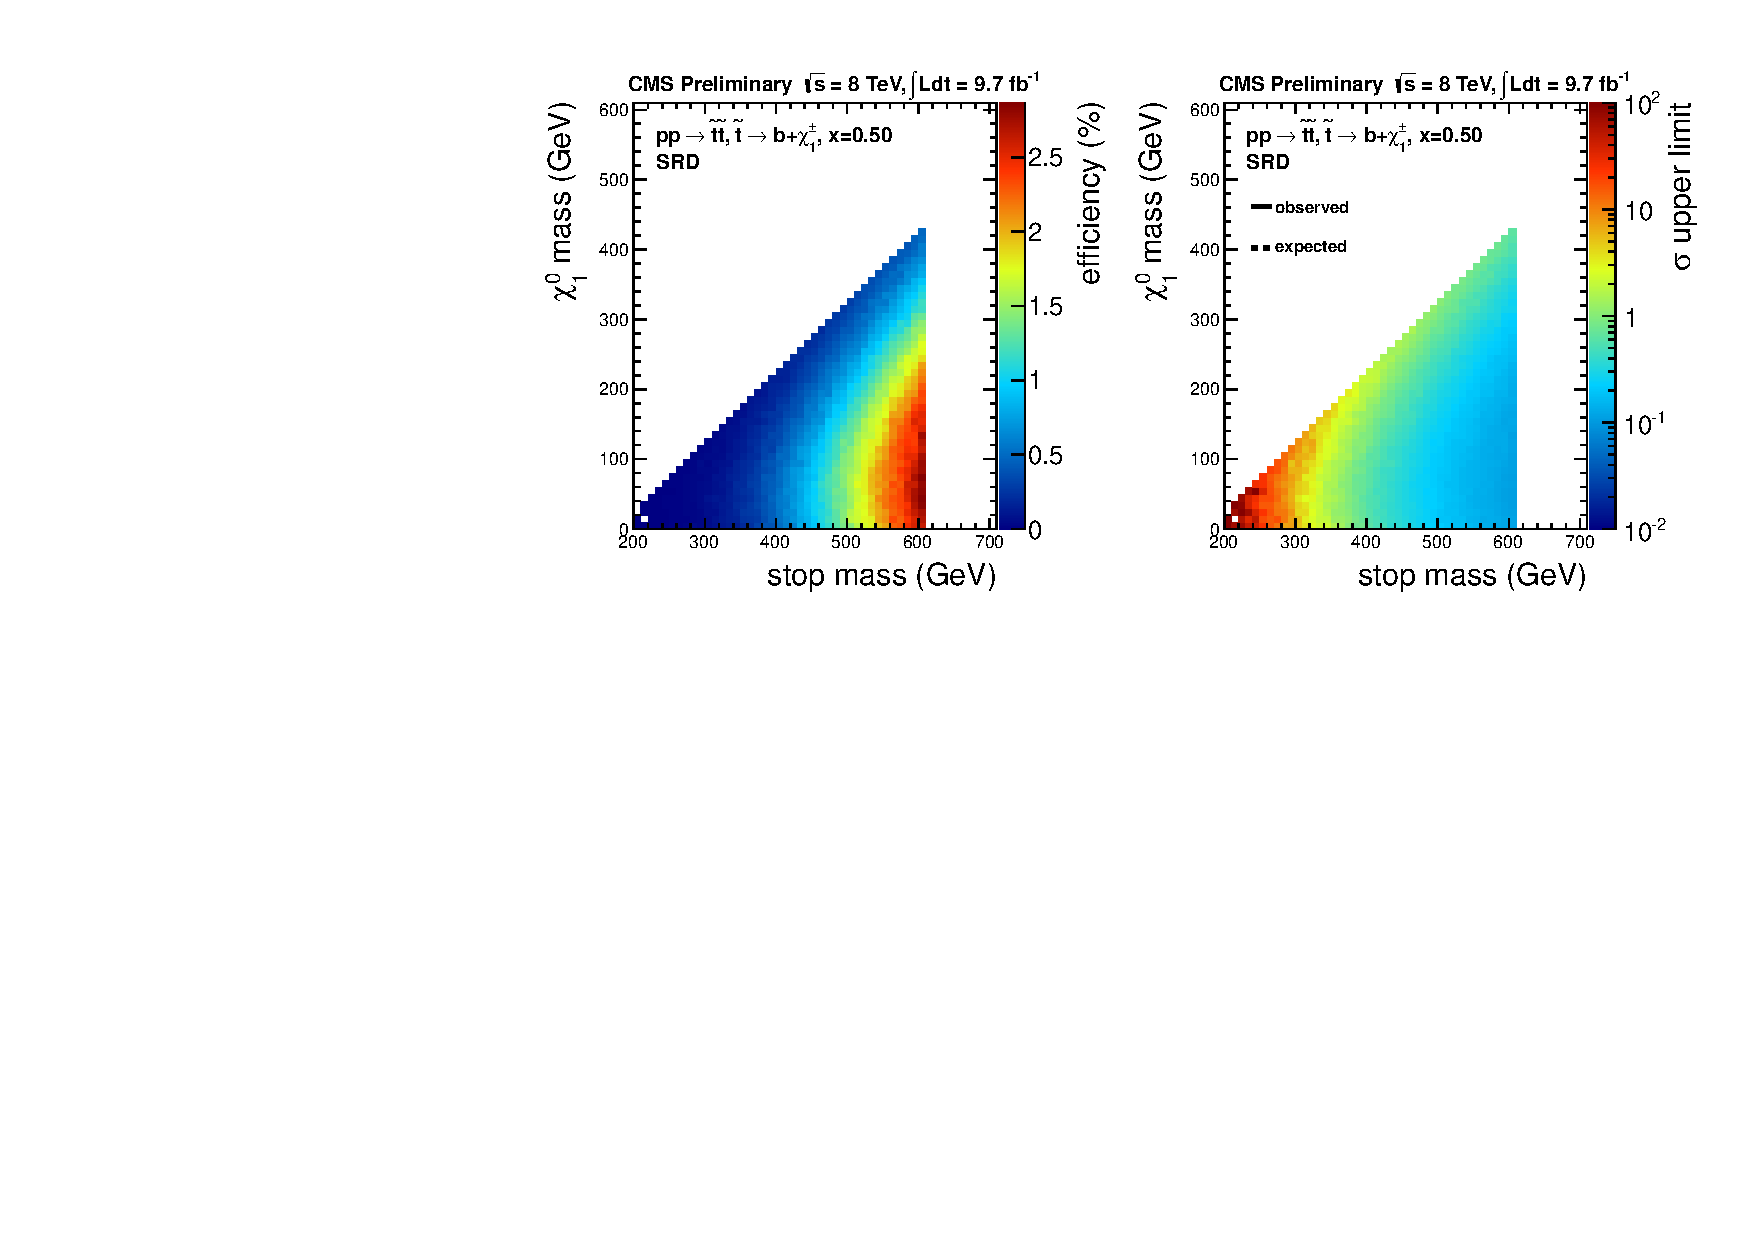
\includegraphics[width=1.\linewidth]{plots/T2bw_x50_SRD.pdf}
        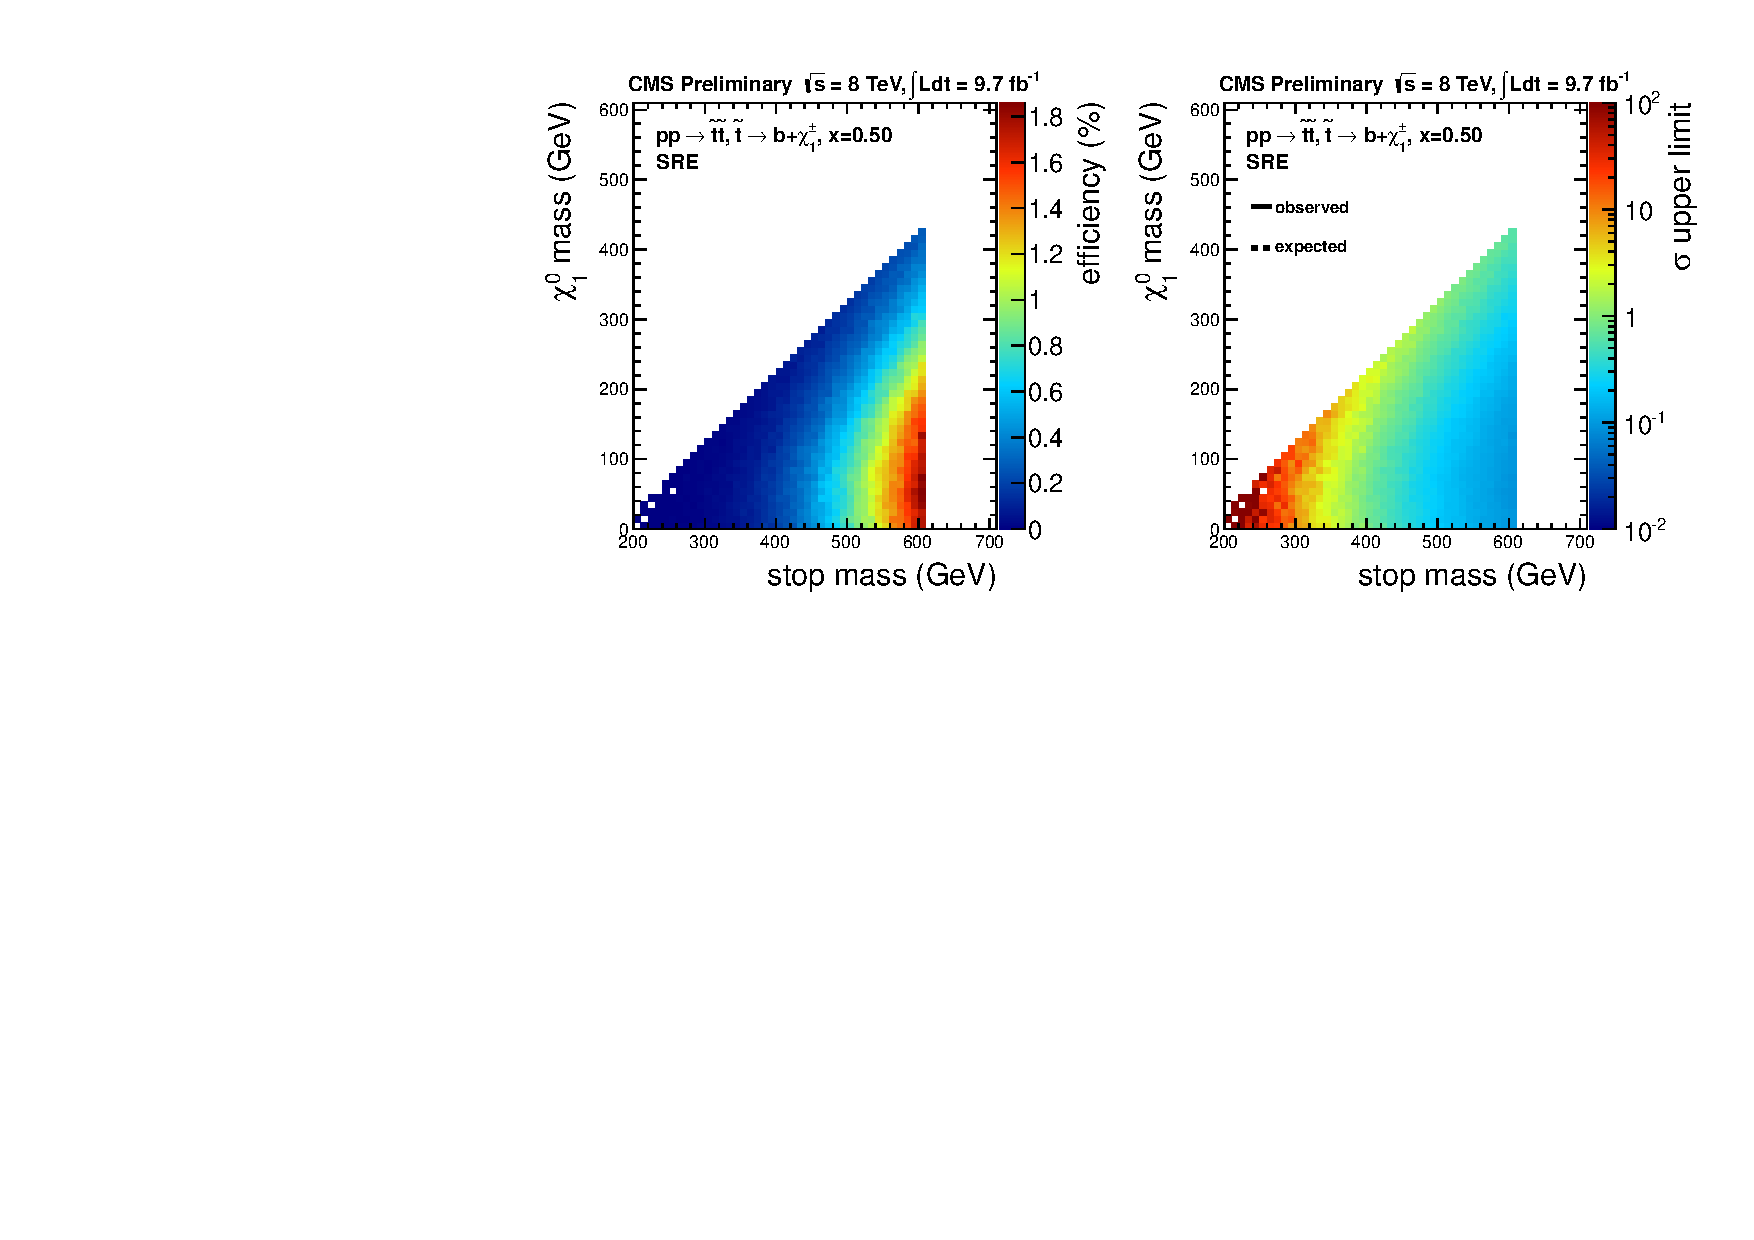
\includegraphics[width=1.\linewidth]{plots/T2bw_x50_SRE.pdf}
    \caption{Signal efficiency (left) and cross section upper limit
      (right) for the T2bw model with x=0.5, showing both the expected and
      observed exclusion contours. The results for signal regions SRD (top),
      and SRE (bottom) are shown separately.}
\label{fig:allsrlimits2T2bw0p5}
      \end{center}
\end{figure}

\begin{figure}[hbt]
  \begin{center}
        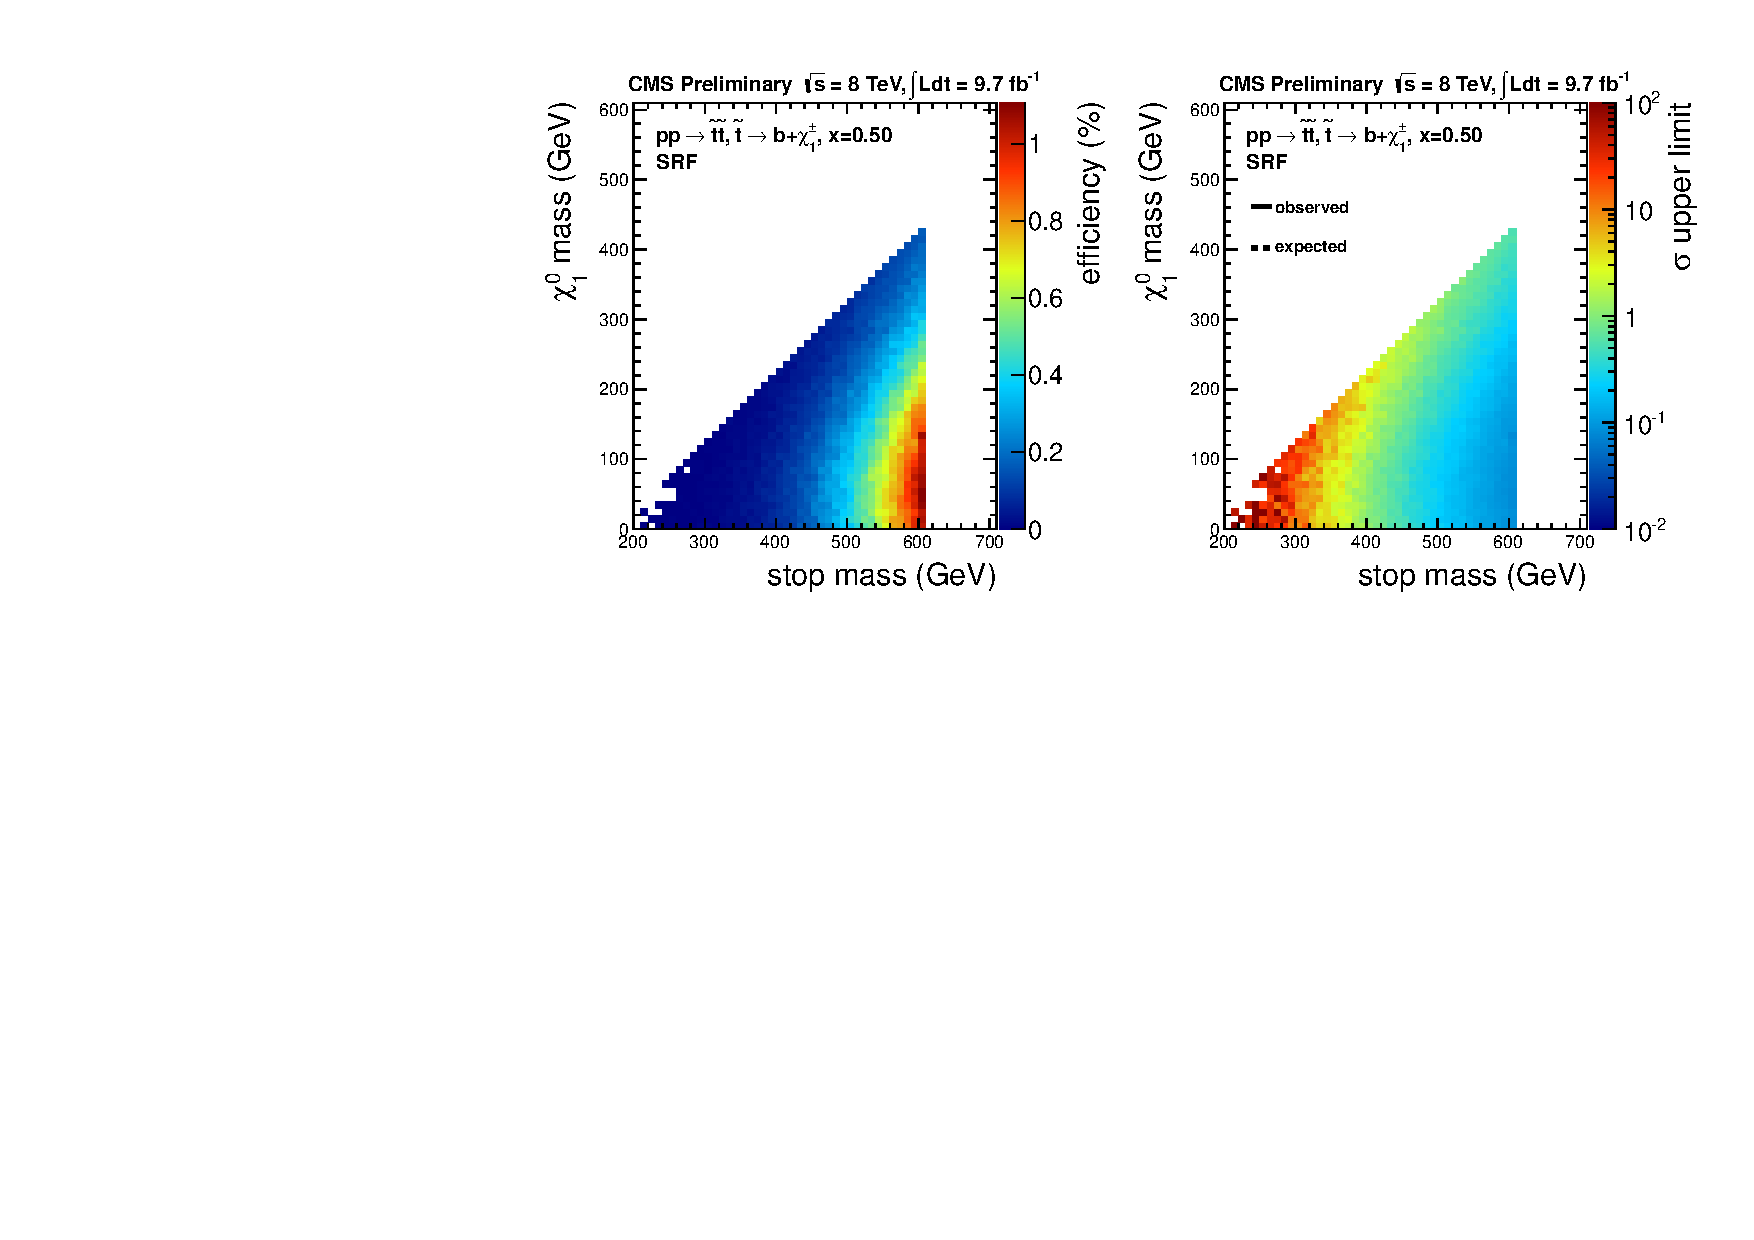
\includegraphics[width=1.\linewidth]{plots/T2bw_x50_SRF.pdf}
        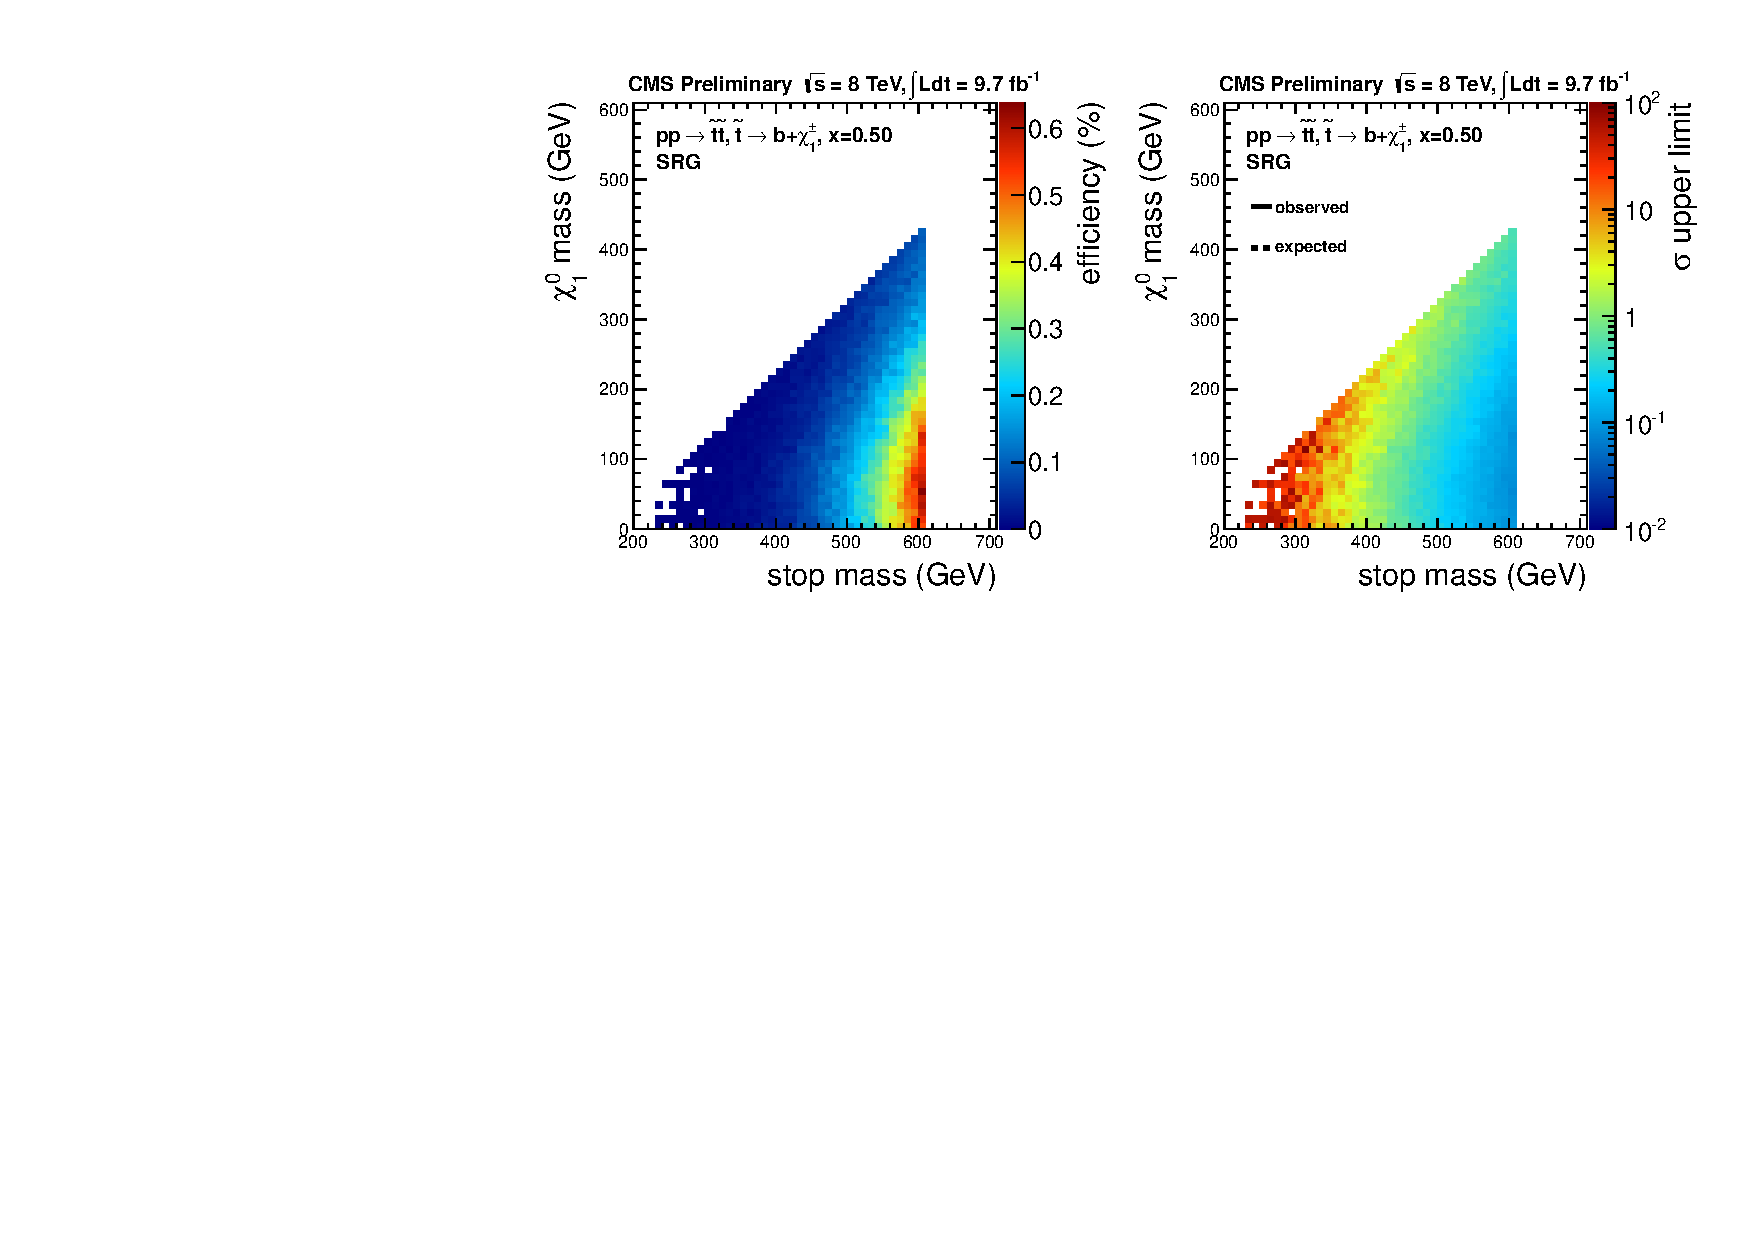
\includegraphics[width=1.\linewidth]{plots/T2bw_x50_SRG.pdf}
    \caption{Signal efficiency (left) and cross section upper limit
      (right) for the T2bw model with x=0.5, showing both the expected and
      observed exclusion contours. The results for signal regions SRF (top),
      and SRG (bottom) are shown separately.}
\label{fig:allsrlimits3T2bw0p5}
      \end{center}
\end{figure}


A combined result is obtained using the observed limit from the signal
region with the best expected limit for each scan point. The combined cross
section upper limits, with the observed and expected exclusion contours, are
shown in Figure~\ref{fig:comblimit} for T2tt and 
Figure~\ref{fig:comblimitT2bw} for T2bw (left).
%The combination is performed by selecting at each scan point the
%observed limit from the signal region with the best expected limit.
The signal region with the best expected limit for each scan point is
also shown in Figure~\ref{fig:comblimit} for T2tt and 
Figure~\ref{fig:comblimitT2bw} for T2bw (right). 
For the T2tt scenario, these results exclude stops with masses
in the range of approximately $230-460$ GeV, for LSP masses up to about
$130$ GeV. In the T2bw scenario with x=0.75, this search excludes
stops with masses in the range of approximately $150-430$ GeV, for LSP
masses up to about $140$ GeV. The sensitivity is reduced in the
x=0.5 scenario, where the results exclude stops with masses in the
range of approximately $250-360$ GeV, for LSP masses less than
approximately $100$ GeV.

 \begin{figure}[hbt]
  \begin{center}
       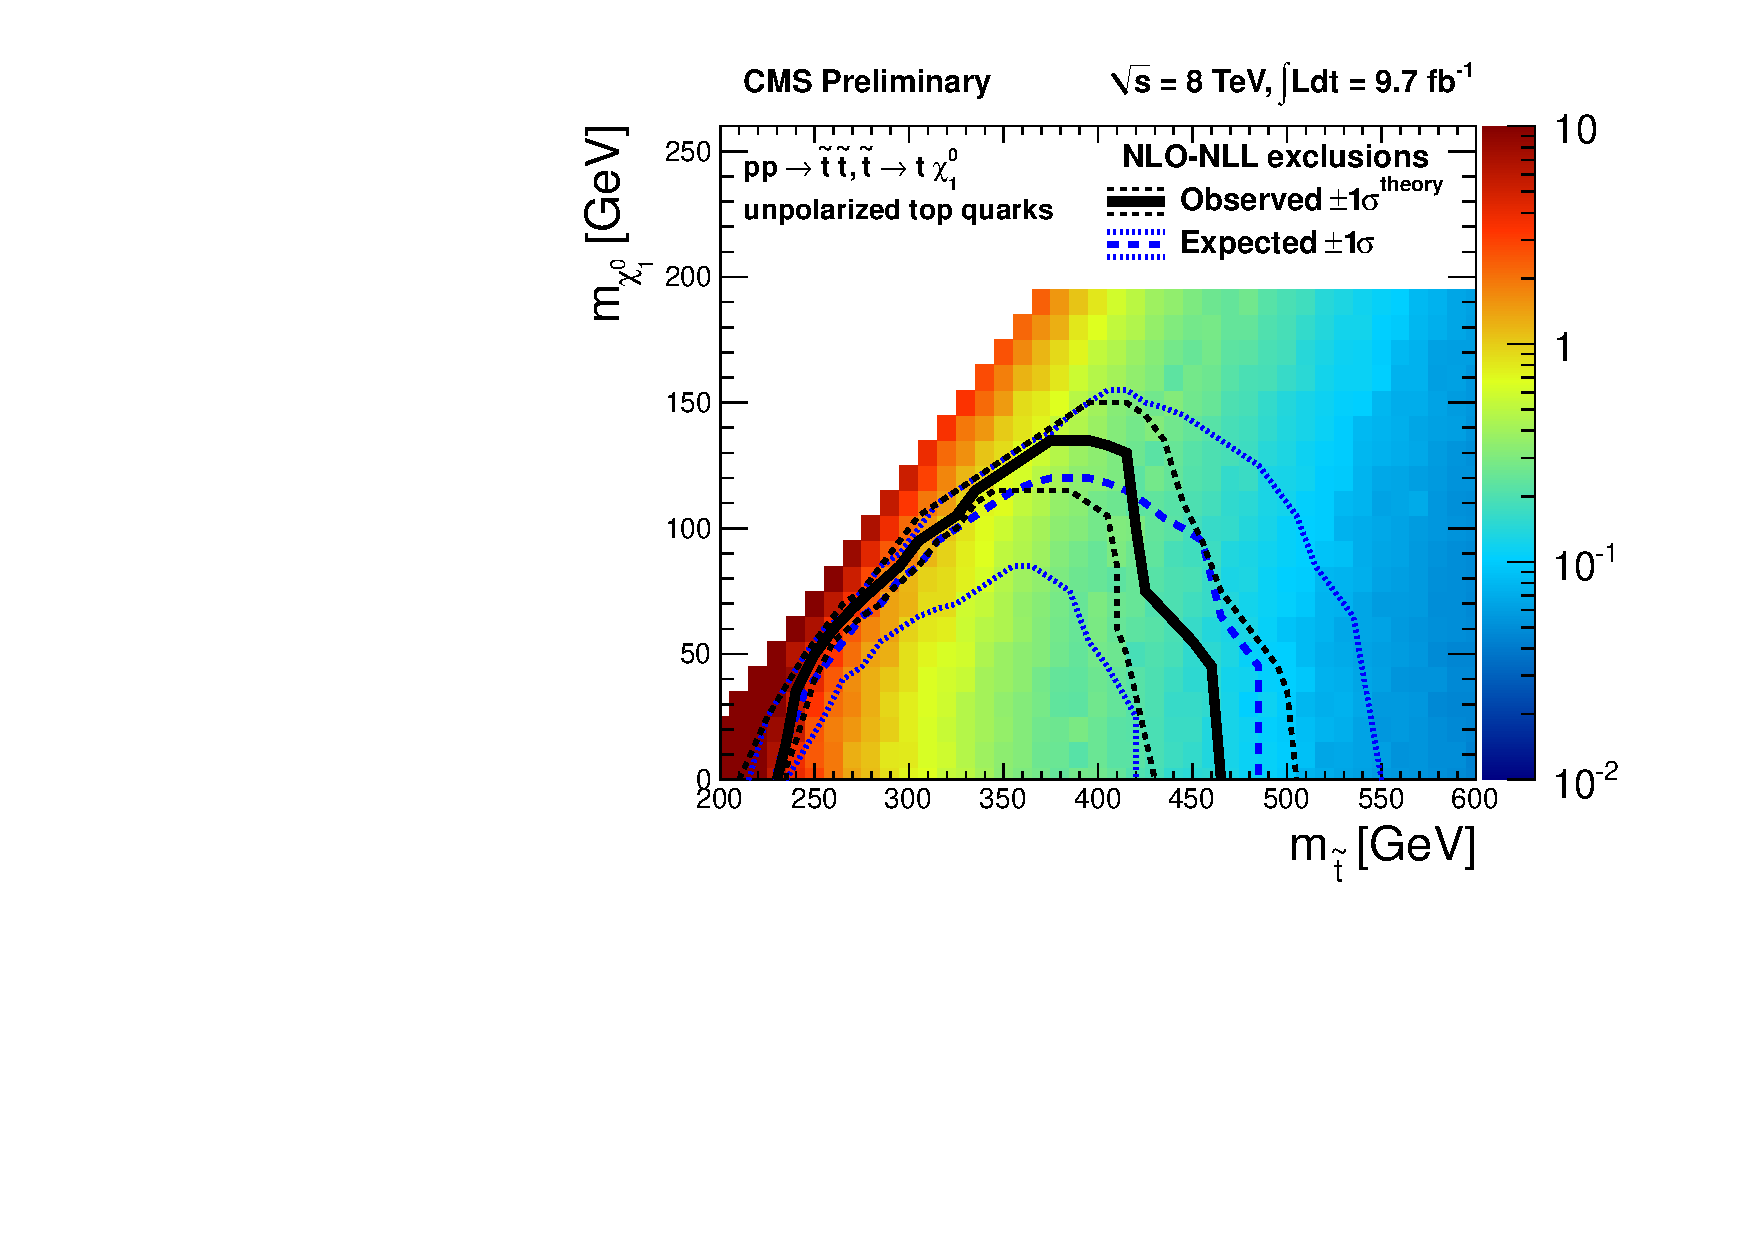
\includegraphics[height=6.5cm]{plots/combinePlots_T2tt.pdf}%
       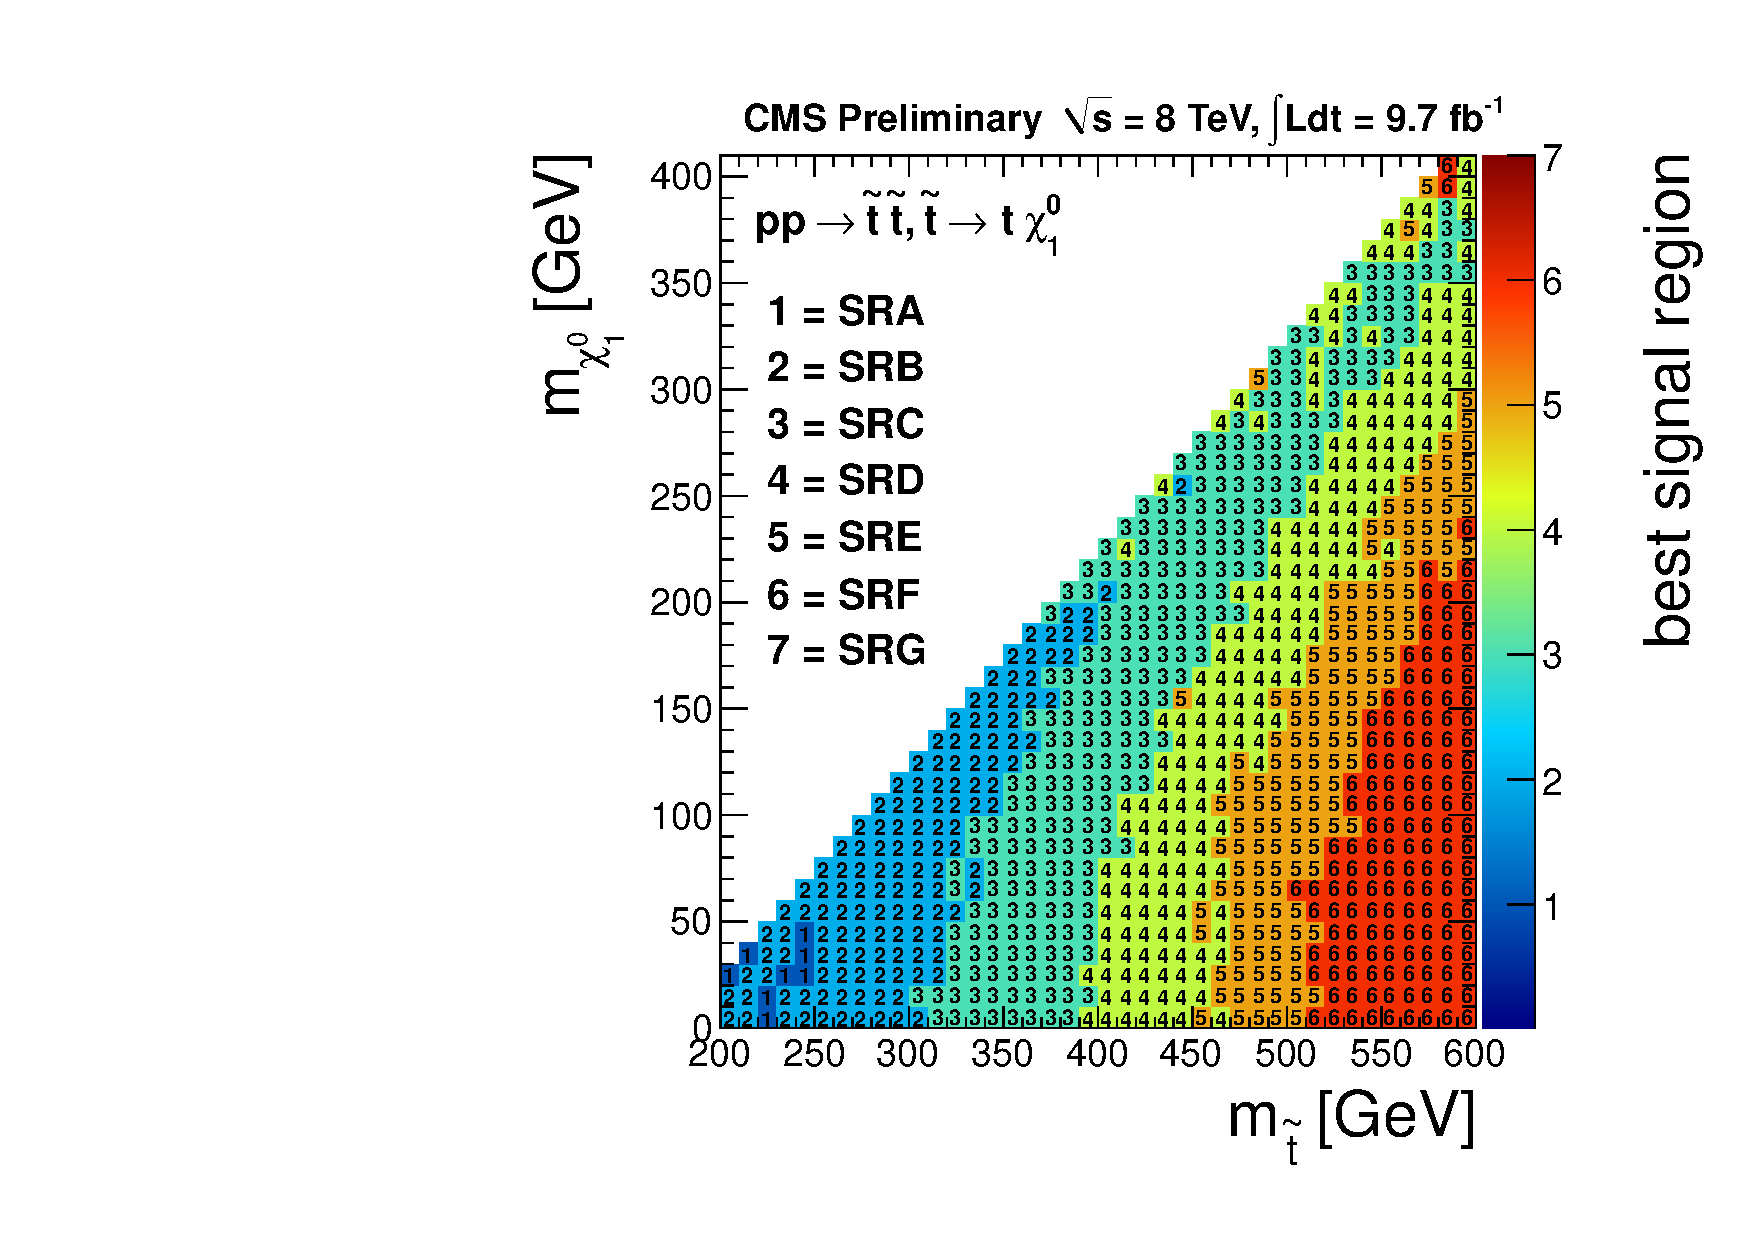
\includegraphics[height=6.5cm]{plots/combinePlots_T2tt_bestSignalRegion.pdf}
    \caption{Upper limit on the cross section for the T2tt model in
      the plane of stop vs. LSP mass, showing
      both the expected (dashed) and observed (solid curve) exclusion
      contours (left). The observed
      limit is selected from the signal region with the best expected
      limit (shown on right). All uncertainties are included and the
      dotted contours around the dashed expected limit correspond to
      the $\pm 1\sigma$ result.}
\label{fig:comblimit}
      \end{center}
\end{figure}

 \begin{figure}[hbt]
  \begin{center}
       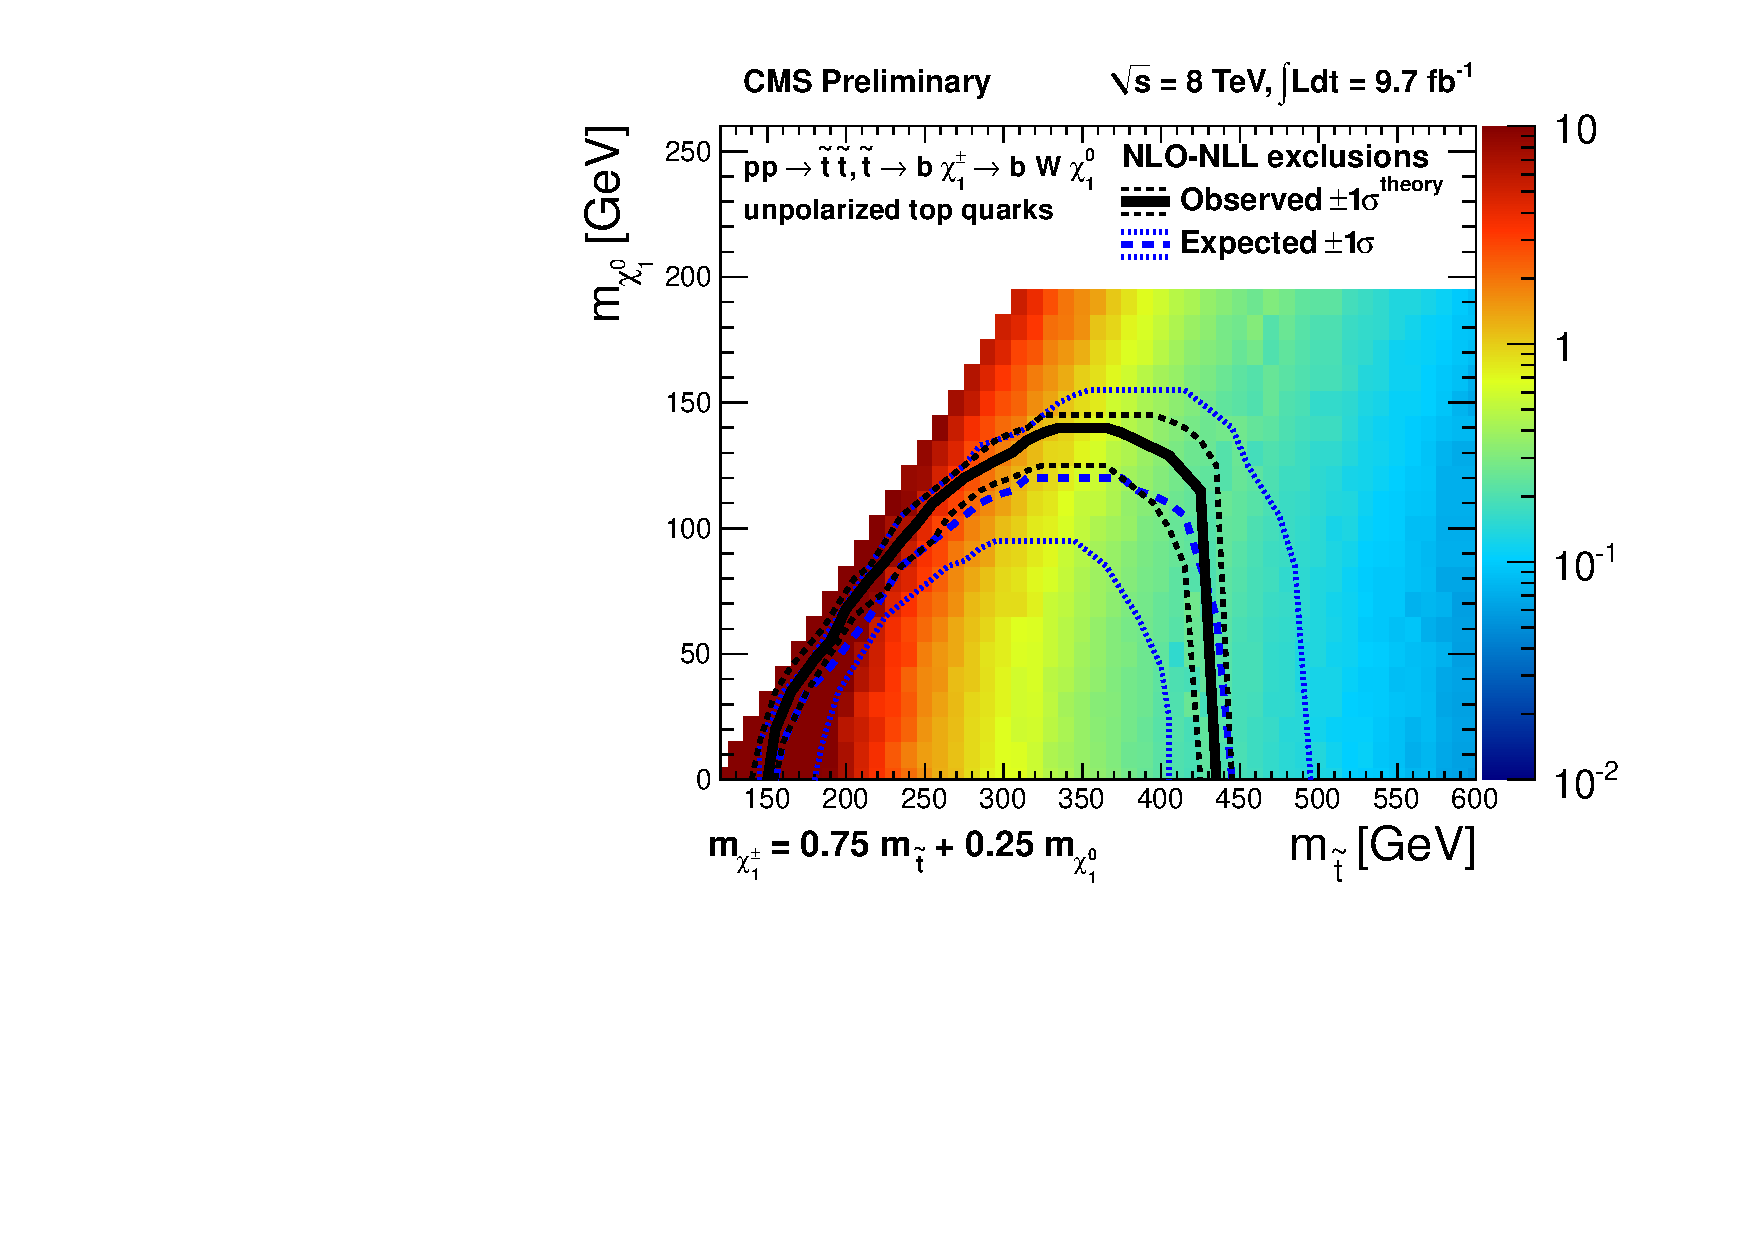
\includegraphics[height=6.5cm]{plots/combinePlots_T2bw_x75.pdf}%
       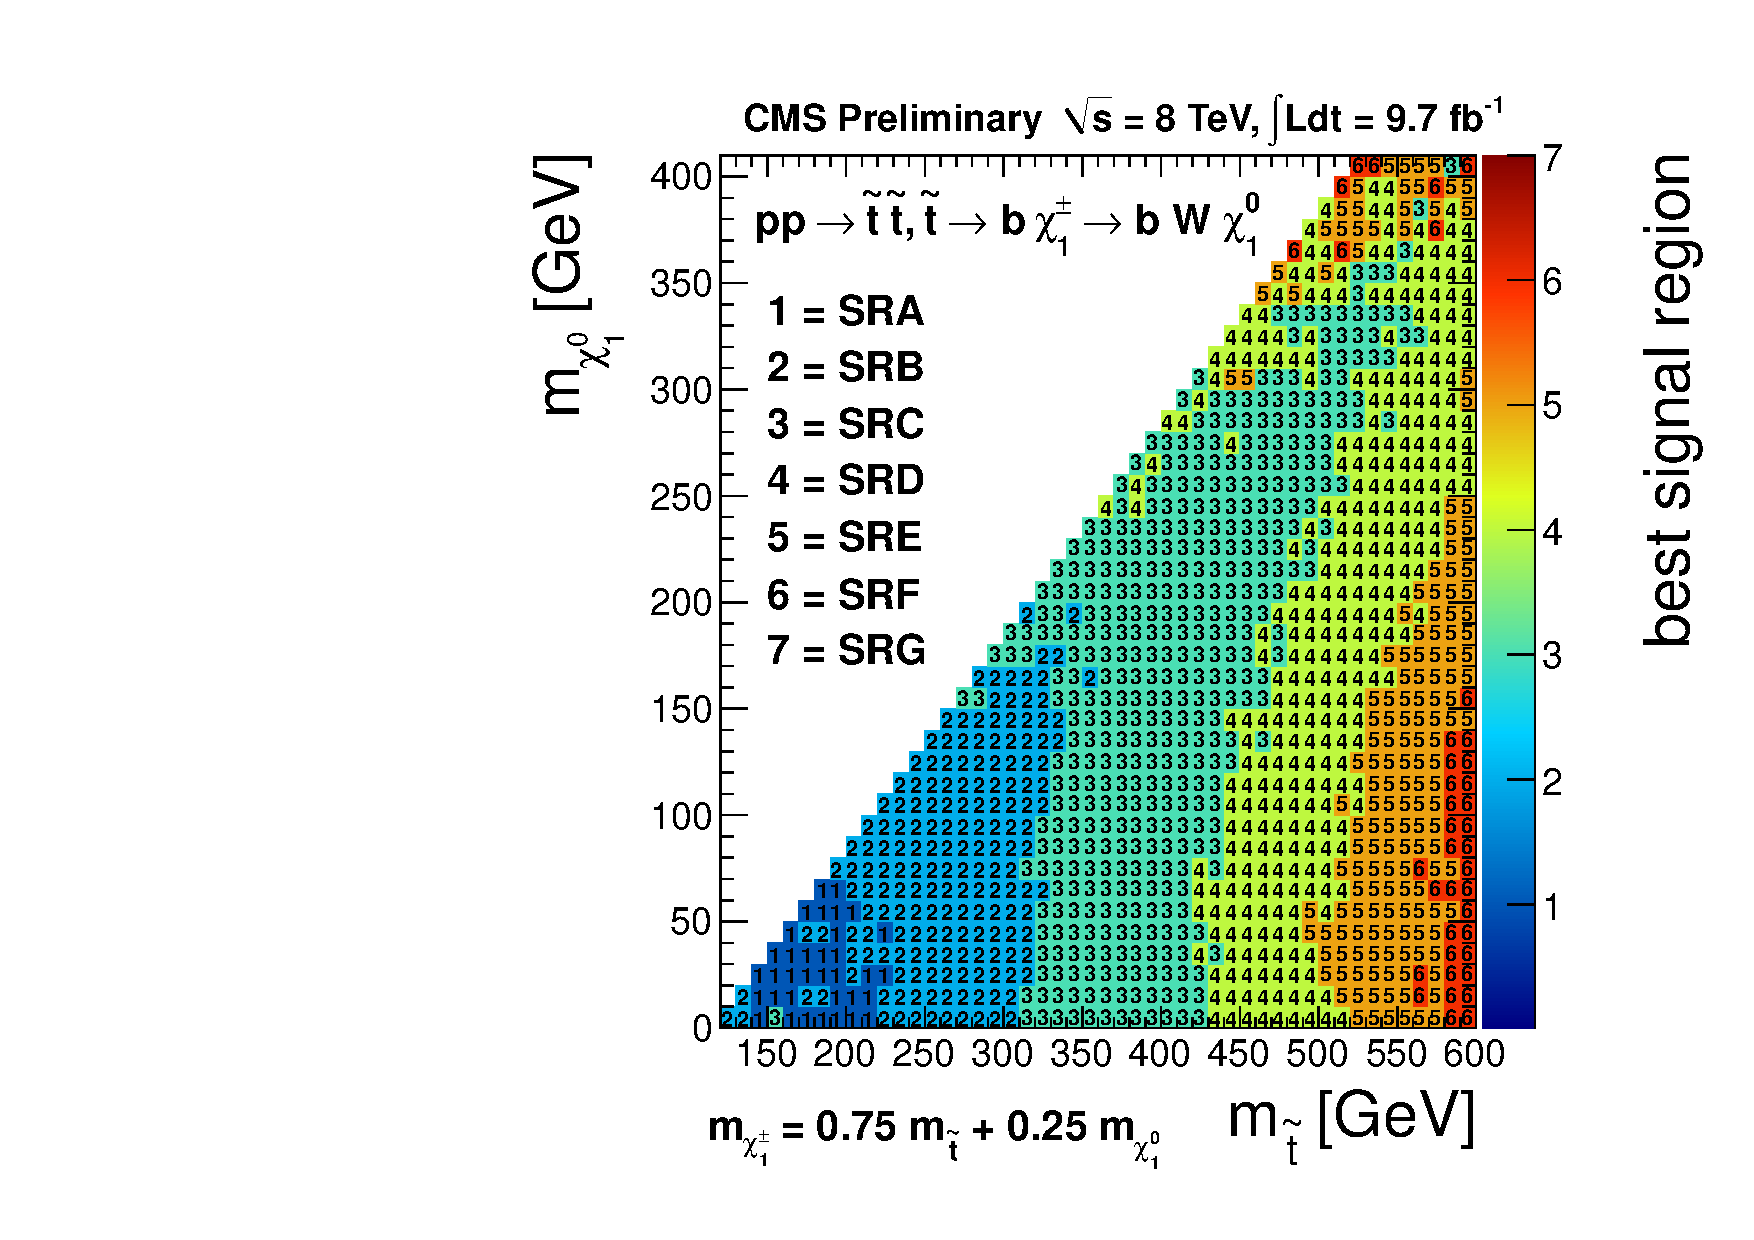
\includegraphics[height=6.5cm]{plots/combinePlots_T2bw_x75_bestSignalRegion.pdf}
       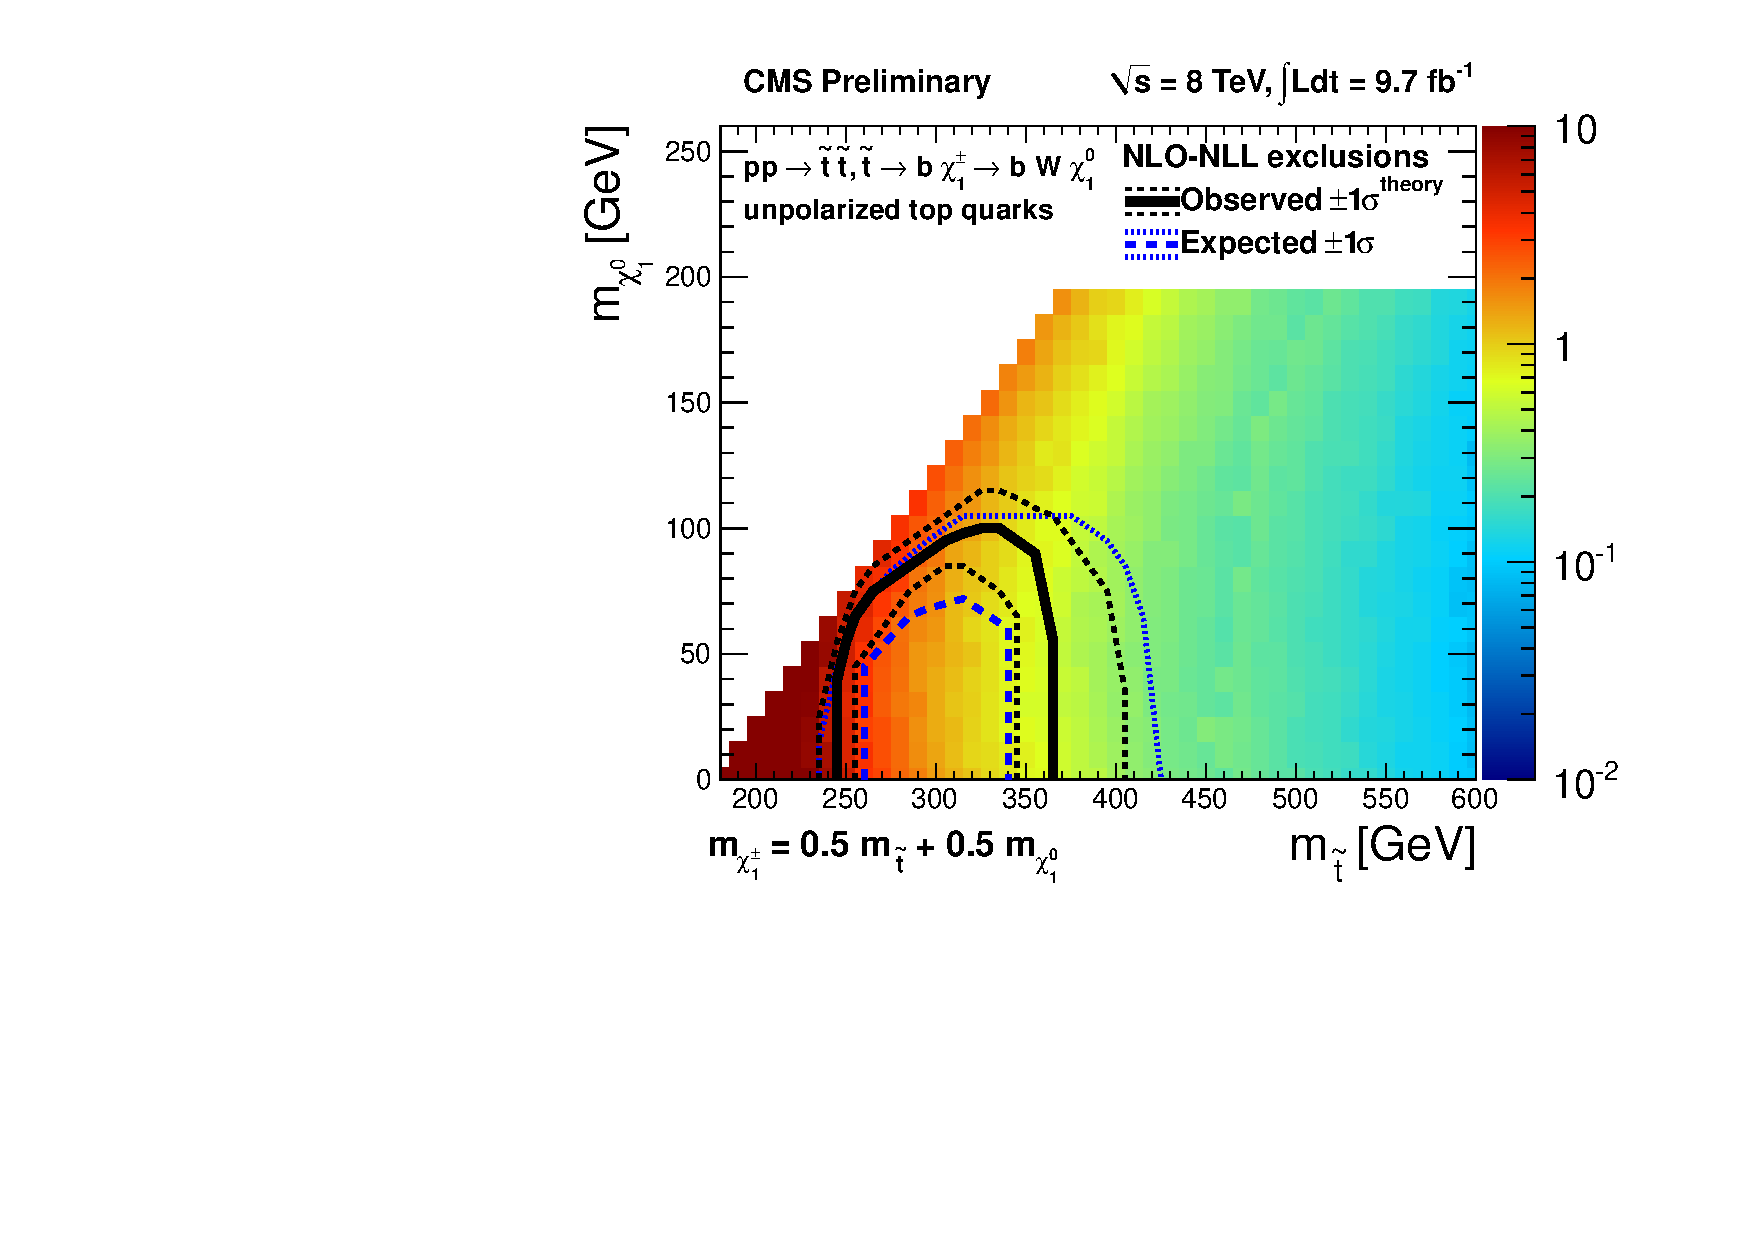
\includegraphics[height=6.5cm]{plots/combinePlots_T2bw_x50.pdf}%
       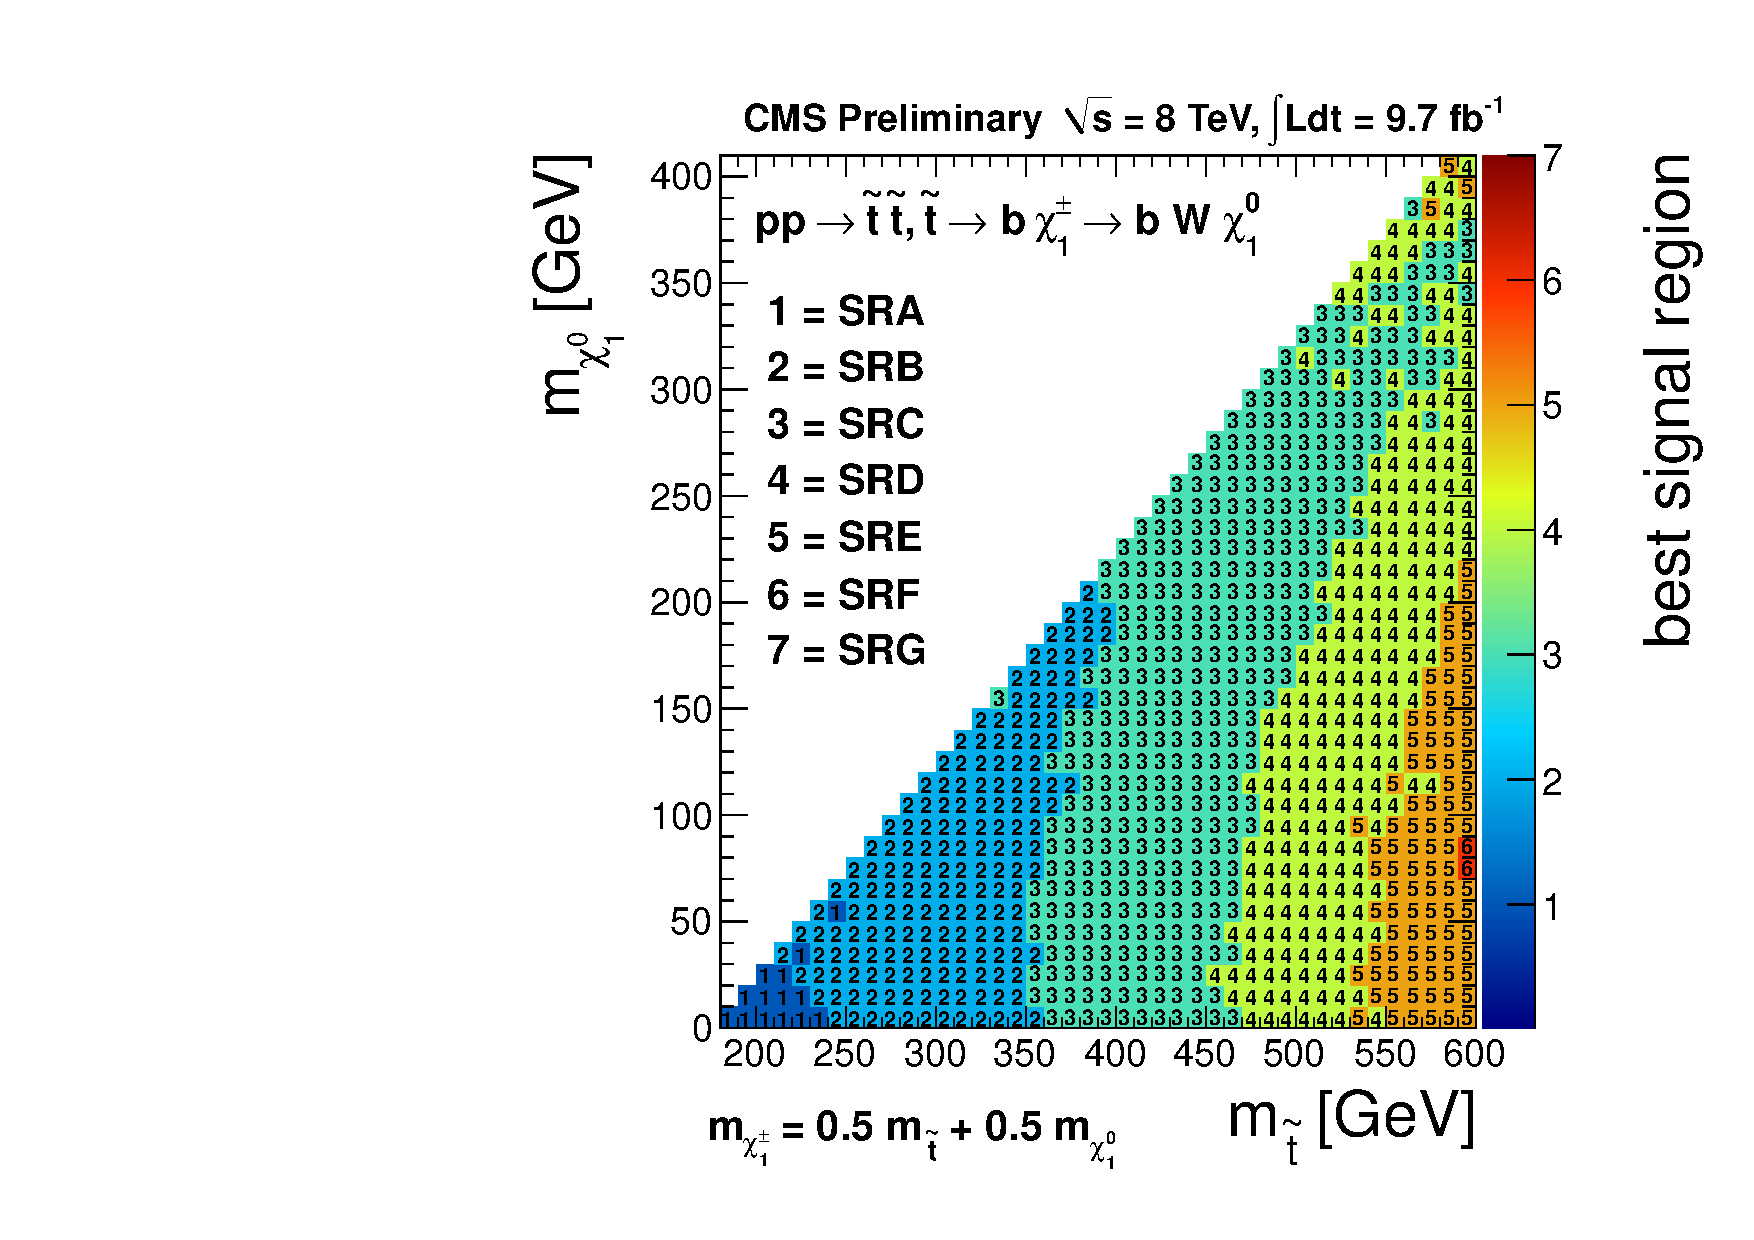
\includegraphics[height=6.5cm]{plots/combinePlots_T2bw_x50_bestSignalRegion.pdf}
       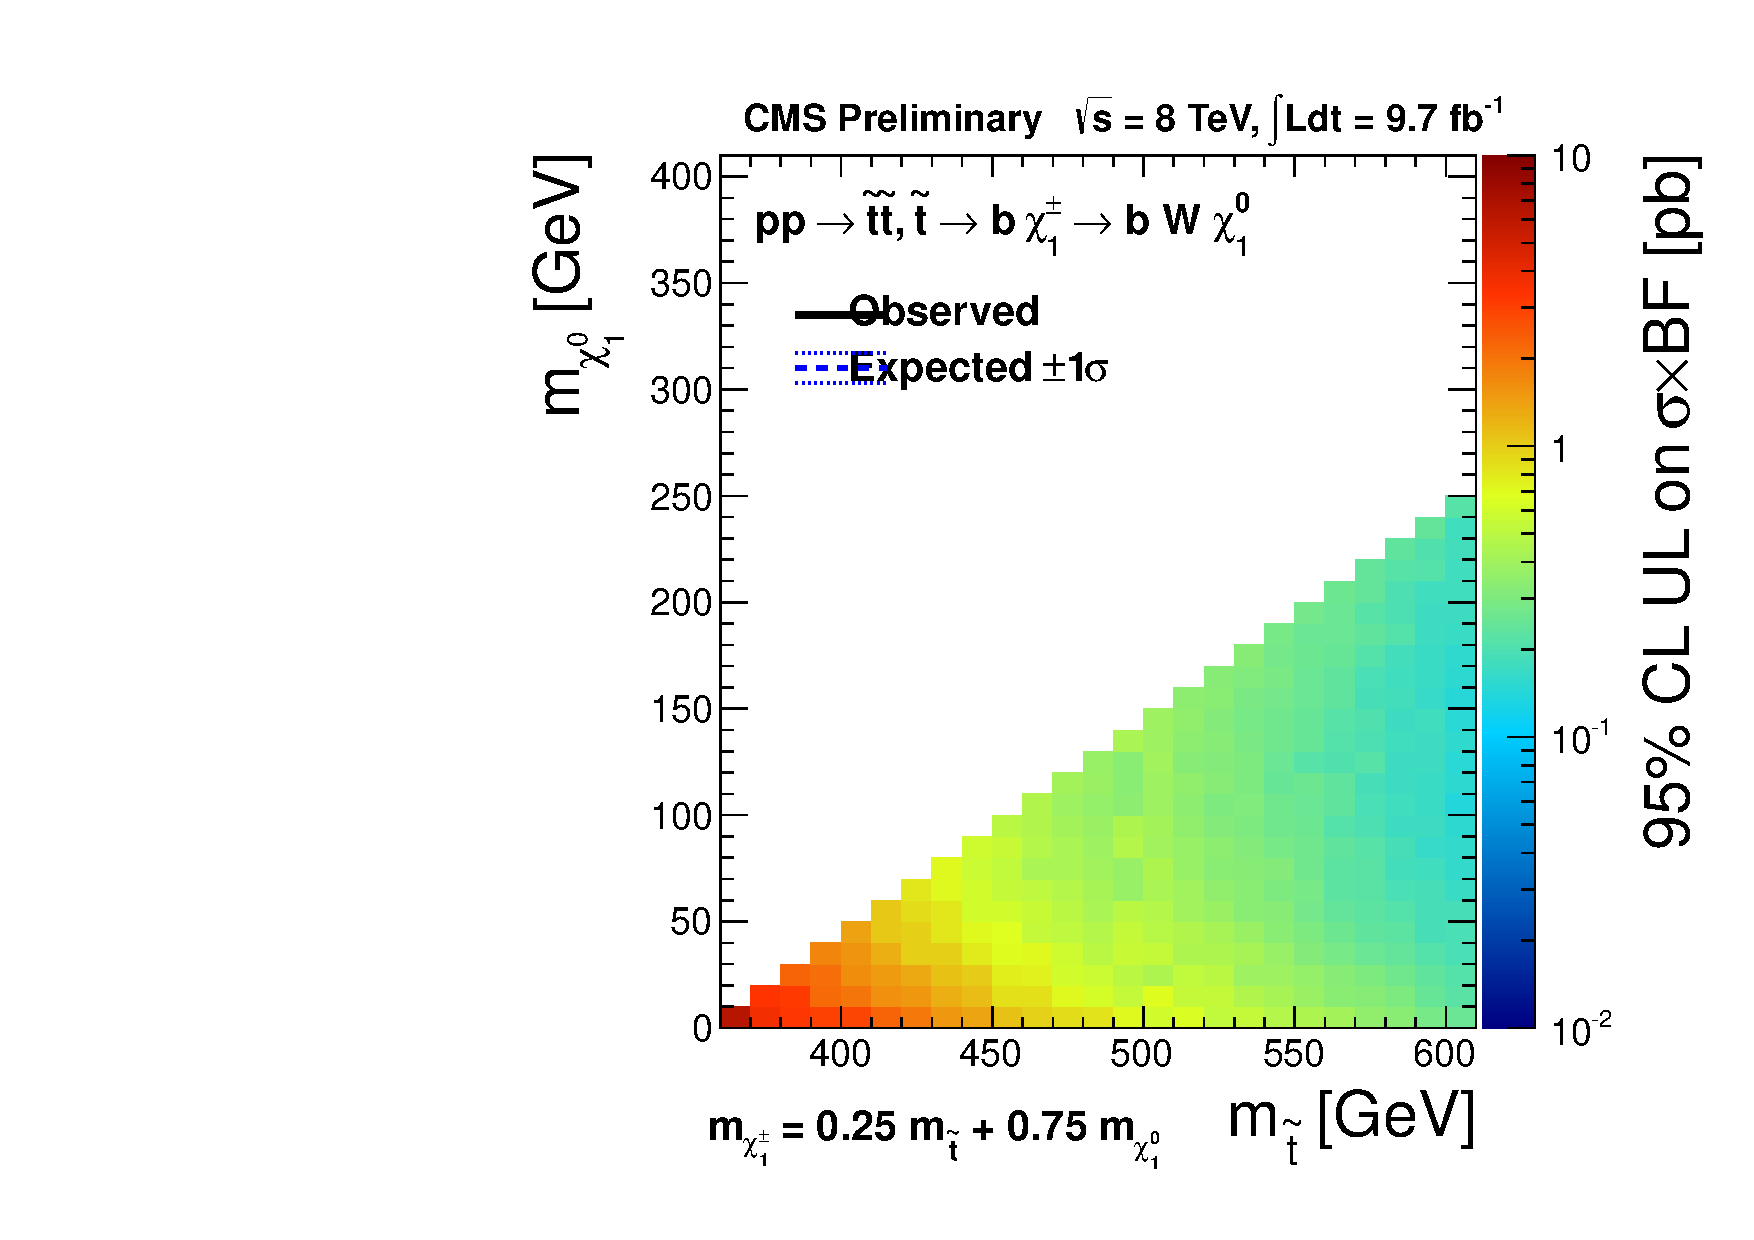
\includegraphics[height=6.5cm]{plots/combinePlots_T2bw_x25.pdf}%
       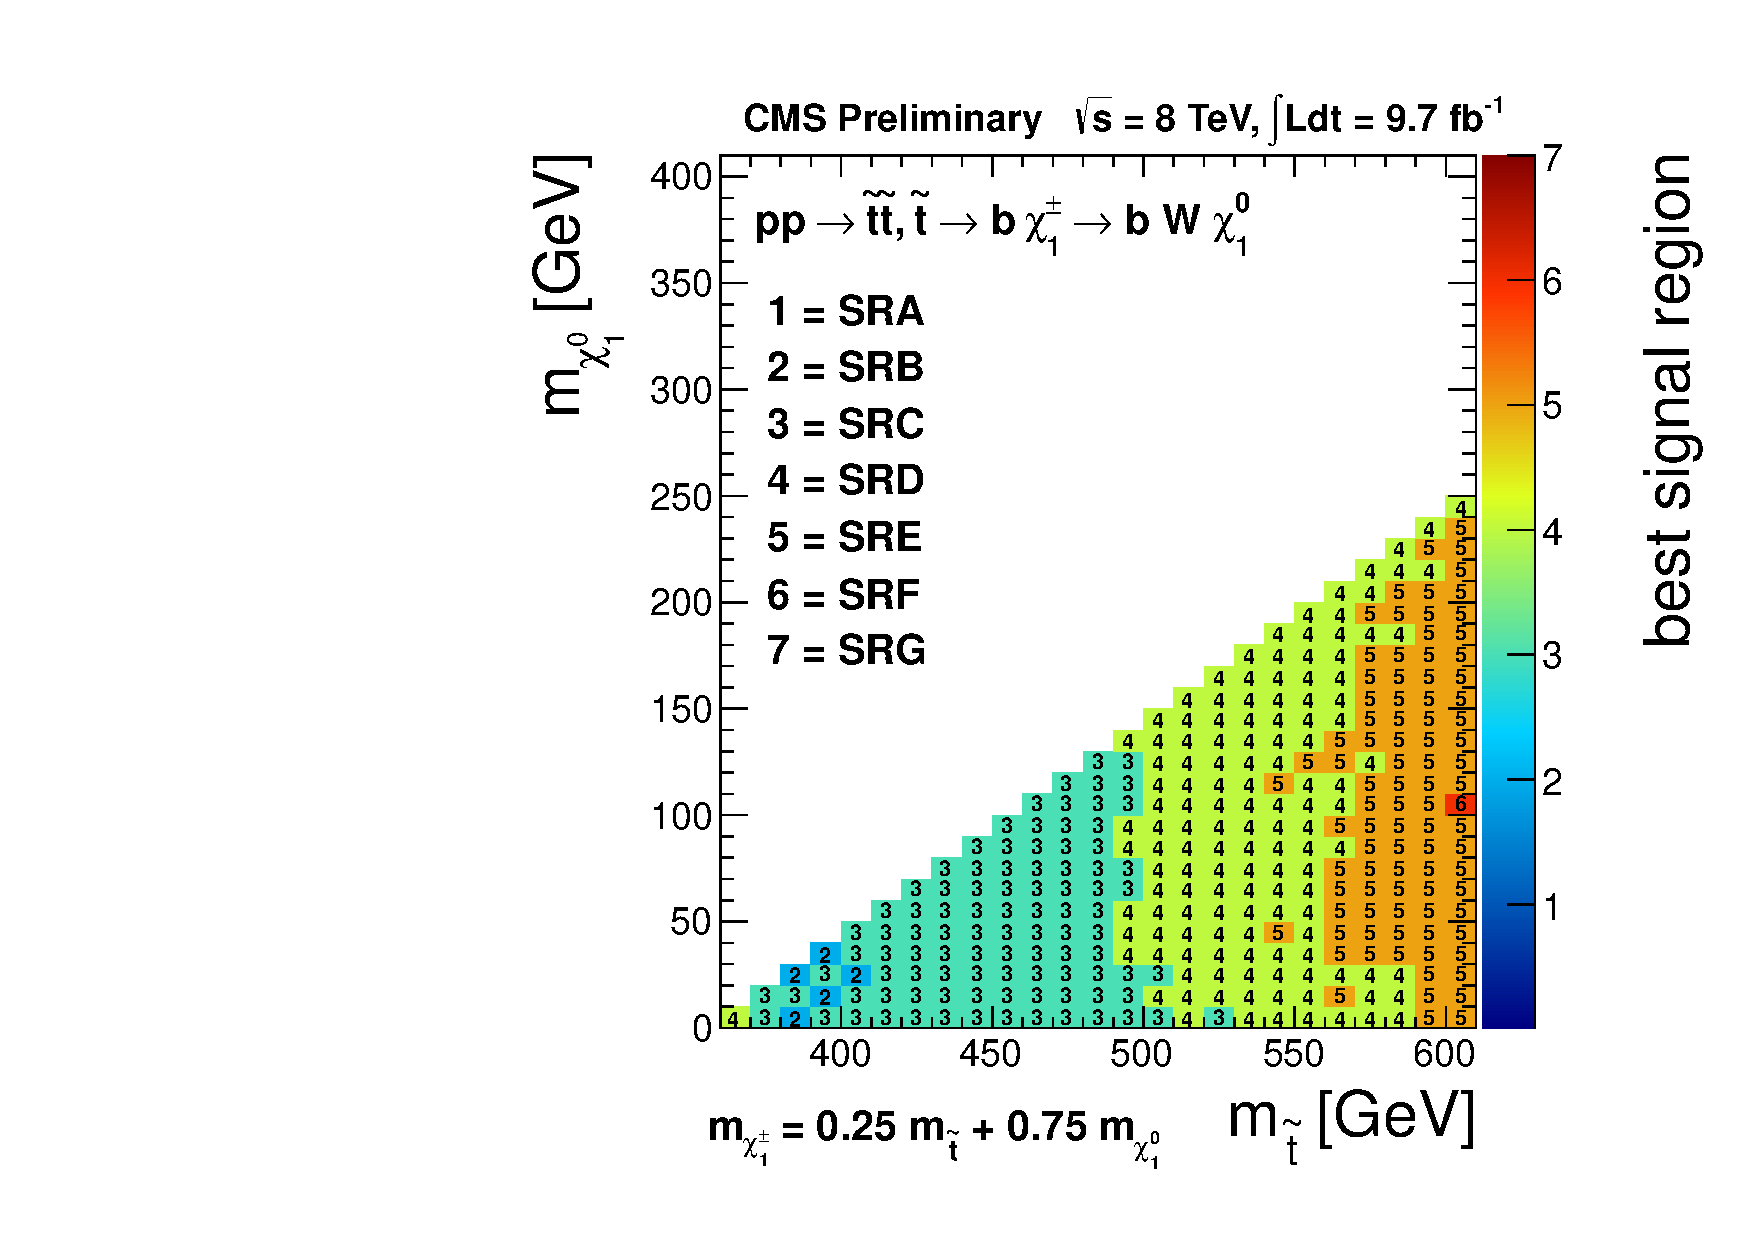
\includegraphics[height=6.5cm]{plots/combinePlots_T2bw_x25_bestSignalRegion.pdf}
    \caption{Upper limit on the cross section for the T2bw model for
      x=0.7 (top), x=0.5 (middle) and x=0.25 (bottom) in
      the plane of stop vs. LSP mass, showing
      both the expected (dashed) and observed (solid curve) exclusion
      contours (left). The observed
      limit is selected from the signal region with the best expected
      limit (shown on right). All uncertainties are included and the
      dotted contours around the dashed expected limit correspond to
      the $\pm 1\sigma$ result.}
\label{fig:comblimitT2bw}
      \end{center}
\end{figure}

\clearpage



\subsection{Model dependence of the signal acceptance}
\label{sec:modeldependence}

The signal acceptance for T2tt events has a significant dependence on the model parameters, particularly the mixing angle of left- and right-handed stops.
Depending on the choice of mixing angle, the top quarks produced in the decay can have a polarization anywhere between
$+p_{\chi_1^0}/E_{\chi_1^0}$ and $-p_{\chi_1^0}/E_{\chi_1^0}$~\cite{0811.1024}, which for a massless $\chi_1^0$ becomes $\pm 1$.
For right-handed top quarks, the charged lepton is emitted preferentially in the direction parallel to the top velocity, resulting in larger lepton \pt\ and \mt.

The default signal MC used in this analysis has unpolarized top quarks. We estimate the impact of the top polarization on our signal acceptance by reweighting
our signal MC events to match the expected distribution of the charged lepton decay angle ($\theta^{*}$) corresponding to the choice of top polarizations of $\pm 1$.
The default and reweighted $\cos\theta^{*}$ distributions are shown in Figure~\ref{fig:cosThetaStar}, for the signal sample with $M(\sctop)=450$~GeV and $M(\chi_1^0)=0$~GeV.
Note that this is only an approximate study, because the angular distribution is in fact triply differential. We attempt to account for the dominant effect.

\begin{figure}[hbt]
  \begin{center}
	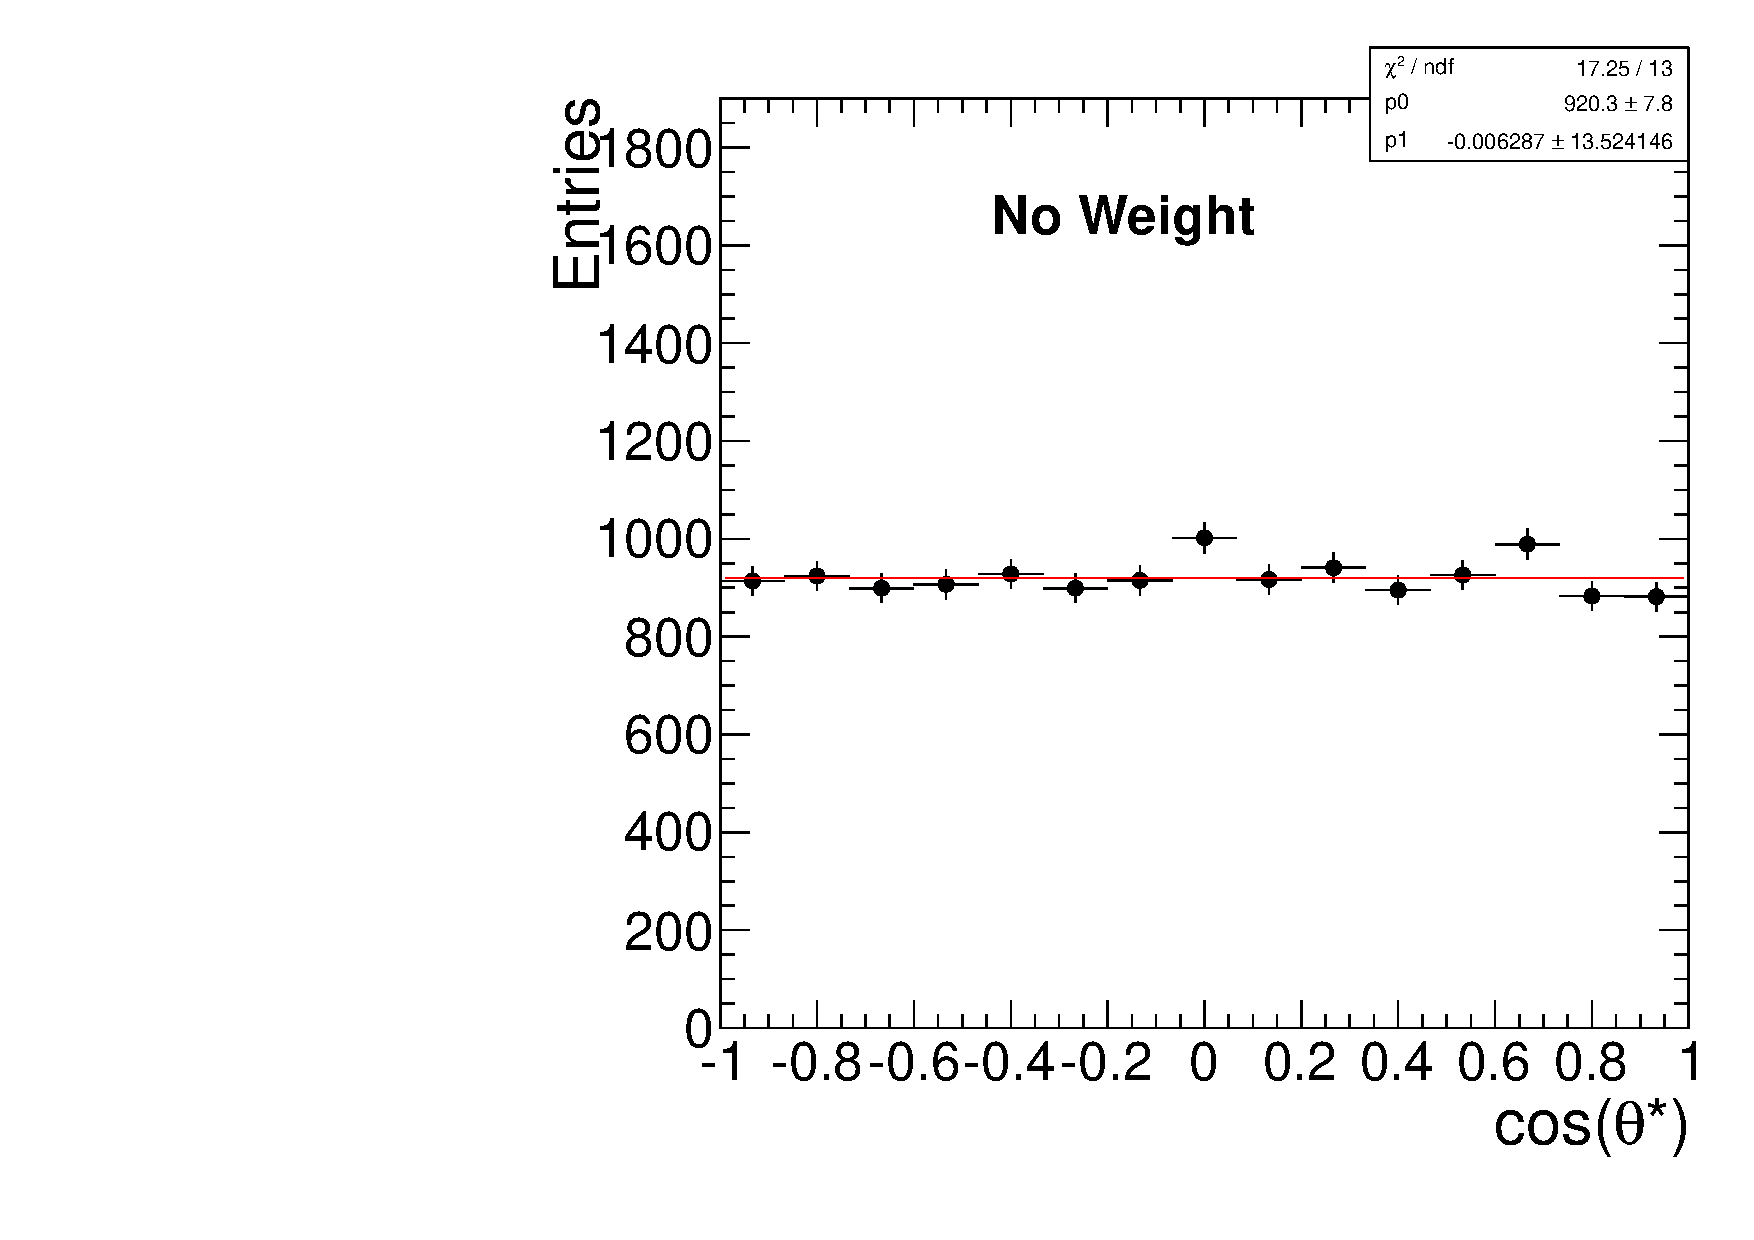
\includegraphics[width=0.325\linewidth]{plots/costheta.pdf}
	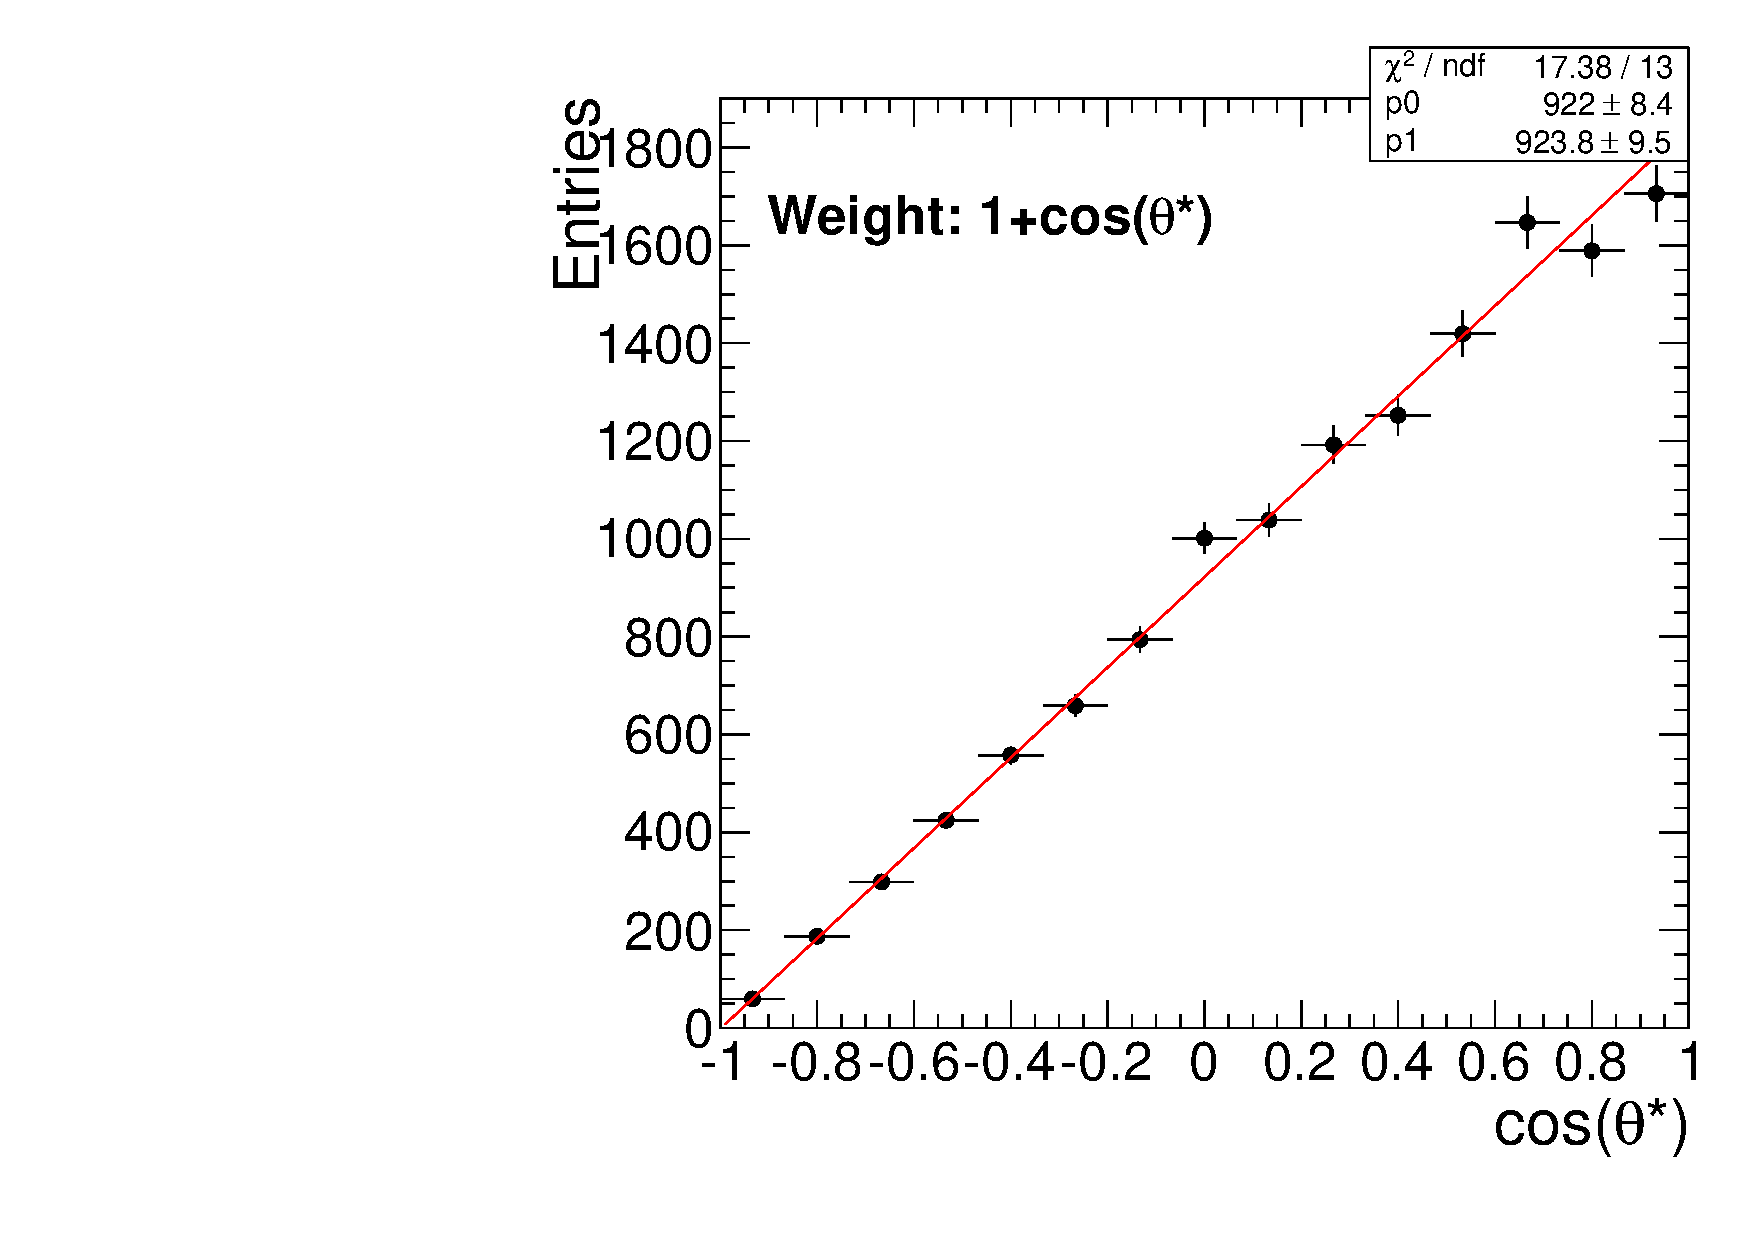
\includegraphics[width=0.325\linewidth]{plots/costheta_1p.pdf}
	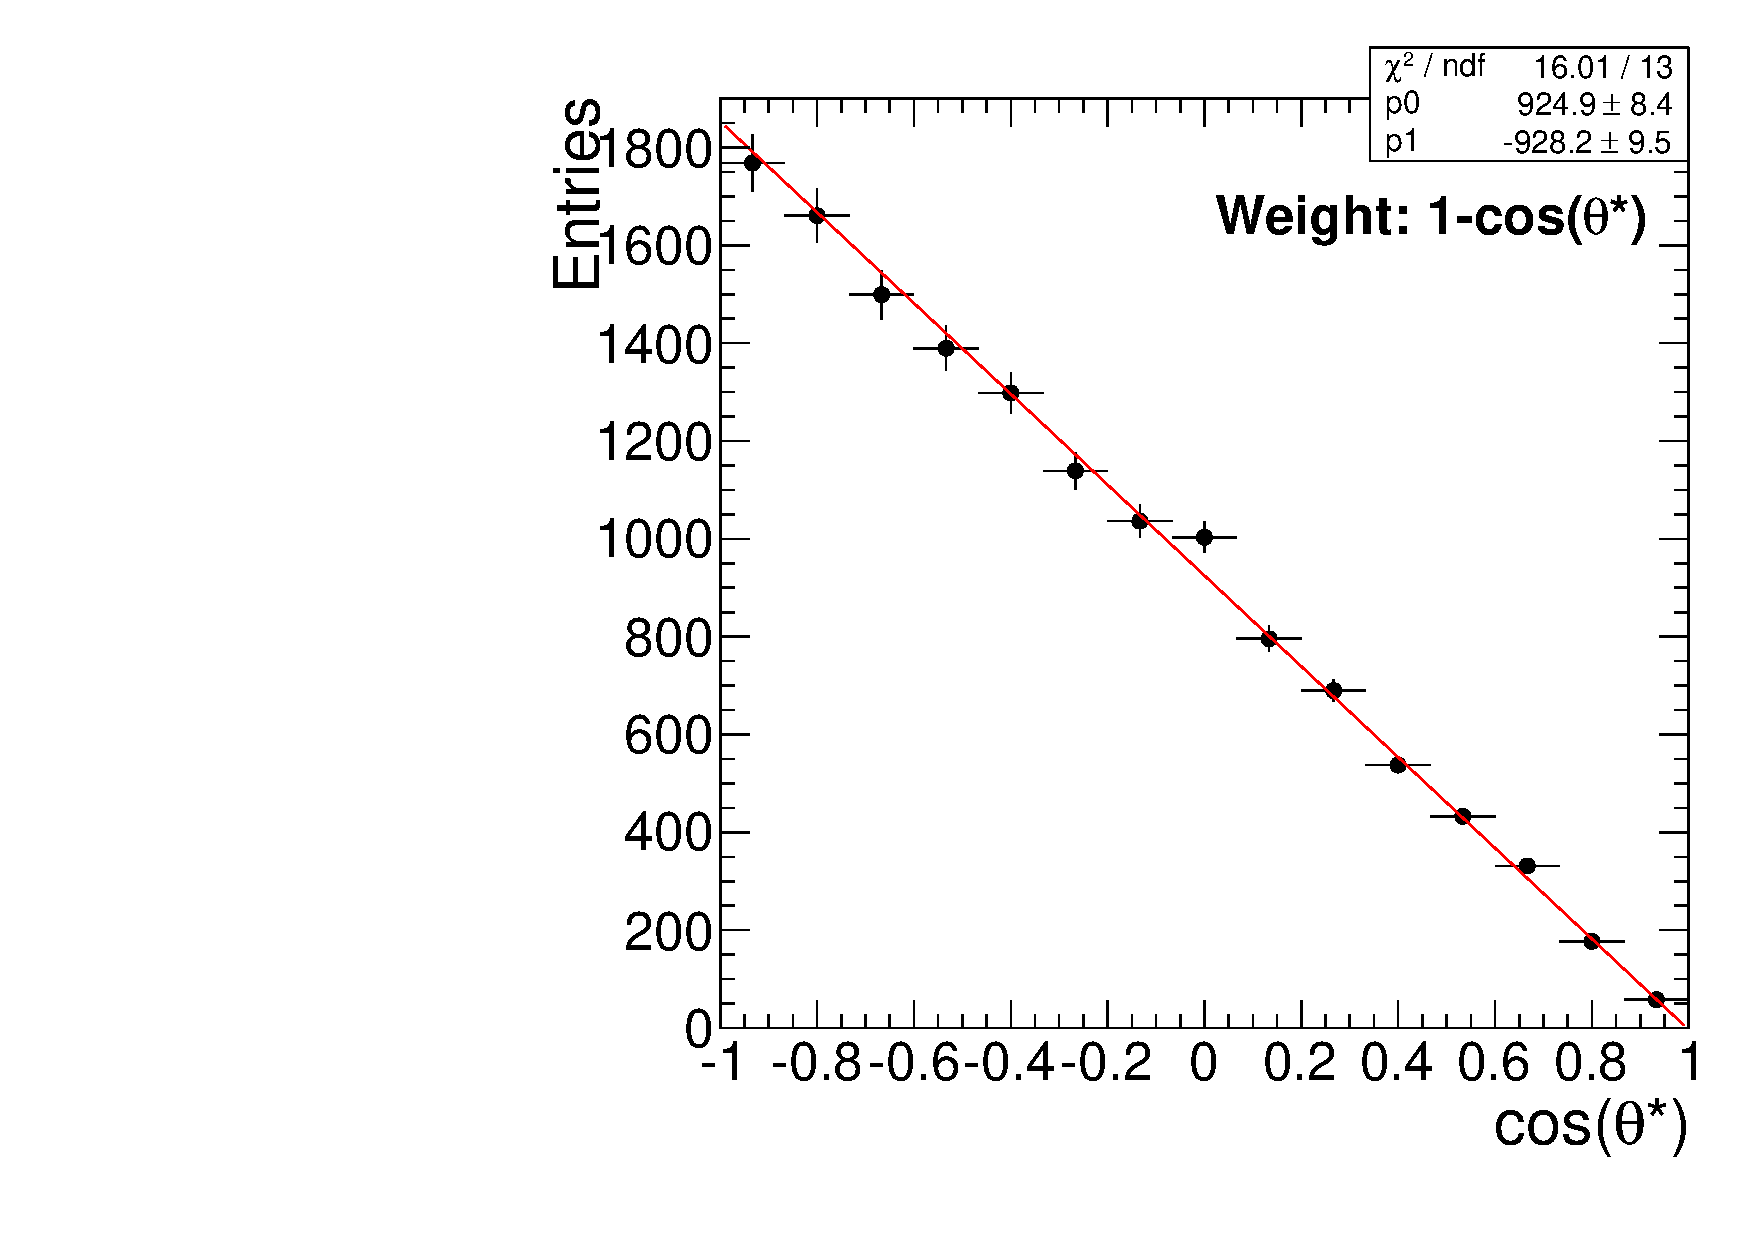
\includegraphics[width=0.325\linewidth]{plots/costheta_1m.pdf}
	\caption{
	  \label{fig:cosThetaStar}\protect 
          The default and reweighted $\cos\theta^{*}$ distributions for the signal sample with $M(\sctop)=450$~GeV and $M(\chi_1^0)=0$~GeV. The $1 \pm \cos\theta^{*}$ weightings correspond to top polarizations of $\pm 1$.}
  \end{center}
\end{figure}

We find that reweighting to simulate a top polarization of +1 increases the signal acceptance by 16-24\% relative to the default MC,
while simulating a top polarization of -1 decreases the signal acceptance by a similar amount. The results for the individual signal regions are given in Table~\ref{tab:AcceptanceChange}.

\begin{table}[!h]
\begin{center}
\begin{tabular}{l||c|c|c|c|c|c|c}
\hline
Sample              & SRA & SRB & SRC & SRD & SRE & SRF & SRG\\
\hline
\hline
$P=+1$ 	  & $+22\%$ & $+17\%$ & $+16\%$ & $+19\%$ & $+22\%$ & $+21\%$ & $+24\%$ \\
$P=-1$ 	  & $-22\%$ & $-17\%$ & $-16\%$ & $-19\%$ & $-22\%$ & $-21\%$ & $-24\%$ \\
\hline
\end{tabular}
\caption{  Change in signal acceptance after reweighing the events to simulate a top quark polarization ($P$) of $\pm 1$, for the signal sample with $M(\sctop)=450$~GeV and $M(\chi_1^0)=0$~GeV.
\label{tab:AcceptanceChange}}
\end{center}
\end{table}
